\documentclass[sigconf,review, anonymous]{acmart}
\usepackage{etex}
\usepackage{booktabs} % For formal tables
\usepackage[utf8]{inputenc}
\usepackage{xspace}
\usepackage{enumerate}
\usepackage{amsmath}
\usepackage{amsfonts}
\usepackage{amsthm}
\usepackage{amsopn}
\usepackage{vaucanson-g}
\usepackage{numprint}
%\usepackage[toc,page]{appendix}
\usepackage{booktabs} % Required for the top and bottom rules in the table
\usepackage{float} % Required for specifying the exact location of a figure or table 
\usepackage{enumitem}
\usepackage{placeins}
\usepackage{graphicx} % Required for including images
\usepackage{lipsum} % Used for inserting dummy 'Lorem ipsum' text into the template
%\usepackage{amssymb}
\usepackage{rotating}
\usepackage{tikz}
\usetikzlibrary{automata,positioning}
\usepackage{verbatim}
\usepackage{xypic}
\usepackage{wasysym}
\usepackage{amsmath,amsthm,mathtools,bussproofs,turnstile}
\usepackage{listings}
\usepackage{calc}
%\usepackage{changes}

\newlength\mylength
\setlength\mylength{(\widthof{long long long long long}-\widthof{short})/2}
\setlength\arraycolsep{2pt}
% Copyright
%\setcopyright{none}
%\setcopyright{acmcopyright}
%\setcopyright{acmlicensed}
%\setcopyright{rightsretained}
%\setcopyright{usgov}
%\setcopyright{usgovmixed}
%\setcopyright{cagov}
%\setcopyright{cagovmixed}
\usepackage{booktabs}
\usepackage{array}
\newcolumntype{L}[1]{>{\raggedright\let\newline\\\arraybackslash\hspace{0pt}}m{#1}}
\newcolumntype{C}[1]{>{\centering\let\newline\\\arraybackslash\hspace{0pt}}m{#1}}
\newcolumntype{R}[1]{>{\raggedleft\let\newline\\\arraybackslash\hspace{0pt}}m{#1}}
%\ifCLASSOPTIONcompsoc
%  % IEEE Computer Society needs nocompress option
%  % requires cite.sty v4.0 or later (November 2003)
%  \usepackage[nocompress]{cite}
%\else
%  % normal IEEE
%  \usepackage{cite}
%\fi

% DOI
%\acmDOI{10.475/123_4}

% ISBN
%\acmISBN{123-4567-24-567/08/06}

%Conference
%\acmConference[ESEC/FSE'17]{ESEC/FSE Conference}{September 2017}{Paderborn, Germany} 
%\acmYear{2017}
%\copyrightyear{2017}

%\acmPrice{15.00}
\acmYear{2018}
\acmConference[ESEC/FSE 2018]{The 26th ACM Joint European Software Engineering Conference and Symposium on the Foundations of Software Engineering}{4–9 November, 2018}{Lake Buena Vista, Florida, United States}



\begin{document}

% author names and affiliations
% use a multiple column layout for up to three different
% affiliations

\title{Behavior Minimization Feedback for Unrealizable Specifications }


\author{
%M. Cerrutti$^+$, V. Braberman$^+$, N. D'Ippolito$^+$, S. Uchitel$^+$$^\dagger$\\
%
%\IEEEauthorblockA{$^+$Departamento de Computaci\'{o}n, FCEN, Universidad de Buenos Aires, Argentina\\
%$^\dagger$Departament of Computing, Imperial College, London}
}
%\renewcommand{\shortauthors}{M. Cerrutti et. al.}

%Theorem Environments
\newtheorem{theorem}{Theorem}[section]
\newtheorem{lemma}[theorem]{Lemma}
\theoremstyle{definition}
\newtheorem{definition}{Definition}[section]
\newtheorem{corollary}[theorem]{Corollary}


%valuations
\newcommand{\valuations}{\ensuremath{\mathbb{V}}}
\newcommand{\propositions}{\ensuremath{\mathbb{P}}\xspace}
\newcommand{\proposition}{\ensuremath{p}\xspace}
%\newcommand{\acceptingState}{acc}
%\newcommand{\acceptingSymbol}{\alpha}
%\newcommand{\acceptingSymbols}{\beta}
\newcommand{\executionDef}{\ensuremath{\varepsilon=s_0, \actionLabel_0, s_1, \ldots}\xspace}
\newcommand{\execution}{\ensuremath{\varepsilon}\xspace}

%clts
\newcommand{\cltsDefIdx}[1]{\ensuremath{#1 = \lparen S_{#1},} \ensuremath{\Sigma_{#1}, \Delta_{#1},} \ensuremath{s_{0}^{#1}, \propositions_{#1}, \valuations_{#1}\rparen}\xspace}
\newcommand{\cltsDefShareSigmaIdx}[1]{\ensuremath{#1 = \lparen S_{#1},} \ensuremath{\Sigma, \Delta_{#1},} \ensuremath{s_{0}^{#1}, \propositions_{#1},} \ensuremath{\valuations_{#1}\rparen}\xspace}
\newcommand{\cltsDef}{\ensuremath{E = (S, \Sigma, \Delta, s_{0}, \propositions, \valuations)}\xspace}
\newcommand{\cltsEmbeddingDef}[1]{\ensuremath{clts(#1) = (S, \Sigma, \Delta, s_{0}, \valuations)}\xspace}
\newcommand{\automaton}[1]{\ensuremath{#1 = (S_{#1}, \Sigma_{#1}, \Delta_{#1}, s_{0}^{#1})}\xspace}
\newcommand{\labelSet}{\ensuremath{\mathcal{L}}\xspace}
\newcommand{\actionLabel}{\ensuremath{L}\xspace}
\newcommand{\action}{\ensuremath{l}\xspace}
\newcommand{\traces}{\ensuremath{\emph{Tr}}}

%composition
\newcommand{\cltsComposition}[3]{{\ensuremath{#1 \parallel_{#3} #2 = \lparen S,$ $\Sigma_{#1} \cup \Sigma_{#2},$ $\Delta,$ $(s_{0}^{#1},s_{0}^{#2}),$ $\propositions_{#1} \cup \propositions_{#2}$ $\valuations\rparen}}\xspace}
\newcommand{\ltsAdjustment}[2]{{\ensuremath{#1 \pm #2 = \lparen S_{#1}\times S_{#2},$ $\Sigma_{#1} \cup \Sigma_{#2},$ $\Delta,$ $(s_{0}^{#1},$ $s_{0}^{#2})\rparen}}\xspace}

%control problem
\newcommand{\controlSet}{\ensuremath{\mathcal{C}}}
\newcommand{\nonControlSet}{\ensuremath{\mathcal{U}}}
\newcommand{\controlProblemDef}{\ensuremath{\controlProblem =\langle E,$ $\controlSet,$ $\varphi \rangle}\xspace}
\newcommand{\controlProblem}{\ensuremath{\mathcal{I}}}

%GS
\newcommand{\gsV}{{\ensuremath{\mathcal{V}}}\xspace}
\newcommand{\gsX}{{\ensuremath{\mathcal{X}}}\xspace}
\newcommand{\gsY}{{\ensuremath{\mathcal{Y}}}\xspace}
\newcommand{\gsTheE}{\ensuremath{{\theta_e}}\xspace}
\newcommand{\gsTheS}{\ensuremath{{\theta_s}}\xspace}
\newcommand{\gsRhoE}{\ensuremath{{\rho_e}}\xspace}
\newcommand{\gsRhoS}{\ensuremath{{\rho_s}}\xspace}

%FDS
\newcommand{\enumSet}[1]{\#(#1)}
\newcommand{\enumSetDef}{$\#:\mathcal{P}(\mathcal{M})\mapsto [0\ldots2^{|\mathcal{M}|}-1]$\xspace}
\newcommand{\fdsDefIdx}[1]{$#1= \langle \gsV_{#1},$ $\theta_{#1},$ $\rho_{#1},$ $\mathcal{J}_{#1},$ $\mathcal{C}_{#1}\rangle$\xspace}
\newcommand{\fdsD}{\ensuremath{\mathcal{D}}\xspace}
\newcommand{\fdsDef}{$\fdsD = \langle \gsV_d,$ $\theta_d,$ $\rho_d,$ $\mathcal{J}_d,$ $\mathcal{C}_d\rangle$\xspace}
\newcommand{\fdsControlProblemDef}{\ensuremath{\fdsControlProblem =\langle \gsX,} \ensuremath{\gsY,$ $\varphi \rangle}\xspace}
\newcommand{\fdsControlProblem}{\ensuremath{\mathcal{K}}\xspace}
%realizability theorems
\newcommand{\varState}[1]{\ensuremath{\hat{s}_{#1}}\xspace}
\newcommand{\varLabel}[1]{\ensuremath{\hat{l}_{#1}}\xspace}
\newcommand{\varphiLTL}{\ensuremath{\varphi_{FDS}}\xspace}
\newcommand{\varphiLTLDef}{\ensuremath{\varphiLTL = (\theta_e \implies \theta_s) \wedge (\theta_e \implies \square((\boxdot \rho_e) \implies \rho_s)) \wedge (\theta_e \wedge \rho_e \implies val(\varphi))}\xspace}
\newcommand{\varphiCLTS}{\ensuremath{\varphi_{CLTS}}}
\newcommand{\varphiCLTSDef}{\ensuremath{\varphiCLTS = ()}\xspace}
\newcommand{\varphiLtlFormula}{\ensuremath{(\theta_e \implies \theta_s) \wedge (\theta_e \implies \square((\boxdot \rho_e) \implies \rho_s)) \wedge (\theta_e \wedge \rho_e \implies val(\varphi))}}
\newcommand{\fdsEmbeddingDef}{\ensuremath{ltl(\controlProblem) = \langle \gsX,$ $\gsY,$ $\varphiLTL \rangle}\xspace}
\newcommand{\fdsEmbedding}{\ensuremath{ltl(\controlProblem)}\xspace}
\newcommand{\cltsCPEmbeddingDef}{\ensuremath{clts(\fdsControlProblem) =\langle E,$ $\controlSet,$ $\varphiCLTS \rangle}\xspace}
\newcommand{\cltsCPEmbedding}{\ensuremath{clts(\fdsControlProblem)}\xspace}


%formulae
\newcommand{\true}{\emph{true} }
\newcommand{\false}{\emph{false} }
\newcommand{\assume}{\phi}
\newcommand{\guarantee}{\gamma}
\newcommand{\invariant}{\rho}
\newcommand{\fluentp}[1]{\dot{#1}}
\newcommand{\fluent}{\emph{fl}}
\newcommand{\set}[1]{\{#1\}}
\newcommand{\gr}{{GR(1)}\xspace}
\newcommand{\sgr}{{SGR(1)}\xspace}
\newcommand{\G}{{\bf G}}
\newcommand{\F}{{\bf F}}
\newcommand{\X}{{\bf X}}
\newcommand{\U}{{\bf U}}


\begin{abstract}
At their early stages system specifications are usually unrealizable, in
other words, there is no system that can be built to satisfy its goals under
the assumed environment conditions. The cause for unrealizability can be
boiled down to the fact that stated goals are too strong, the assumptions are
too weak, or (commonly) a subtle combination of both.  Providing engineers
feedback that allows to understand the cause for unrealizability is
necessary if specifications are to be evolved into realizable ones.

In this paper, we propose a technique that minimizes the behavior of an
unrealizable \gr specification while preserving non-realizability, thus allowing
engineers to focus on core behavior that causes unrealizability. The technique assumes an automata-based description of the environment 
%and 
%This is the first technique that is designed to be used to provide feedback for \gr synthesis problems in which the environment is described as an automaton and the goals as liveness LTL formulas. 
%differs from existing feedback techniques as it reduces (rather than augmenting) allowable behavior while preserving unrealizability. 
and returns a model that preserves the cause for unrealizability in the sense that the environment's strategy for beating the system in the minimized model is also a winning strategy in the original model. 

%The technique has also the potential to complement existing techniques that assume a specification only in LTL form and that work by syntactic, rather than semantic, minimization.
\end{abstract}

\maketitle
%\IEEEpeerreviewmaketitle
% We no longer use \terms command
%\terms{Theory}

%\keywords{Unrealizability, Debugging, Formal Specifications}




\section{Introduction}
%specifications are hard to write properly and stay unrealizable for a long time


Requirements are naturally split between goals the system-to-be is expected to achieve and
assumptions that the system-to-be can rely on to fulfill its goals ~\cite{Jackson:1995,Letier:2002}. The question to be asked then is one of realizability: Is it possible to build a system that can monitor its environment and react through its capabilities in order to guarantee its goals as long as the environment fulfils the assumptions?

At early stages specifications are usually unrealizable ~\cite{Letier:2002}. There can be multiple causes for unrealizability including lack of monitorability and controllability, and over-idealization of goals and assumptions. Goals in their first formulations tend to be stronger than what can be reasonably required and assumptions tend to be too weak, failing to rule out exceptional circumstances that the system cannot deal with ~\cite{vanLamsweerde:2000}. 

Unfortunately, the cause for unrealizability tends to be the result of a combination of issues and is not easy to detect or understand. Providing engineers feedback that allows them to understand the cause for unrealizability is highly desired if specifications are to be evolved into realizable ones that can then be implemented. 

In general the process of producing a running system from a specification is manual and laborious. However, in some settings this process can be done automatically, ensuring a correct by construction system. This is the case for systems studied by supervisory control ~\cite{ramadge:1989}, FOND planning ~\cite{daniele:2000} and controller synthesis ~\cite{Maoz:2014,Bloem:2012}. 
In these settings, given a specification, an algorithm produces a strategy (that can be encoded as an automaton) that by monitoring and acting over its environment can guarantee the goals as long as the environment satisfies the assumptions. 

Synthesis algorithms only produce a system strategy if the original specification is realizable. 
When the specification is unrealizable, the engineer is left with the onerous task of understanding why no such strategy exists and, only after that, with the task of changing the specification.
\emph{In this paper, we propose a novel technique that provides feedback on unrealizable specifications}. 

Techniques for providing feedback on unrealizability have been proposed in ~\cite{DBLP:conf/fmcad/KonighoferHB09, DBLP:journals/scp/Schuppan12,DBLP:conf/fmcad/AlurMT13},
these assume that the specification is given in an expressive subset of Linear Temporal Logic (LTL) formulae, called \gr, and return a minimal subset of these that is still unrealizable. In other words, and in the spirit of unsatisfiable cores~\cite{Torlak:2008}, the technique produces a minimal subset of the original formulae that is still unrealizable. The intention is to allow engineers to focus on a portion of the original specification to identify the causes for unrealizability. 

In this paper we propose an alternative and potentially complementary technique for providing feedback on unrealizability. The technique \textit{differs} from existing ones in two ways. First and foremost, the approach minimizes allowable behavior while preserving unrealizability. The result is a model that exhibits a minimal representation of the original behavior while preserving the unrealizability causes present in the initial specification. In contrast, in existing approaches the reduced number of formulae results in a model that allows more behavior than originally specified. The second difference is that the approach presented herein assumes an automata-based description of the environment rather than an LTL specification. Automata-based specifications of the environment (e.g., labeled transition systems~\cite{Keller:1976}, statecharts~\cite{Harel:1987}, and process algebra~\cite{Milner:1982,Hoare:1983}) are common approaches to environment description in software engineering literature. There are a variety of software engineering tasks that have been approached using synthesis and automata-based descriptions (e.g,~\cite{Letier:2013:RMS,DIppolito:2013,Pistore:2004:PMW}). %Heaven:2009:GDA

The technique we present minimizes behavior  while preserving unrealizability. \textit{What does this mean?} A specification determines a game in which one player, the environment, tries to satisfy the assumptions while preventing the other player, the system-to-be, from achieving its goals. If the specification is unrealizable, it means that the environment has a playing strategy that always beats its opponent. In other words, no matter what the system-to-be does, it cannot achieve its goals. We refer to a minimization that preserves unrealizability as a process that produces a new model that has less behavior and for which the winning strategy of the environment also works in the original specification. This allows engineers to focus on the behavior of the original specification that causes unrealizability. 

%The technique has also the potential to complement existing techniques that assume a specification only in LTL form and that work by performing a declarative, rather than a behavior-based, minimization.

The paper is structured as follows. We first provide a motivating example as an informal overview of the proposed technique, we then present some preliminary definitions, namely to define formally a control problem and the notion of realizability, and then go on to define minimization and non-realizability preservation. In Section~\ref{sect:solution} we present the minimization algorithm and then discuss our way of validating the technique. We finally proceed with a discussion on related work and conclusions.
\clearpage
\section{Motivation}\label{sec:motivation}

We introduce a simple example to illustrate what we consider to be the complementary nature 
of both the presented approach and that of ~\cite{DBLP:conf/hvc/KonighoferHB10}. Suppose that the engineer is working on a specification consisting of two environmental boolean variables $x_1$ and $x_2$ and one system variable $y$. Variable $x_2$ (initially false) is required to swap its value at each step of the execution, while $x_1$ remains free. The value of $y$ is set at the start and kept fixed throughout the execution.
It is assumed that $x_1$ will hold true infinitely often while $x_1 \wedge x_2 \wedge y$ is also required to be satisfied infinitely often. This is the set of LTL formulae of the specification, with $\theta$ being the initial condition, $\rho_e$ the environmental safety restriction, $\varphi_e$ the liveness assumption and $\varphi_s$ the liveness guarantee:
\begin{center}
	\begin{tabular}{ r c l }
		$\theta$& $=$ &$\neg x_1 \wedge \neg x_2$\\
		$\rho_e$& $=$ &$\square(x_2 \leftrightarrow \bigcirc(\neg x_2))$\\
		$\rho_s$& $=$ &$\square(y \leftrightarrow \bigcirc(y))$\\		
		$\varphi_e$& $=$ &$\square \Diamond x_1$\\
		$\varphi_s$& $=$ &$\square \Diamond (x_1 \wedge x_2 \wedge y)$\\
	\end{tabular}
\end{center}

The automaton induced from this set of formulae is depicted in Fig. ~\ref{fig:konig_original_plant_2_clts}. At this point, the specification is not realizable because the environment can set $x_1$ to true only when $x_2$ is down, thus honoring the environmental assumption while avoiding the system to reach the winning valuation $x_1 \wedge x_2 \wedge y$. The minimization presented in ~\cite{DBLP:conf/hvc/KonighoferHB10} removes $\rho_e$ since it is unnecessary for the environment to swap $x_2$ regularly in order to win the (non) realizability game. This approach can be characterized as a syntactic minimization, whose purpose is to help the engineer when viewing the specification (in particular the safety part describing the behavior of the plant) as a set of LTL formulae. This approach, nonetheless, yields the automaton depicted in Fig. ~\ref{fig:konig_original_plant_k_2} which is, in fact, more complex in terms of its explicit behavior. Our approach is designed to simplify the semantic view of the specification, producing the automaton depicted in Fig. ~\ref{fig:konig_original_plant_c_2}. 

The syntactic minimization should help the engineer to focus on a smaller set of formulae while diagnosing the non realizability cause (in this case the too weak assumption $\varphi_e$) by getting rid of the irrelevant element $\rho_e$. Our approach simplifies the specification semantically instead, reducing the relevant behavior and showing that it is possible for the environment to avoid state 2 by never allowing $x_1$ and $x_2$ to happen simultaneously, while at the same time not restricting the system below its original capabilities. Notice that if we were allowed to add the assumption that both environmental variables occur simultaneously infinitely often ($\rho'_s = \square \Diamond x_1 \wedge x_2$) the specification would be realizable and choosing to raise $y$ at the beginning would be sufficient in order to guarantee our goal, as shown in Fig. ~\ref{fig:konig_strategy_2}. After fixing $y$ to true the environment can move freely as long as it visits state 2 infinitely often. If the engineer has this behavior in mind as her design intent, it should be easy to see that in the semantic minimization the desired state is unreachable, hopefully guiding her to the strengthening of the assumption.  In Fig. ~\ref{fig:konig_composition_2} we show the synchronous composition of the aforementioned strategy with our minimization. Note that after letting the system raise $y$ state 1 is visited only once and then the execution keeps moving between states 2 and 3 in order to keep the value of $x_2$ oscillating.
%\begin{figure}[bt]
%	\centering
%	\SmallPicture
%	%\ShowFrame
%	\VCDraw{
%		\begin{VCPicture}{(-4,-2.5)(4,9.5)}
%			\SetEdgeLabelScale{1.4}
%			\StateVar[0:\overline{x_1 x_2} y]{(-3,6)}{0}
%			\StateVar[1:x_1 x_2 y]{(0,8)}{1}
%			\StateVar[2:x_1 \overline{x_2} y]{(3,6)}{2}
%			\StateVar[3:\overline{x_1} x_2 y]{(0,4)}{3} 
%			\StateVar[4:\overline{x_1 x_2 y}]{(-3,0)}{4}			
%			\StateVar[5:x_1 x_2 \overline{y}]{(0,2)}{5}
%			\StateVar[6:x_1 \overline{x_2 y}]{(3,0)}{6}
%			\StateVar[7:\overline{x_1} x_2 \overline{y}]{(0,-2)}{7}   			  
%			\Initial[w]{0}
%			\Initial[w]{4}	
%			\ArcR{0}{1}{}
%			\ArcR{1}{0}{}
%			\ArcR{1}{2}{}						
%			\ArcR{2}{1}{}
%			\ArcR{2}{3}{}        
%			\ArcR{3}{2}{}
%			\ArcR{3}{0}{}
%			\ArcR{0}{3}{}
%			\ArcR{4}{5}{}
%			\ArcR{5}{4}{}
%			\ArcR{5}{6}{}						
%			\ArcR{6}{5}{}
%			\ArcR{6}{7}{}        
%			\ArcR{7}{6}{}
%			\ArcR{7}{4}{}
%			\ArcR{4}{7}{}			
%		\end{VCPicture}
%	}
%	\caption{Original Plant}
%\label{fig:konig_original_plant_2}
%\MediumPicture
%\end{figure}
\begin{figure}[bt]
\centering
\SmallPicture
%\ShowFrame
	\VCDraw{
	\begin{VCPicture}{(-4,-2.5)(4,9.5)}
		\SetEdgeLabelScale{1.4}
		\State[0]{(-5,3)}{init}
		\State[1]{(-2.5,3)}{init_e}		
		\State[2]{(-1.5,6)}{0}
		\State[3]{(1.5,8)}{1}
		\State[4]{(4.5,6)}{2}
		\State[5]{(1.5,4)}{3} 
		\State[6]{(-1.5,0)}{4}			
		\State[7]{(1.5,2)}{5}
		\State[8]{(4.5,0)}{6}
		\State[9]{(1.5,-2)}{7} 			  
		\Initial[w]{init}
		\EdgeL{init}{init_e}{\overline{x_1 x_2}}
		\ArcL{init_e}{0}{y}
		\ArcR{init_e}{4}{\overline{y}}	
		\ArcR{0}{1}{}\LabelL[.5]{x_1 x_2}
		\LArcR[.6]{1}{0}{\overline{x_1 x_2}}
		\ArcR{1}{2}{}\LabelL[.5]{\overline{x_2}}
		\LArcR[.6]{2}{1}{x_2}
		\ArcR{2}{3}{}\LabelL[.5]{\overline{x_1}x_2}
		\LArcR[.6]{3}{2}{x_1\overline{x_2}}
		\ArcR{3}{0}{}\LabelL[.5]{\overline{x_2}}
		\LArcR[.6]{0}{3}{x_2}
		\ArcR{4}{5}{}\LabelL[.5]{x_1 x_2}
		\LArcR[.6]{5}{4}{\overline{x_1 x_2}}
		\ArcR{5}{6}{}\LabelL[.5]{\overline{x_2}}
		\LArcR[.6]{6}{5}{x_2}
		\ArcR{6}{7}{}\LabelL[.5]{\overline{x_1}x_2}
		\LArcR[.6]{7}{6}{x_1\overline{x_2}}
		\ArcR{7}{4}{}\LabelL[.5]{\overline{x_2}}
		\LArcR[.6]{4}{7}{x_2}	
	\end{VCPicture}
}
	\caption{Original Plant}
	\label{fig:konig_original_plant_2_clts}
	\MediumPicture
\end{figure}
\begin{figure}[bt]
	\centering
	\SmallPicture
	%\ShowFrame
	\VCDraw{
	\begin{VCPicture}{(-4,-3.8)(4,10.3)}
		\SetEdgeLabelScale{1.4}
		\State[0]{(-5,3)}{init}
		\State[1]{(-2.5,3)}{init_e}		
		\State[2]{(-1.5,6.8)}{0}
		\State[3]{(1.5,8.8)}{1}
		\State[4]{(4.5,6.8)}{2}
		\State[5]{(1.5,4.8)}{3} 
		\State[6]{(-1.5,-.8)}{4}			
		\State[7]{(1.5,1.2)}{5}
		\State[8]{(4.5,-.8)}{6}
		\State[9]{(1.5,-2.8)}{7} 			  
		\Initial[w]{init}
		\LoopW{0}{}
		\LoopN{1}{}
		\LoopE{2}{}
		\LoopS{3}{}				
		\LoopW{4}{}
		\LoopN{5}{}
		\LoopE{6}{}
		\LoopS{7}{}			
		\EdgeL{init}{init_e}{\overline{x_1 x_2}}
		\ArcL{init_e}{0}{y}
		\ArcR{init_e}{4}{\overline{y}}	
		\VArcR{arcangle=10,ncurv=.9}{0}{1}{}\LabelL[.5]{x_1 x_2}
		\VArcR{arcangle=-55,ncurv=.9}{1}{0}{\overline{x_1 x_2}}
		\VArcR{arcangle=10,ncurv=.9}{1}{2}{}\LabelL[.5]{\overline{x_2}}
		\VArcR{arcangle=-55,ncurv=.9}{2}{1}{x_2}
		\VArcR{arcangle=10,ncurv=.9}{2}{3}{}\LabelL[.5]{\overline{x_1}x_2}
		\VArcR{arcangle=-55,ncurv=.9}{3}{2}{x_1\overline{x_2}}
		\VArcR{arcangle=10,ncurv=.9}{3}{0}{}\LabelL[.5]{\overline{x_2}}
		\VArcR{arcangle=-55,ncurv=.9}{0}{3}{x_2}
		\VArcR{arcangle=10,ncurv=.9}{4}{5}{}\LabelL[.5]{x_1 x_2}
		\VArcR{arcangle=-55,ncurv=.9}{5}{4}{\overline{x_1 x_2}}
		\VArcR{arcangle=10,ncurv=.9}{5}{6}{}\LabelL[.5]{\overline{x_2}}
		\VArcR{arcangle=-55,ncurv=.9}{6}{5}{x_2}
		\VArcR{arcangle=10,ncurv=.9}{6}{7}{}\LabelL[.5]{\overline{x_1}x_2}
		\VArcR{arcangle=-55,ncurv=.9}{7}{6}{x_1\overline{x_2}}
		\VArcR{arcangle=10,ncurv=.9}{7}{4}{}\LabelL[.5]{\overline{x_2}}
		\VArcR{arcangle=-50,ncurv=.9}{4}{7}{x_2}	
		\VArcL[.7]{arcangle=15,ncurv=.4}{0}{2}{x_1}
		\VArcL[.7]{arcangle=15,ncurv=.4}{2}{0}{\overline{x_1}}
		\VArcL[.7]{arcangle=15,ncurv=.4}{1}{3}{x_1}
		\VArcL[.7]{arcangle=15,ncurv=.4}{3}{1}{\overline{x_1}}
		\VArcL[.7]{arcangle=15,ncurv=.4}{4}{6}{x_1}
		\VArcL[.7]{arcangle=15,ncurv=.4}{6}{4}{\overline{x_1}}
		\VArcL[.7]{arcangle=15,ncurv=.4}{5}{7}{x_1}
		\VArcL[.7]{arcangle=15,ncurv=.4}{7}{5}{\overline{x_1}}		
	\end{VCPicture}
}	
	\caption{Minimization according to Könighoefer}
	\label{fig:konig_original_plant_k_2}
	\MediumPicture
\end{figure}
\begin{figure}[bt]
	\centering
	\SmallPicture
	%\ShowFrame
	\VCDraw{
	\begin{VCPicture}{(-4,.5)(4,8.5)}
		\SetEdgeLabelScale{1.4}
		\State[0]{(-5,4)}{init}
		\State[1]{(-2.5,4)}{init_e}		
		\State[2]{(-1.5,6)}{0}
		\State[3]{(1.5,8)}{1}
		\State[4]{(4.5,6)}{2}
		\State[5]{(1.5,4)}{3} 
		\State[6]{(-1.5,2)}{4}			
		\State[7]{(1.5,1)}{5}
		\State[8]{(4.5,1)}{6}			  
		\Initial[w]{init}
		\EdgeL{init}{init_e}{\overline{x_1 x_2}}
		\ArcL{init_e}{0}{y}
		\ArcR{init_e}{4}{\overline{y}}	
		\ArcL{0}{1}{}\LabelL[.5]{x_1 x_2}
		\ArcL{1}{2}{}\LabelL[.5]{\overline{x_2}}
		\LArcR[.5]{2}{3}{\overline{x_1}x_2}
		\LArcR[.6]{3}{2}{x_1\overline{x_2}}
		\ArcR{4}{5}{}\LabelL[.5]{x_1 x_2}
		\LArcR[.6]{6}{5}{x_2}
		\LArcR[.6]{5}{6}{\overline{x_2}}
	\end{VCPicture}
}
	\caption{Behavior minimization}
	\label{fig:konig_original_plant_c_2}
	\MediumPicture
\end{figure}
\begin{figure}[bt]
	\centering
	\SmallPicture
	%\ShowFrame
	\VCDraw{
		\begin{VCPicture}{(-4,3.5)(4,9.5)}
			\SetEdgeLabelScale{1.4}
			\State[0]{(-5,6)}{init}
			\State[1]{(-3,6)}{init_e}		
			\State[2]{(-1,6)}{0}
			\State[3]{(2,8)}{1}
			\State[4]{(5,6)}{2}
			\State[5]{(2,4)}{3} 		  
			\Initial[w]{init}
			\EdgeL{init}{init_e}{\overline{x_1 x_2}}
			\EdgeL{init_e}{0}{y}
			\ArcR{0}{1}{}\LabelL[.5]{x_1 x_2}
			\LArcR[.6]{1}{0}{\overline{x_1 x_2}}
			\ArcR{1}{2}{}\LabelL[.5]{\overline{x_2}}
			\LArcR[.6]{2}{1}{x_2}
			\ArcR{2}{3}{}\LabelL[.5]{\overline{x_1}x_2}
			\LArcR[.6]{3}{2}{x_1\overline{x_2}}
			\ArcR{3}{0}{}\LabelL[.5]{\overline{x_2}}
			\LArcR[.6]{0}{3}{x_2}	
		\end{VCPicture}
	}
	\caption{Realizable version strategy}
	\label{fig:konig_strategy_2}
	\MediumPicture
\end{figure}
\begin{figure}[bt]
	\centering
	\SmallPicture
	%\ShowFrame
	\VCDraw{
	\begin{VCPicture}{(-4,3.5)(4,9.5)}
		\SetEdgeLabelScale{1.4}
		\State[0]{(-5,6)}{init}
		\State[1]{(-3,6)}{init_e}		
		\State[2]{(-1,6)}{0}
		\State[3]{(2,8)}{1}
		\State[4]{(5,6)}{2}
		\State[5]{(2,4)}{3} 		  
		\Initial[w]{init}
		\EdgeL{init}{init_e}{\overline{x_1 x_2}}
		\EdgeL{init_e}{0}{y}
		\ArcL{0}{1}{x_1 x_2}
		\ArcL{1}{2}{\overline{x_2}}
		\ArcR{2}{3}{}\LabelL[.5]{\overline{x_1}x_2}
		\LArcR[.6]{3}{2}{x_1\overline{x_2}}
	\end{VCPicture}
}
	\caption{Composition of the strategy with the minimization}
	\label{fig:konig_composition_2}
	\MediumPicture
\end{figure}
\clearpage


We introduce a simple example to illustrate what we consider to be the complementary nature 
of both the presented approach and that of ~\cite{DBLP:conf/hvc/KonighoferHB10}. Suppose that the engineer is working on a specification consisting of two environmental boolean variables $x_1$ and $x_2$ and one system variable $y$. $x_2$ (initially false) is required to swap its valuation at each step of the execution, while $x_1$ remains free. The value of $y$ is derived from the conjunction of the two environmental variables.
It is assumed that $x_1$ will be set to true infinitely often while $y$ is required to also be satisfied infinitely often. The set of LTL formulae corresponding to this specification is as follow: 
\begin{center}
	\begin{tabular}{ r c l }
	$\theta_e$& $=$ &$\neg x_1 \wedge \neg x_2$\\
	$\theta_s$& $=$ &$\neg y$\\
	$\rho_e$& $=$ &$\square(x_2 \leftrightarrow \bigcirc(\neg x_2))$\\
	$\rho_s$& $=$ &$\square((x_1 \wedge x_2) \leftrightarrow y)$\\
	$\varphi_e$& $=$ &$\square \Diamond x_1$\\
	$\varphi_s$& $=$ &$\square \Diamond y$\\
\end{tabular}
\end{center}

The automaton induced from this set of formulae is depicted in Fig. ~\ref{fig:konig_original_plant}. The specification is not realizable because the environment can set $x_1$ to true only when $x_2$ is down, thus honoring the environmental assumption. The minimization presented in ~\cite{DBLP:conf/hvc/KonighoferHB10} removes $\rho_e$ since it is unnecessary for the environment to swap $x_2$ regularly in order to win the (non) realizability game. This approach can be characterized as a syntactic minimization, whose purpose is to help the engineer when viewing the specification (in particular the safety part describing the behavior of the plant) as a set of LTL formulae. This approach, nonetheless, yields the automaton depicted in Fig. ~\ref{fig:konig_original_plant_k} which is, in fact, more complex behavior-wise. Our approach is designed to simplify the semantic view of the specification, producing the automaton depicted in Fig. ~\ref{fig:konig_original_plant_c}. 

The syntactic minimization should help the engineer to focus on a smaller set of formulae while diagnosing the non realizability cause (in this case the too weak assumption $\varphi_e$) by getting rid of the irrelevant element $\rho_e$. Our approach simplifes the specification semantically, reducing the relevant behavior and showing that it is possible for the environment to avoid state 2 by never allowing $x_1$ and $x_2$ to happen simultaneously. If we were allowed to add the assumption that both environmental variables occur infinitely often ($\rho'_s = \square \Diamond x_1 \wedge x_2$) the specification would be realizable and the plant as is would be a proper controller, since it allows the environment to move freely as long as it visits state 2 infinitely often. If the engineer has this behavior in mind as her design intent, it should be easy for her to see that in our minimization the desired state is unreachable, hopefully guiding her to the strengthening of the assumption.  
\newpage
\begin{figure}[bt]
\centering
\SmallPicture
%\ShowFrame
\VCDraw{
	\begin{VCPicture}{(-4,-2.5)(4,2.5)}
		\SetEdgeLabelScale{1.4}
		\StateVar[0:\overline{x_1 x_2 y}]{(-3,0)}{1}
		\StateVar[2:x_1 x_2 y]{(0,-2)}{2}
		\StateVar[1:\overline{x_1} x_2 \overline{y}]{(3,0)}{3}
		\StateVar[3:x_1 \overline{x_2 y}]{(0,2)}{6}        
		\Initial[w]{1}
		\ArcR{1}{2}{}
		\ArcR{2}{1}{}
		\ArcR{6}{1}{}        
		\ArcR{1}{6}{}
		\ArcR{2}{3}{}
		\ArcR{3}{2}{}
		\ArcR{3}{6}{}
		\ArcR{6}{3}{}
	\end{VCPicture}
}
\caption{Original Plant}
\label{fig:konig_original_plant}
\MediumPicture
\end{figure}
\begin{figure}[bt]
	\centering
	\SmallPicture
	%\ShowFrame
	\VCDraw{
		\begin{VCPicture}{(-4,-3)(4,3)}
			\SetEdgeLabelScale{1.4}
			\StateVar[0:\overline{x_1 x_2 y}]{(-3,0)}{1}
			\StateVar[2:x_1 x_2 y]{(0,-2)}{2}
			\StateVar[1:\overline{x_1} x_2 \overline{y}]{(3,0)}{3}
			\StateVar[3:x_1 \overline{x_2 y}]{(0,2)}{6}        
			\Initial[n]{1}
			\LoopW{1}{}
			\LoopN{6}{}
			\LoopE{3}{}
			\LoopS{2}{}
			\ArcR{1}{2}{}
			\EdgeL{2}{1}{}
			\ArcR{1}{3}{}
			\ArcR{3}{1}{}
			\ArcR{6}{1}{}        
			\EdgeL{1}{6}{}
			\ArcR{2}{3}{}
			\EdgeL{3}{2}{}
			\ArcR{2}{6}{}
			\ArcR{6}{2}{}
			\ArcR{3}{6}{}
			\EdgeL{6}{3}{}
		\end{VCPicture}
	}
	\caption{Minimization according to Könighoefer}
	\label{fig:konig_original_plant_k}
	\MediumPicture
\end{figure}
\begin{figure}[bt]
	\centering
	\SmallPicture
	%\ShowFrame
	\VCDraw{
		\begin{VCPicture}{(-4,-3)(4,3)}
			\SetEdgeLabelScale{1.4}
			\StateVar[0:\overline{x_1 x_2 y}]{(-3,0)}{1}
			\StateVar[2:x_1 x_2 y]{(0,-2)}{2}
			\StateVar[1:\overline{x_1} x_2 \overline{y}]{(3,0)}{3}
			\StateVar[3:x_1 \overline{x_2 y}]{(0,2)}{6}        
			\Initial[w]{1}       
			\EdgeL{1}{6}{}
			\ArcR{3}{6}{}
			\ArcR{6}{3}{}
		\end{VCPicture}
	}
	\caption{Behavior minimization}
	\label{fig:konig_original_plant_c}
	\MediumPicture
\end{figure}
\clearpage
We motivate and informally introduce relevant concepts by discussing a small example inspired by~\cite{DBLP:conf/vmcai/PitermanPS06}. Suppose an engineer is writing the specification for an industrial
controller that needs to coordinate communication between various devices consuming data from different sensors via a shared bus according to the scheduling policy defined by an arbiter. 
A device acting as a master will raise a bus access requirement ($req$) 
%on the related bus input line 
to communicate with a specific sensor acting as a slave. 
The arbiter can then either grant access to the device ($grant$) or give the bus
to another master ($\overline{grant}$). For the latter case, the device denied permission will have to wait for the slave currently using the bus to raise a
ready signal ($hready$) indicating that it has finished operation.  Only then
will the device issue another requirement.  If access is granted then the device
will wait either for a slave confirmation ($hready$) or a $timeout$ event.
After the slave has finished operation the device will start to process the
received information ($process$). Should the slave issue a timeout message, a reset will be triggered ($reset$) to try and restore normal operation.  
The initial environment specification $E$, including safety assumptions and safety goals, is presented in Figure~\ref{fig:req_grant}, where
solid lines indicate non controllable actions and dotted lines indicate
controlled actions.  Non controllable actions are those that the environment
can trigger while controlled actions are triggered by the system. 
\begin{figure}[bt]
\centering
\SmallPicture
%\ShowFrame
\VCDraw{
    \begin{VCPicture}{(-4,-1.5)(4,2.3)}
        \SetEdgeLabelScale{1.4}
        \State[1]{(-3,0)}{1}
        \State[2]{(0,0)}{2}
        \State[3]{(3,1)}{3}
        \State[4]{(-0.5,3)}{4}
        \State[6]{(0,1.5)}{6}        
        \State[5]{(3,-1)}{5}
		\Initial[w]{1}
        \ChgEdgeLineStyle{dashed} %\EdgeLineDouble
        %\ChgEdgeLineWidth{1.5}
        \EdgeL{1}{2}{req}
        \ArcR[.3]{6}{1}{reset}        
        \VArcR{arcangle=-30}{4}{1}{process}        
        %\RstEdgeLineWidth{1}
        \RstEdgeLineStyle %\EdgeLineSimple
        \EdgeL{2}{3}{grant}
        \EdgeL[.75]{2}{5}{\overline{grant}}
        %\VArcR{arcangle=-20}{3}{6}{timeout}
        \ArcR[.6]{3}{6}{timeout}
        \ArcL{5}{1}{hready}
        \VArcR{arcangle=-30}{3}{4}{hready}
    \end{VCPicture}
}
\caption{Bus Access example ($E$)}
\label{fig:req_grant}
%%\vspace*{-4mm}
\MediumPicture
\end{figure}
\begin{figure}[bt]
\centering
\SmallPicture
%\ShowFrame
\VCDraw{
    \begin{VCPicture}{(-4,-1.5)(4,2)}
        \SetEdgeLabelScale{1.4}
        \State[1]{(-3,0)}{1}
        \State[2]{(0,-1)}{2}
        \State[3]{(3,0)}{3}
        \State[6]{(0,1)}{6}        
		\Initial[w]{1}
        \ChgEdgeLineStyle{dashed} %\EdgeLineDouble
        %\ChgEdgeLineWidth{1.5}
        \ArcR{1}{2}{req}
        \ArcR{6}{1}{reset}        
        %\RstEdgeLineWidth{1}
        \RstEdgeLineStyle %\EdgeLineSimple
        \ArcR{2}{3}{grant}
        %\VArcR{arcangle=-20}{3}{6}{timeout}
        \ArcR{3}{6}{timeout}
    \end{VCPicture}
}
\caption{Minimized Bus Access ($E_1$)}
\label{fig:req_grant_sub_1}
%\vspace*{-4mm}
\MediumPicture
\end{figure}
\begin{figure}[bt]
\centering
\SmallPicture
%\ShowFrame
\VCDraw{
    \begin{VCPicture}{(-4,-1.5)(4,2)}
        \SetEdgeLabelScale{1.4}
        \State[1]{(-3,0)}{1}
        \State[2]{(0,0)}{2}
        \State[3]{(3,1)}{3}
        \State[6]{(0,1.5)}{6}        
        \State[5]{(3,-1)}{5}
		\Initial[w]{1}
        \ChgEdgeLineStyle{dashed} %\EdgeLineDouble
        %\ChgEdgeLineWidth{1.5}
        \EdgeL{1}{2}{req}
        \ArcR[.3]{6}{1}{reset}        
        %\RstEdgeLineWidth{1}
        \RstEdgeLineStyle %\EdgeLineSimple
        \EdgeL{2}{3}{grant}
        \EdgeL[.75]{2}{5}{\overline{grant}}
        %\VArcR{arcangle=-20}{3}{6}{timeout}
        \ArcR[.7]{3}{6}{timeout}
        \ArcL{5}{1}{hready}
    \end{VCPicture}
}
\caption{Minimized Bus Access ($E_2$)}
\label{fig:req_grant_sub_2}
%\vspace*{-4mm}
\MediumPicture
\end{figure}


The goal of continually processing data from the board is captured
by the LTL liveness formula $\square\Diamond process$.  The assumption
that access to the bus will always eventually be granted to the device
is captured by the liveness formula $\square\Diamond grant$.
 Note that without further assumptions the environment is able to
 systematically produce $timeout$ actions even after granting the device access
 to the bus.  These two choices, picking $grant$ at state 2 and then
 $timeout$ at state 3 conform a winning strategy for the environment. In other
 words, no matter what the system does, the environment, by making these two
 choices always prevents the system goals from being achieved.
 
The  specification $E_{1}$ in Figure~\ref{fig:req_grant_sub_1} is a subgraph of $E$, describing an environment with strictly less behavior than that of $E$. Furthermore, the winning environment strategy for specification $E_1$ is also a winning environment strategy in $E$. Indeed,  $E_1$ cannot be further reduced while satisfying this strategy preserving property. Thus, $E_1$ can be thought of as a slice of the original environment specification that has removed behavior that is irrelevant with respect to a cause for unrealizability.

Assume that after analyzing this first unrealizability cause another assumption is added, forcing the environment to produce
$hready$ infinitely often ($\square\Diamond hready$) hoping to reach state 4,
thus realizing the goal.  It turns out that even after adding this
new assumption the specification remains unrealizable:  The environment
can avoid state 4 if it keeps track of the most recently satisfied assumption.
It can first grant access to the device and then produce a $timeout$. 
This will be the first cycle of its strategy, then it will deny access
 ($\overline{grant}$) and start over again.  This alternating strategy will allow the environment
 to fulfill its assumptions (producing $grant$ in the first cycle
 and $hready$ in the second) while avoiding to produce the expected
 outcome.  The LTS in Figure
 ~\ref{fig:req_grant_sub_2} represents a minimal slice of the original specification $E$ that captures the winning strategy of the environment. 
 
 

 %  Note that we are
 %trying to progressively fix the specification with the information
 %provided by our behavior minimization feedback . $E_2$ is of complimentary value
 %with respect to the counter strategy since it presents a more compact 
 %representation of the conflict (avoiding memory induced unrolling)
 %that is also canonical (since it does not need to fix an order for the
 %satisfaction of the assumptions on behalf of the environment).
 
 \begin{comment}
  
Our technique is in fact quiet different, in terms of behavior, to what is
achieved by minimizing the set of LTL formulae in a declarative specification.
To exemplify the difference, and the complementation between the declarative
and the behavior minimization we introduce a synthetic case where an engineer
wants to specify a zero triggered latch mechanism. The initial specification
involves only two signals: $x$ representing a single boolean input and $y$ the only
boolean output.  The idea is that the output should be kept constantly up 
once a zero boolean value has been fed to the system.
Before this $y$ must remain low.  
The specification is written as the conjunction of four LTL 
formulae as presented in table \ref{table:d-ff-spec}. 
Following the definitions from \cite{DBLP:conf/vmcai/PitermanPS06} $\theta_s$ stands for
an initial system formula, $\rho_s$ for a safety system formula and 
$\varphi_s$ for a system liveness formula.
The \textit{Initial condition} formula 
fixes the initial value for the output signal,
\textit{Wait for negative trigger} keeps the value of $y$ down as long as the input
is up and the output value has not yet been raised, \textit{Latch} keeps the 
output up after the initial raise and the \texttt{GR(1)} \textit{Goal} is to 
always eventually produce an output ($\square\Diamond(y)$).  After running our automated
translation we produced the LTS representation of the \textit{Game Structure}
definition.  We get the behavior depicted in Figure \ref{fig:fig.neg-trigger-latch-behavior}.
The $\uparrow$ suffix after a signal name means the the value is being raised ($x\uparrow$),
$\downarrow$ consequently means that value is being lowered ($x\downarrow$).  A $tick$ event
is added to show when the values can be kept constant at the current time step.
\begin{center}
 %\vspace*{-4mm}
\begin{table}[h]
  \begin{tabular}{ l  c  l }
	Name & Type & Requirement \\
    \hline
    Initial condition & $\theta_s$ & $y = 0$\\
    Wait for negative trigger & $\rho_s$ &$\square((x \wedge \neg y) \rightarrow \Circle(\neg y) )$ \\
    Latch & $\rho_s$ &$\square (y \rightarrow \Circle(y))$ \\   
    Goal &  $\varphi_s$ & $\square\Diamond(y)$\\
  \end{tabular}
  \caption{Zero triggered latch specification}
  \label{table:d-ff-spec}
 \end{table}
 %\vspace*{-12mm}
\end{center}
We wrote this specification in \texttt{RATSY}, run the minimization presented in
\cite{DBLP:conf/hvc/KonighoferHB10} (where the \textit{Latch} requirement was
considered irrelevant and removed) and then translated the minimized specification
to produce the LTS depicted in Figure 
\ref{fig:fig.neg-trigger-latch-behavior-formula-minimization}.  Understanding the specification
in terms of the conjunction of formulas we can see that the $Latch$ requirement is irrelevant
to the unrealizability cause since even if we allow the system to lower $y$ after its initial
raise, no output would be produced if the input is kept up.  Removing a formula is, in fact,
relaxing the behavior, this is expressed in the double lined states and transitions 
present in Figure \ref{fig:fig.neg-trigger-latch-behavior-formula-minimization}.  
We can see that the transitions added express the new behavior where the system is allowed
to lower $y$ after being raised.  Let us note that removing a formula means relaxing, 
thus augmenting, the behavior of the system.
\begin{figure}[bt]
\centering
\SmallPicture
%\ShowFrame
\VCDraw{
    \begin{VCPicture}{(-4,-5)(4,4)}
        \SetEdgeLabelScale{1.4}
        \State[1]{(0,3)}{1}
        \State[2]{(-3,2)}{2}        
        \State[3]{(-3,0)}{3}
        \State[4]{(3,-2)}{4}        
        \State[5]{(-3,-2)}{5}                
        \State[6]{(-3,-4)}{6}                        
        \State[7]{(3,2)}{7}                                
        \State[8]{(3,0)}{8}                                        
		\Initial[n]{1}
		\EdgeL{1}{2}{$x$\downarrow}
		\EdgeR{1}{7}{$x$\uparrow}		
		\EdgeR{8}{3}{$x$\downarrow}								
		\LoopW{3}{$tick$}
		\LoopE{8}{$tick$}		
		\LoopW{6}{$tick$}		
		\EdgeR{3}{4}{$x$\uparrow}
		\ArcR{5}{6}{$x$\uparrow}
		\ArcR{6}{5}{$x$\downarrow}		
        \ChgEdgeLineStyle{dashed} 
		\EdgeR{4}{6}{$y$\uparrow}		
		\EdgeL{2}{3}{$y$\downarrow}				
		\EdgeL{7}{8}{$y$\downarrow}						
		\EdgeR{3}{5}{$y$\uparrow}
		\EdgeR{4}{8}{$tick$}		
    \end{VCPicture}
}
%\vspace*{-2mm}
\caption{Zero triggered latch behavior.}
\label{fig:fig.neg-trigger-latch-behavior}
%\vspace*{-8mm}
\MediumPicture
\end{figure}

\begin{figure}[bt]
\centering
\SmallPicture
%\ShowFrame
\VCDraw{
    \begin{VCPicture}{(-4,-6)(4,5)}
        \SetEdgeLabelScale{1.4}
        \State[1]{(0,3)}{1}
        \State[2]{(-3,2)}{2}        
        \State[3]{(-3,0)}{3}
        \State[4]{(1,-1)}{4}        
        \State[5]{(-3,-2)}{5}                
        \State[6]{(-3,-4)}{6}                        
        \State[7]{(3,2)}{7}                                
        \State[8]{(3,0)}{8}                                        
        \StateLineDouble
		\State[9]{(1,-2.5)}{9}                         
        \State[10]{(-1,-2.5)}{10}                             
		\Initial[n]{1}
		\EdgeL{1}{2}{$x$\downarrow}
		\EdgeR{1}{7}{$x$\uparrow}		
		\ArcR{8}{3}{$x$\downarrow}								
		\LoopW{3}{$tick$}
		\LoopE{8}{$tick$}		
		\EdgeL[.8]{3}{4}{$x$\uparrow}
		\ArcR{5}{6}{$x$\uparrow}
		\ArcR{6}{5}{$x$\downarrow}	
		\EdgeLineDouble		
		\LoopS{9}{$tick$}	
		\ArcR[.3]{6}{9}{$tick$}
		\EdgeR{9}{10}{$x$\downarrow}
		\EdgeLineSimple
        \ChgEdgeLineStyle{dashed} 
		\EdgeL{2}{3}{$y$\downarrow}				
		\EdgeL{7}{8}{$y$\downarrow}						
		\ArcR{3}{5}{$y$\uparrow}
		\EdgeL{4}{8}{$tick$}		
		\EdgeLineDouble
		\EdgeR{10}{5}{$tick$}		
		\ArcR[.2]{10}{3}{$y$\downarrow}						
		\ArcR{4}{9}{$y$\uparrow}		
		\ArcR{9}{8}{$y$\downarrow}		
		\ArcR{5}{3}{$y$\downarrow}
		\VArcR{arcangle=-60,ncurv=1}{6}{8}{$y$\downarrow}				
    \end{VCPicture}
}
%\vspace*{-8mm}
\caption{Zero trig. latch formula based minimization.}
\label{fig:fig.neg-trigger-latch-behavior-formula-minimization}
%\vspace*{-4mm}
\MediumPicture
\end{figure}
We are looking at the same problem expressed from two 
different directions, thus making impossible a direct comparison of
the techniques.  One of our claims is that our approach is in
fact complimentary to that of the declarative minimization.
Our minimization produces the LTS depicted in Figure 
\ref{fig:fig.neg-trigger-latch-behavior-minimization}, where it
shows that the environment can easily win by playing to keep
$x$ up.  
It is important to note that when minimizing the control problem we must
keep it unrealizable while allowing the environment to have
a winning strategy that works in both the minimized and the original
control problem.
\begin{figure}[bt]
\centering
\SmallPicture
%\ShowFrame
\VCDraw{
    \begin{VCPicture}{(-5,-2)(5,2)}
        \SetEdgeLabelScale{1.4}
        \State[1]{(-3,0)}{1}
        \State[2]{(0,0)}{2}        
        \State[3]{(3,0)}{3}
		\Initial[w]{1}
		\EdgeL{1}{2}{$x$\uparrow}
		\LoopE{3}{$tick$}		
        \ChgEdgeLineStyle{dashed} 
		\EdgeL{2}{3}{$y$\downarrow}				
    \end{VCPicture}
}
%\vspace*{-8mm}
\caption{Zero trig. latch behavior based minimization.}
\label{fig:fig.neg-trigger-latch-behavior-minimization}
%\vspace*{-4mm}
\MediumPicture
\end{figure}
In both the declarative and the behavior-based approaches the
idea is that we are aiding the engineer in understanding the
cause on unrealizability.  If we think in terms of specification repair,
in this particular case if she were to add
a new assumption (\textit{input will eventually fall}), either as
$\square\Diamond(\neg x)$ or $\Diamond(\neg x)$ the specification
will become realizable.
In the next sections we will show how to automatically build a minimal sub-LTS that preserves a winning strategy for the environment (which is a cause of unrealizability).
%\subsection{On The Declarative vs Operational Approach}
To the best of our knowledge,
 previous work on the minimization of unrealizable
specifications has been focused on reducing the set of requirements expressed as LTL formulas.  
This is the approach taken in \cite{DBLP:conf/hvc/KonighoferHB10} and the
initial inspiration for our work.  Könighoefer et al. built their framework
from what was presented in \cite{DBLP:conf/vmcai/CimattiRST08} and in
\cite{DBLP:conf/vmcai/2008} where they took the \textit{delta debugging}
algorithm as a cost-effective minimization technique.\\
Even though the kind of properties being satisfied is the same, we differ
not only in the formalism under use but also in the nature of our minimization,
since we are not reducing the set of formulas but the explicit behavior expressed
as an automaton.\\
To clarify the difference we apply an automated translation
scheme to transform our operational control problem  into
a declarative specification.
The later is written as the conjunction of four \texttt{LTL} \cite{pnueli1977temporal}
formulas as presented in Table \ref{table:planar-robot-declarative-spec}. 
We follow the definitions from \cite{DBLP:conf/vmcai/PitermanPS06}. Our goal is to get a game structure that properly emulates the semantics
of the source control problem.  The idea is that both structures should
satisfy equivalent sets of LTL formulas.\\
The translation can be explained as follows:
we encode the automaton state space through a set of boolean system variables
that will express the binary representation at each particular state.  The 
target specification will have a boolean variable (or signal) for each source
event.  Monitored events from the source specification will be 
represented through environment variables ($\mathcal{X}$) and
controlled events through system variables ($\mathcal{Y}$).  
Suppose that we have the following control problem $\mathcal{I}=\langle E, \mathcal{C}, \varphi \rangle$,
with plant $E$ described as the LTKS $E = (S, \Sigma,\Delta, v:S \rightarrow 2^{\mathcal{F}} ,s_0)$, $\mathcal{F}=\{f_1, f_2 \}$ and where
$a,b,c \in \Sigma$, $c \in \mathcal{C}$, $v(s_i)=\{ f_1 \}, v(s_j)=\{f_2\}$ and
$(s_i, a, s_j)$,
$(s_j, a, s_k)$,
$(s_j,b,s_l)$,
$(s_j, c, s_m) \in \Delta$.
Each transition from the source automaton is translated into three 
different formulas ($enable_{sys}$, $enable_{env}$, $update$), two standing for enabling requirements:\\
\textbf{[$enable_{sys}$]}One for the environment ($env.enable_{i,a} \in \rho_e$) as an implication from current state 
and currently selected action into a disjunction of mutually exclusive conjunction 
of monitored event related signals declaring the set of next-step enabled
environment actions. Suppose that $s, act_c \in \mathcal{Y}$
and $act_a, act_b \in \mathcal{X}$.
\[
\square(s = i \wedge act_a \rightarrow \Circle((\neg act_a \wedge act_b)\vee(act_a \wedge \neg act_b) \vee (\neg act_a \wedge \neg act_b)))\]
\textbf{[$enable_{env}$]} One for the system ($sys.enable_{i,a} \in \rho_s$) as an implication from current state
and currently selected action into another implication 
from the negation of all monitored events to the
disjunction of mutually exclusive conjunction of controlled
event related signals declaring the set of next-step enabled
system actions.
\[
\square(s = i \wedge act_a \rightarrow \Circle((\neg act_a \wedge \neg act_b)\rightarrow (act_c)))\]
\textbf{[$update$]} The third transition requirement ($s.update_{i,a} \in \rho_s$) is the one 
effectively updating the automaton state representation.
\[
\square(s = i \wedge act_a \rightarrow \Circle(s = j))\]
Initial conditions ($\theta_s, \theta_e$) are set according to the initial state 
$s_0$ in the automaton and initially enabled actions.
The LTKS valuations, that predicate over the set $\mathcal{F}$ of 
fluents, is translated in with the proper system safety requirement.\\
Following this translation and starting with
the control problem presented for the planar robot
we get an equivalent game structure shown (abbreviated
leaving only formulas relevant to state $4$) in 
Table \ref{table:planar-robot-declarative-spec}.
\begin{center}
\begin{table}[h]
  \begin{tabular}{ L{2cm} c L{5cm} }
  \toprule
	Name  && Requirement \\
    Init. env.  &($\theta_e$) & $(sensor.disabled \veebar sensor.enabled)$ $ \wedge \neg timeout \wedge \neg data.rcvd$\\    
    Init. sys. &($\theta_s$) & $s = 0 \wedge \neg update.direction \wedge$ $\neg get.SLAM.location \wedge \neg get.GPS.location$\\
    
    \ldots  && \ldots \\
    
    $_{4 \rightarrow 3}$ $timeout$ &($\rho_s$)
    &$\square((s=4 \wedge timeout)\rightarrow \Circle(s=3))$ \\
    
    $_{4 \rightarrow 5}$ $data.rcvd$ &($\rho_s$)
    &$\square((s=4 \wedge data.rcvd)\rightarrow \Circle(s=5))$ \\
    
    \ldots  && \ldots \\
    
    $_{4\rightarrow 5}$ $data.rcvd$ enable$_{sys}$ &($\rho_s$)
    &$\square((s=4 \wedge data.rcvd)\rightarrow \Circle(update.direction \wedge \neg get.SLAM.location \wedge \neg get.GPS.location))$ \\    
    
    $_{4\rightarrow 5}$ $data.rcvd$ enable$_{env}$ &($\rho_e$)
    &$\square((s=4 \wedge data.rcvd)\rightarrow \Circle(\neg timeout \wedge \neg sensor.enabled \wedge \neg sensor.disabled \wedge \neg data.rcvd))$ \\        
    
    \ldots  && \ldots \\
    Goal   &($\varphi_s$) & $\square\Diamond(update.direction)$\\
    \bottomrule
  \end{tabular}
  \caption{Planar Robot Equivalent Game Structure}
  \label{table:planar-robot-declarative-spec}
 \end{table}
\end{center}
The Könighoefer et al. technique removes system requirements
only.  After applying their minimization the 
$_{4 \rightarrow 5} data.rcvd$ and $_{4 \rightarrow 5}$ $data.rcvd$ enable$_{sys}$ requirements are removed,
since relaxing the system this way does not affect 
the environment winning strategy.  The syntactic 
simplification actually augments the system transition
relation $\rho_{s}$ for the case where
$s=4 \wedge data.rcvd$ holds, implicitly adding a
$data.rcvd$ transition to every other state.  This
is feasible since the environment will always pick
$timeout$ over $data.rcvd$ when reaching state $4$. 
Aforementioned requirements 
($_{4 \rightarrow 5} data.rcvd$ and $_{4 \rightarrow 5}
data.rcvd$ enable$_{sys}$) are irrelevant to the 
non realizability cause, but removing them 
bloats the specification in terms of explicit behavior
since it adds more transitions.  We want to
improve the understanding of the problem by way
of simplification, this adds another point in favor
o a novel minimization technique, designed specifically
for behavior based (or operational) specifications.
%To exemplify the difference, and the complementation between the model-based
and the behavior-based minimization we introduce a synthetic case where an engineer
wants to specify a zero triggered latch mechanism. The initial specification
involves only two signals: $x$ representing a single boolean input and $y$ the only
boolean output.  The idea is that the output should be kept constantly up 
once a zero boolean value has been fed to the system.
Before this $y$ must remain as a zero.  
The specification is written as the conjunction of four \texttt{LTL} \cite{pnueli1977temporal}
formulas as presented in table \ref{table:d-ff-spec}. 
Following the definitions from \cite{DBLP:conf/vmcai/PitermanPS06} $\theta_s$ stands for
an initial system formula, $\rho_s$ for a safety system formula and 
$\varphi_s$ for a system liveness formula.
The \textit{Initial condition} formula 
fixes the initial value for the output signal,
\textit{Wait for negative trigger} keeps the value of $y$ down as long as the input
is up and the output value has not yet been raised, \textit{Latch} keeps the 
output up after the initial raise and the \texttt{GR(1)} \textit{Goal} is to 
always eventually produce an output ($\square\Diamond(y)$).  After running our automated
translation we produced the \texttt{LTS} representation of the \textit{Game Structure}
definition.  We get the behavior depicted in Figure \ref{fig:fig.neg-trigger-latch-behavior},
where again solid lines indicate monitored events and dashed lines indicate controlled events.
The $\uparrow$ suffix after a signal name means the the value is being raised ($x\uparrow$),
$\downarrow$ consequently means that value is being lowered ($x\downarrow$).  A $tick$ event
is added to show when the values could be kept constant at the current time step.
\begin{center}
\begin{table}[h]
  \begin{tabular}{ l  c  l }
	Name & Type & Requirement \\
    \hline
    Initial condition & $\theta_s$ & $y = 0$\\
    Wait for negative trigger & $\rho_s$ &$\square((x \wedge \neg y) \rightarrow \Circle(\neg y) )$ \\
    Latch & $\rho_s$ &$\square (y \rightarrow \Circle(y))$ \\   
    Goal &  $\varphi_s$ & $\square\Diamond(y)$\\
  \end{tabular}
  \caption{Zero triggered latch specification}
  \label{table:d-ff-spec}
 \end{table}
\end{center}
We wrote this specification in \texttt{RATSY}, run the minimization presented in
\cite{DBLP:conf/hvc/KonighoferHB10} (where the \textit{Latch} requirement was
considered irrelevant and removed) and then translated the minimized specification
to produce the \texttt{LTS} depicted in Figure 
\ref{fig:fig.neg-trigger-latch-behavior-formula-minimization}.  Understanding the specification
in terms of the conjunction of formulas we can see that the $Latch$ requirement is irrelevant
to the unrealizability cause since even if we allow the plant to lower $y$ after its initial
raise, no output would be produced if the input is kept up.  Removing a formula is, in fact,
relaxing the behavior, this is expressed in the double lined states and transitions 
present in Figure \ref{fig:fig.neg-trigger-latch-behavior-formula-minimization}.  
We can see that the transitions added express the new behavior where the plant is allowed
to lower $y$ after being raised.  Let us note that removing a formula means relaxing, 
thus augmenting, the behavior of the plant.
\begin{figure}[bt]
\centering
\SmallPicture
%\ShowFrame
\VCDraw{
    \begin{VCPicture}{(-4,-5)(4,4)}
        \SetEdgeLabelScale{1.4}
        \State[1]{(0,3)}{1}
        \State[2]{(-3,2)}{2}        
        \State[3]{(-3,0)}{3}
        \State[4]{(3,-2)}{4}        
        \State[5]{(-3,-2)}{5}                
        \State[6]{(-3,-4)}{6}                        
        \State[7]{(3,2)}{7}                                
        \State[8]{(3,0)}{8}                                        
		\Initial[n]{1}
		\EdgeL{1}{2}{$x$\downarrow}
		\EdgeR{1}{7}{$x$\uparrow}		
		\EdgeR{8}{3}{$x$\downarrow}								
		\LoopW{3}{$tick$}
		\LoopE{8}{$tick$}		
		\LoopW{6}{$tick$}		
		\EdgeR{3}{4}{$x$\uparrow}
		\ArcR{5}{6}{$x$\uparrow}
		\ArcR{6}{5}{$x$\downarrow}		
        \ChgEdgeLineStyle{dashed} 
		\EdgeR{4}{6}{$y$\uparrow}		
		\EdgeL{2}{3}{$y$\downarrow}				
		\EdgeL{7}{8}{$y$\downarrow}						
		\EdgeR{3}{5}{$y$\uparrow}
		\EdgeR{4}{8}{$tick$}		
    \end{VCPicture}
}
\vspace*{-2mm}
\caption{Zero triggered latch behavior.}
\label{fig:fig.neg-trigger-latch-behavior}
\vspace*{-4mm}
\MediumPicture
\end{figure}

\begin{figure}[bt]
\centering
\SmallPicture
%\ShowFrame
\VCDraw{
    \begin{VCPicture}{(-4,-6)(4,5)}
        \SetEdgeLabelScale{1.4}
        \State[1]{(0,3)}{1}
        \State[2]{(-3,2)}{2}        
        \State[3]{(-3,0)}{3}
        \State[4]{(1,-1)}{4}        
        \State[5]{(-3,-2)}{5}                
        \State[6]{(-3,-4)}{6}                        
        \State[7]{(3,2)}{7}                                
        \State[8]{(3,0)}{8}                                        
        \StateLineDouble
		\State[9]{(1,-2.5)}{9}                         
        \State[10]{(-1,-2.5)}{10}                             
		\Initial[n]{1}
		\EdgeL{1}{2}{$x$\downarrow}
		\EdgeR{1}{7}{$x$\uparrow}		
		\ArcR{8}{3}{$x$\downarrow}								
		\LoopW{3}{$tick$}
		\LoopE{8}{$tick$}		
		\EdgeL[.8]{3}{4}{$x$\uparrow}
		\ArcR{5}{6}{$x$\uparrow}
		\ArcR{6}{5}{$x$\downarrow}	
		\EdgeLineDouble		
		\LoopS{9}{$tick$}	
		\ArcR[.3]{6}{9}{$tick$}
		\EdgeR{9}{10}{$x$\downarrow}
		\EdgeLineSimple
        \ChgEdgeLineStyle{dashed} 
		\EdgeL{2}{3}{$y$\downarrow}				
		\EdgeL{7}{8}{$y$\downarrow}						
		\ArcR{3}{5}{$y$\uparrow}
		\EdgeL{4}{8}{$tick$}		
		\EdgeLineDouble
		\EdgeR{10}{5}{$tick$}		
		\ArcR[.2]{10}{3}{$y$\downarrow}						
		\ArcR{4}{9}{$y$\uparrow}		
		\ArcR{9}{8}{$y$\downarrow}		
		\ArcR{5}{3}{$y$\downarrow}
		\VArcR{arcangle=-60,ncurv=1}{6}{8}{$y$\downarrow}				
    \end{VCPicture}
}
\vspace*{-2mm}
\caption{Zero trig. latch formula based minimization.}
\label{fig:fig.neg-trigger-latch-behavior-formula-minimization}
\vspace*{-4mm}
\MediumPicture
\end{figure}
This comparison may seem unfair, and to some extent it is, if one
forgets that we are looking at the same problem expressed in two
quite different ways.  One of our claims is that our approach is in
fact complimentary to that of the model-based minimization.
Our minimization produces the plant depicted in Figure 
\ref{fig:fig.neg-trigger-latch-behavior-minimization}, where it
shows that the environment can easily win by playing to keep
$x$ up.  
It is important to note that when minimizing the plant we must
keep it unrealizable while allowing the environment to have
a winning strategy that works in both the minimized and the original
plant.
\begin{figure}[bt]
\centering
\SmallPicture
%\ShowFrame
\VCDraw{
    \begin{VCPicture}{(-5,-2)(5,2)}
        \SetEdgeLabelScale{1.4}
        \State[1]{(-3,0)}{1}
        \State[2]{(0,0)}{2}        
        \State[3]{(3,0)}{3}
		\Initial[w]{1}
		\EdgeL{1}{2}{$x$\uparrow}
		\LoopE{3}{$tick$}		
        \ChgEdgeLineStyle{dashed} 
		\EdgeL{2}{3}{$y$\downarrow}				
    \end{VCPicture}
}
\vspace*{-2mm}
\caption{Zero trig. latch behavior based minimization.}
\label{fig:fig.neg-trigger-latch-behavior-minimization}
\vspace*{-4mm}
\MediumPicture
\end{figure}
In the model-based and the behavior-based approaches the
idea is that we are aiding the engineer in understanding the
cause on unrealizability.  If we think in terms of specification repair,
in this particular case if she were to add
a new assumption (\textit{input will eventually fall}), either as
$\square\Diamond(\neg x)$ or $\Diamond(\neg x)$ the specification
will become realizable.



\end{comment}
 
\section{Preliminaries}


We model safety assumptions on the environment and goals for the system as composition of Labelled Transition Systems (LTS). 
\begin{definition}
	\label{def:LTS} \emph{(Labelled Transition Systems)} 
	A \emph{Labelled Transition System} (LTS) is $E =  (S, \Sigma, \Delta, s_0)$, where $S$ is a finite set of states, $\Sigma \subseteq Act$ is its {\em communicating alphabet}, $\Delta \subseteq (S \times \Sigma \times S)$ is a transition relation, and $s_0 \in S$ is the initial state.  We denote $\Delta(s)=\set{\act~|~(s,\act,s') \in \Delta}$. 
	An LTS is deterministic if $(s,\act,s')$ and $(s,\act,s'')$ are in $\Delta$ implies $s'=s''$.
	An execution of $E$ is a word $\varepsilon=s_0, \act_0, s_1, \ldots$ where $(s_i, \act_i, s_{i+1}) \in \Delta$. 
	A word $\pi$ is a trace (induced by $\varepsilon$) of $E$ if its the result of removing every $s_i$ from an execution $\varepsilon$ of $E$. 
	We denote the set of infinite traces of $E$ by $\traces(E)$. 
\end{definition}


\begin{definition}\label{def:parallelComposition}\emph{(Parallel Composition)}
	Let $P=(S_P,\Sigma_P,\Delta_P,s_{0_P})$ y $Q=(S_Q,\Sigma_Q,\Delta_Q,s_{0_Q})$ be two LTSs, then 
	the parallel composition $P\|Q$ is defined as $P \| Q = (S_P \times S_Q, \Sigma_P \cup \Sigma_Q, \Delta_{P\|Q}, (s_{0_P}, s_{0_Q}))$
	where $\Delta_{P\|Q}$ is the smallest relation satisfying that for all $s, t \in S_P$, $s',t' \in S_Q$ and $\ell \in \Sigma_P \cup \Sigma_Q$:
	\small
	\begin{gather*}
	(s,\ell,t) \in \Delta_{P} \wedge a \not\in \Sigma_Q \Rightarrow ((s,s'),\ell,(t,s')) \in \Delta_{P\|Q}\\
	(s',\ell,t') \in \Delta_{Q} \wedge \ell \not\in \Sigma_P \Rightarrow ((s,s'),\ell,(s,t')) \in \Delta_{P\|Q}\\
	(s,\ell,t) \in \Delta_{P} \wedge (s',\ell,t') \in \Delta_{Q} \Rightarrow ((s,s'),\ell,(t,t')) \in \Delta_{P\|Q} 
	\end{gather*}
	\normalsize
\end{definition}

The distinction between what an LTS can control and what it can monitor is enforced through the notion of 
{\em legal environment} taken from~\cite{DIppolito:2013}, and inspired in that of Interface Automata ~\cite{DBLP:conf/sigsoft/AlfaroH01}.
Intuitively, a controller does not block the actions that it does not control, and dually, the environment does not restrict controllable actions. 

\begin{definition} \label{def:IALTS} \emph{(Legal LTS)}
	Given LTSs $C = (S_C, \Sigma_C$, $\Delta_C$, $s_{0_C})$ and $E = (S_E,\Sigma_E,\Delta_E,s_{0_E})$, where $\Sigma$ is partitioned into actions controlled and monitored (non controllable) by $C$ ($\Sigma=\mathcal{C} \; \cup \;\mathcal{U}$), we say that $C$ is a legal LTS for $E$ if for all $(s_E,s_C) \in E\|C$ it holds that
	$\Delta_{E}(s_E)\cap \mathcal{C} \supseteq \Delta_{C}(s_C)\cap \mathcal{C}$ and also that  $\Delta_{E}(s_E)\cap \mathcal{U} \subseteq \Delta_{C}(s_C)\cap \mathcal{U}$.
	
\end{definition}

%We use $\Delta(s)$ to denote the set $\{\ell~|~(s,\ell,s') \in 
%\Delta \}$ and $\Delta(s,\ell)=\set{s'~|~(s,\ell,s')\in\ \Delta_E}$.
%We say that an LTKS is deterministic if, whenever $(s,\ell,s')$ and 
%$(s,\ell,s'')$ are in $\Delta$, $s'=s''$. 
%We use $\initialState{E}$ and $\states{E}$ to refer to $S_0$ and $S$ respectively.
%For deterministic LTKS, we also use $E\executes(a)$ to denote the LTKS $(S, A, P, \Delta, v, s)$ if $(s_0, a, s) \in \Delta$, and $E$ otherwise.
%\end{definition}
%\begin{definition}\emph{(Traces)}
%A trace of $E$ is $\pi\!=\!s_0,\ell_0,s_1,\ell_1,\cdots$, where $s_0$ is an initial state of $E$ and, for every $i\geq 
%0$, we have $(s_i,\ell_i,s_{i+1})\in \Delta$.
% We denote as $\pi|_{\Sigma}$ the 
%sequence that is the result of removing from $\pi$ all actions not in
%$\Sigma$. 
%We denote the set of infinite traces of $E$ by $\traces(E)$. 
%We will assume systems yield infinite traces. 
%\end{definition}

%\begin{definition}\emph{(Traces)}


%We describe liveness goals and assumptions using fluent linear temporal \gr formulae. Linear
%temporal logics (LTL) are widely used to describe behaviour requirements~\cite{CITA INCORRECTA: DBLP:conf/sigsoft/GiannakopoulouM03}.
%The motivation for
We use linear temporal logics on fluents (FLTL) since they provide a uniform framework
for specifying state-based temporal properties in event-based models~\cite{DBLP:conf/sigsoft/GiannakopoulouM03}. 
A \emph{fluent} \fluent is defined by a pair of sets and a Boolean value: $\emph{\fluent} = \langle I_{\emph{\fluent}}, T_{\emph{\fluent}}, \emph{Init}_{\emph{\fluent}} \rangle$, where $I_{\emph{\fluent}}\subseteq Act$ is the set of initiating actions, $T_{\emph{\fluent}}\subseteq Act$ is the set of terminating actions and $I_{\emph{\fluent}}\cap T_{\emph{\fluent}}=\emptyset$. 
A fluent may be initially \true or \false as indicated by \emph{Init}$_{\emph{\fluent}}$. 
Every action $\ell\in Act$ induces a fluent, namely $\fluentp{\ell}=\langle \ell, Act\setminus \set{\ell}, \false\rangle$. 
Finally, the alphabet of a fluent is the union of its terminating and initiating actions.

Let $\mathcal{F}$ be the set of all possible fluents over $Act$. 
An FLTL formula is defined inductively using the standard Boolean connectives and temporal operators $\bigcirc$~(next), $U$ (strong until) as follows: 
$\varphi ::= \fluent \mid \neg \varphi \mid \varphi \vee \psi \mid \X \varphi \mid \varphi U \psi,$
where $\fluent\in\mathcal{F}$. 
As usual we introduce $\wedge$, $\Diamond$ (eventually), and $\square$ (always) as syntactic sugar. 
Let $\Pi$ be the set of infinite traces over \emph{Act}.
The trace $\pi=\ell_0,\ell_1,\ldots$ satisfies a fluent $\emph{Fl}$ at position $i$, denoted $\pi,i \models \emph{Fl}$, if and only if at least one of the following conditions holds:
%\begin{list}{-} %{\leftmargin=3em}
\begin{itemize}
	\item $\emph{Init}_{\emph{Fl}} \wedge (\forall j \in \mathbb{N} \cdot 0 \leq j \leq i \rightarrow \ell_j \notin T_{\fluent})$
	\item $\exists j \in \mathbb{N} \cdot (j \leq i \wedge \ell_j \in I_{\fluent}) \wedge (\forall k \in \mathbb{N} \cdot j < k \leq i \ \rightarrow \ell_k \notin T_{\fluent})$
	%\end{list}
\end{itemize}

We will assume that FLTL formulae are equipped with the corresponding
fluent definition triples.
Formula satisfaction for FLTL is defined as follows: 
given an infinite trace $\pi$, the satisfaction of a formula $\varphi$ at position $i$, denoted $\pi,i\models\varphi$, is defined as shown in Figure~\ref{fig:back:satisfactionop}.  
\begin{figure}[bt]
	$$\begin{array}{lcl}
	\pi,i \models \fluent &\triangleq & \pi,i \models \fluent  \\
	\pi,i \models \neg \varphi & \triangleq & \neg(\pi,i \models \varphi) \\
	\pi,i \models \varphi \vee \psi &\triangleq& (\pi,i\models \varphi) \vee (\pi,i models \psi) \\
	\pi,i \models \bigcirc \varphi &\triangleq & \pi,1 \models \varphi \\
	\pi,i \models \varphi \bf U \psi &\triangleq&\exists j \geq i \cdot \pi,j \models \psi \wedge \forall \mbox{ }i \leq k < j \cdot \pi,k \models \varphi\\
	\end{array}$$
	\caption{Semantics for the satisfaction operator}
	\label{fig:back:satisfactionop}
	\vspace{-1em}
\end{figure}


We say that $\varphi$ holds in $\pi$, denoted $\pi\models\varphi$, if $\pi,0\models\varphi$. 
A formula $\varphi \in \mbox{FLTL}$ holds in an LTS $E$ (denoted $E \models \varphi$) if it holds on every infinite trace produced by $E$.

In this paper we restrict attention to \gr~\cite{DBLP:journals/jcss/BloemJPPS12} formulas as there are effective synthesis algorithms for this sub-logic~\cite{DBLP:journals/jcss/BloemJPPS12}. \gr formulae are of the form $\varphi = \bigwedge_{i=1}^n \square\Diamond \assume_i \implies \bigwedge_{j=1}^m \square\Diamond \guarantee_j$, where $\{\assume_1 \ldots \assume_n\}$ and $\{\guarantee_1 \ldots \guarantee_m\}$ are propositional FLTL formulae.

%%%represent the set of
%%%assumptions that should
%%%always eventually be satisfied in order to 
%%%always eventually satisfy the set of goals
%%%$\{\guarantee_1 \ldots \guarantee_m\}$.
%%%\gr is an expressive subset that has gained increased interest recently due to the development of tractable synthesis algorithms for it~\cite{DBLP:journals/jcss/BloemJPPS12}.

%From the FLTL definition it follows that many results for LTL can be
%easily extended to FLTL.

We now provide a standard definition of parallel composition of LTSs to support compositional construction of environment models~\cite{DBLP:journals/cacm/Hoare78}.
% which is defined as an LTS that models the asynchronous execution of composed models, interleaving non-shared actions but forcing synchronisation on shared actions. 

%%%%\begin{definition}\label{def:legalEnvironment}\emph{(Legal Environment)}
%%%%Given $M = (S_M, \Sigma_M, \Delta_M, s_{M_0})$ and  $P = (S_P,\Sigma_P,\Delta_P,s_{P_0})$ LTSs, where $L_M=\Sigma_{M_c}\cup \Sigma_{M_u}$, $\Sigma_{M_c}\cap
%%%%\Sigma_{M_u}=\emptyset$, $\Sigma_P=\Sigma_{P_c}\cup \Sigma_{P_u}$ and $\Sigma_{P_c}\cap
%%%%\Sigma_{P_u}=\emptyset$. We say that $M$ is a legal environment for $P$
%%%%if the interface automaton $M'=\langle S_M, \set{s_{M_0}}, \Sigma_{M_u},
%%%%\Sigma_{M_c}, \emptyset, \Delta_M \rangle$ is a \emph{legal environment}
%%%%for the interface automaton $P'=\langle S_P, \set{s_{P_0}},$
%%%%$\Sigma_{P_u}, \Sigma_{P_c}, \emptyset, \Delta_P \rangle$.
%%%%\end{definition}

%\begin{definition}\label{def:legalEnvironment}\emph{(Legal Environment)}
%Given $M = (S_M, \Sigma_{M_c}\cup \Sigma_{M_u},$ $ \Delta_M, s_{M_0})$ and  $P = (S_P,\Sigma_{P_c}\cup \Sigma_{P_u},\Delta_P,s_{P_0})$ LTSs.
%%where $\Sigma_M=\Sigma_{M_c}\cup \Sigma_{M_u}$, $\Sigma_{M_c}\cap \Sigma_{M_u}=\emptyset$, $\Sigma_P=\Sigma_{P_c}\cup \Sigma_{P_u}$ and $\Sigma_{P_c}\cap \Sigma_{P_u}=\emptyset$. 
%We say that $M$ is a legal environment for $P$ if the composition of the interface automata $M'=(S_M, s_{M_0}, \Sigma_{M_u}, \Sigma_{M_c}, \emptyset, \Delta_M)$ and $P'=(S_P, s_{P_0}, \Sigma_{P_u},$ $ \Sigma_{P_c}, \emptyset, \Delta_P)$ has no illegal states~\cite{DBLP:conf/sigsoft/AlfaroH01}. 
%\end{definition}

%

The following definitions are based on those presented in~\cite{alfaro01}.

\begin{definition}\label{def:IA}\emph{(Interface Automata~\cite{alfaro01})}
An \emph{Interface Automata} (IA) is $P=\langle V, V^{init}, \mathcal{A}^I, \mathcal{A}^O, \mathcal{A}^H, \mathcal{T} \rangle$ where,
\begin{itemize}
  \item $V$ is a set of states
  \item $V^{init} \subseteq V$ is a set of initial states, with
      $|V^{init}| \leq 1$.
  \item $\mathcal{A}^I$, $\mathcal{A}^O$ and $\mathcal{A}^H$
      are mutually disjoint sets of input, output and internal
      actions. $\mathcal{A}=\mathcal{A}^I \cup \mathcal{A}^O
      \cup \mathcal{A}^H$ denotes the set of all actions.
  \item $\mathcal{T} \subseteq V \times \mathcal{A} \times V$
      is the set of transitions.
\end{itemize}
\end{definition}

If $a\in \mathcal{A}^I$ (resp. $a\in \mathcal{A}^O$, $a\in
\mathcal{A}^H$), then $(v, a, v')$ is called an input (resp.
output, internal) transition. $\mathcal{T}^I$ (resp.
$\mathcal{T}^O$, $\mathcal{T}^H$) denotes the set of input (resp.
output, internal) transitions. We say that an interface automaton
$P$ is \emph{closed} if it only has internal actions (i.e.
$\mathcal{A}^I = \mathcal{A}^O = \emptyset$); otherwise, we say
that $P$ is \emph{open}. An action $a$ is \emph{enabled} at a state
$v\in V$ if there exists a $v'\in V$ such that
$(v,a,v')\in\mathcal{T}$. The sets $\mathcal{A}^I(v)$,
$\mathcal{A}^O(v)$ and $\mathcal{A}^H(v)$ denote the set of input,
output and internal actions that are enabled from state $v$, and
$\mathcal{A}(v)=\mathcal{A}^I(v) \cup \mathcal{A}^O(v)\cup
\mathcal{A}^H(v)$ is the set of all enabled actions from state $v$.
As an example consider the drill modelled with the IA automata in
Figure~\ref{fig:drillIA}. Whenever the drill receives a product to
be processed ($put$) it signals an actuator to start processing the
product ($process$). Afterwards, the sensors signal if the product
has been successfully processed ($processOk$) or not
($processFail$). If the processing was successful, the drill
informs that the product is now ready ($ack$) and can be picked up
($get$); or report an error ($nack$) and waits for the product to
be discarded ($discard$) otherwise.


\begin{definition}\label{def:composable}\emph{(Composable)}
Two interface automata $P=\langle V_P, V_P^{init}, \mathcal{A}_P^I,
\mathcal{A}_P^O, $ $\mathcal{A}_P^H, \mathcal{T}_P \rangle$ and
$Q=\langle V_Q, V_Q^{init}, \mathcal{A}_Q^I, \mathcal{A}_Q^O,
\mathcal{A}_Q^H, \mathcal{T}_Q \rangle$ are \emph{composable} if
\begin{center}
\begin{displaymath}
    \begin{array}{cc}
     \mathcal{A}_P^H \cap \mathcal{A}_Q = \emptyset & \mathcal{A}_P^I \cap \mathcal{A}_Q^I = \emptyset \\
     \mathcal{A}_P^O \cap \mathcal{A}_Q^O = \emptyset & \mathcal{A}_Q^H \cap \mathcal{A}_P = \emptyset
    \end{array}
\end{displaymath}
\end{center}
Let $shared(P, Q)= \mathcal{A}_P \cap \mathcal{A}_Q$.
\end{definition}

The composition of IAs $P$ and $Q$ is defined in stages. First, the
product automaton $P\otimes Q$, which coincides with the
composition of I/O automata~\cite{Lynch:1987:HCP:41840.41852},
except that since $P$ and $Q$ are not necessarily input-enabled,
some transitions present in $P$ or $Q$ may not be present in the
product.

\begin{definition}\label{def:ia-product}\emph{(Product)}
Given $P=\langle V_P, V_P^{init}, \mathcal{A}_P^I, \mathcal{A}_P^O, \mathcal{A}_P^H, \mathcal{T}_P \rangle$ and $Q=\langle V_Q, V_Q^{init}, \mathcal{A}_Q^I, \mathcal{A}_Q^O, \mathcal{A}_Q^H, \mathcal{T}_Q \rangle$ composable interface automata, their product is the interface automaton $P\otimes Q=\langle V_{P\otimes Q}, V_{P\otimes Q}^{init}, \mathcal{A}_{P\otimes Q}^I, \mathcal{A}_{P\otimes Q}^O, \mathcal{A}_{P\otimes Q}^H, \mathcal{T}_{P\otimes Q} \rangle$, where:\\
\begin{eqnarray*}
  V_{P\otimes Q} &=& V_P \times V_Q \nonumber\\
  V_{P\otimes Q}^{init} &=& V_{P}^{init} \times V_{Q}^{init} \nonumber\\
  \mathcal{A}_{P\otimes Q}^I &=& (\mathcal{A}_{P}^I \cup \mathcal{A}_{Q}^I)\setminus shared(P,Q)\nonumber\\
  \mathcal{A}_{P\otimes Q}^O &=& (\mathcal{A}_{P}^O \cup \mathcal{A}_{Q}^O)\setminus shared(P,Q)\nonumber\\
  \mathcal{A}_{P\otimes Q}^H &=& (\mathcal{A}_{P}^H \cup \mathcal{A}_{Q}^H)\cup shared(P,Q)\nonumber
\end{eqnarray*}
The transition relation is defined as follows:
\begin{eqnarray*}
% \nonumber to remove numbering (before each equation)
  \mathcal{T}_{P\otimes Q} &=& \set{((u,v),a,(u,v')) | (v,a,v')\in\mathcal{T}_{P} \wedge a\notin shared(P,Q) \wedge u\in V_Q} \nonumber\\
      &\cup & \set{((u,v),a,(u',v)) | (u,a,u')\in\mathcal{T}_{Q} \wedge a\notin shared(P,Q) \wedge v\in V_P} \nonumber\\
      &\cup& \set{((u,v),a,(u',v')) | (v,a,v')\in\mathcal{T}_{P} \wedge (u,a,u')\in\mathcal{T}_{Q} \wedge a\in shared(P,Q)} \nonumber
\end{eqnarray*}
\end{definition}

Recall that interface automata do not require input-enabledness.
Therefore given the product $P\otimes Q$ of two interface automata
$P$ and $Q$, may have states in which one of them produces an
output action that is input action for the other but it is not
enabled in that state, hence it is not accepted. Such a state is
called an \emph{Illegal} state. $Illegal(P,Q)$ denotes the set of
illegal states in the product $P\otimes Q$. In
Figure~\ref{fig:armIA} we present a robotic arm that places
products in the drill ($put$), waits for the drill to finish
($ack$) and finally picks the resulting product up ($get$). The
robotic arm assumes that once products have been placed in the
drill, they will be successfully processed. Hence, it cannot handle
failures. The IA $\drill \otimes \arm$ is shown in
Figure~\ref{fig:IAproduct}. As in the case of LTS parallel
composition, each state in $\drill \otimes \arm$ consists of a
state of $\drill$ together with a state of $\arm$, and each
transition represents either a joint step on both $\drill$ and
$\arm$ processes or an individual step on one of them. Consider the
following scenario, the arm places a product in the drill ($put$),
the drill starts processing ($process$) and its sensors signal a
failure ($processFail$). This sequence lead us to state $5$ of
$\drill \otimes \arm$, which corresponds to state $5$ of $\drill$
and $1$ of $\arm$. In state $5$, the sensors are signalling the
drill that something went wrong while processing the current
product, but the $\arm$ is not prepared to handle such situation.
Such state is called $illegal$ in $\drill\otimes\arm$.

\begin{definition}\label{def:illegalStates}\emph{(Illegal States)}
Given two composable interface automata $P$ and $Q$, the set of
$Illegal(P,Q)\subseteq V_P \times V_Q$ of illegal states of
$P\otimes Q$ is defined as follows:

\begin{eqnarray*}
    Illegal(P, Q) &=& \set{(v,u)\in V_P\times V_Q | \exists a \in shared(P,Q) \cdot \\
        & & ((a\in\mathcal{A}_P^O(v) \wedge a\notin\mathcal{A}_Q^I(u)) \vee (a\in\mathcal{A}_Q^O(u) \wedge a\notin\mathcal{A}_P^I(v)))}
\end{eqnarray*}
\end{definition}

If the product $P\otimes Q$ is closed, $P$ and $Q$ are said to be
\emph{compatible} if no illegal state of $P\otimes Q$ is reachable.
If $P\otimes Q$ is open, the fact that a states is in
$Illegal(P,Q)$ is reachable does not necessarily indicate an
incompatibility, because by generating appropriate inputs, the
environment of $P\otimes Q$ may be able to ensure that no state in
$Illegal(P,Q)$ is visited. Such an environment is called a
\emph{legal environment}. The existence of legal environment
indicates that there is a way to use the interfaces $P$ and $Q$
together without giving rise to incompatibilities. A legal
environment for $R$ needs to satisfy the following side conditions.

\begin{definition}\label{def:IAlegalEnvironment}\emph{(Legal Environment)}
An environment for an interface automaton $R$ is an interface
automaton $E$ such that, (i) $E$ is composable with $R$, (ii) $E$
is nonempty, (iii) $\mathcal{A}_E^I=\mathcal{A}_R^O$, and (iv)
$Illegal(R,E)=\emptyset$.
\end{definition}

\begin{definition}\label{def:IAComposition}\emph{(IA Composition)}
The composition of two interface automata is obtained by
restricting the product of the two automata to the set of
compatible states, which are the states from which the environment
can prevent \emph{illegal states} being visited.
\end{definition}


\begin{definition} \label{def:comp-states}\emph{(Compatible States)}
Consider two composable interface automata $P$ and $Q$. A pair $(v,
u)\in V_P\times V_Q$ of states is compatible if there is an
environment $E$ for $P\otimes Q$ such that no state in
$Illegal(P\otimes Q)\times V_E$ is reachable in $(P\otimes Q)\times
V_E$ from the state $\set{(v,u)}\times V_E^{init}$.
\end{definition}

According to the definitions above, the IAs presented in
Figures~\ref{fig:drillIA} and~\ref{fig:armIA} are compatible.
Hence, there exists an environment that in which there are no
reachable \emph{illegal} states. For instance, an environment that
never fails ensures that the illegal state $5$ in
$\drill\otimes\arm$ is not reachable. In
Figure~\ref{fig:IAcomposition}, we show the composition
$\drill\|\arm$, obtained by restricting $\drill\otimes\arm$ to its
compatible states, which corresponds to the composition between
$\drill$, $\arm$ and an environment which never lets the drill to
fail processing products.

\begin{figure}[bt]
\centering
    \VCDraw{
%        \ShowFrame
        \begin{VCPicture}{(-10,-1)(10,5)}
        \State[0]{(-5,0)}{0}
        \Initial{0}
        \State[1]{(0,0)}{1}
        \State[2]{(5,0)}{2}
        \State[3]{(5,3.5)}{3}
        \State[4]{(-5,3.5)}{4}
        \EdgeL{0}{1}{put?}
        \EdgeL{1}{2}{process!}
        \EdgeL{2}{3}{processOk?}
        \EdgeR{3}{4}{ack!}
        \EdgeL{4}{0}{get?}
        \end{VCPicture}
    }
\caption{$\drill \| \arm$.}
\label{fig:IAcomposition}
\end{figure}

Based on the definitions above we define the notion of \emph{LTS
legal environment} which will be used in future definitions.

\begin{definition}\label{def:ltslegalEnvironment}
\emph{(LTS Legal Environment)} Given $M = (S_M, $ $ L_M, \Delta_M,
s_{M_0})$ and $P =$ $(S_P,L_P,\Delta_P,s_{P_0})$ LTSs, where $L_M$
$=L_{M_c}\sqcup L_{M_u}$ and $L_P=L_{P_c}\sqcup L_{P_u}$. We say
that $M$ is an \emph{LTS legal environment} for $P$ with controlled
actions $L_{M_c}$, if the interface automaton $M'=\langle S_M,
\set{s_{M_0}}, L_{M_u}, L_{M_c}, \emptyset, \Delta_M \rangle$ is a
\emph{legal environment} for the interface automaton $P'=\langle
S_P, \set{s_{P_0}},$ $L_{P_u}, L_{P_c}, \emptyset, \Delta_P
\rangle$.
\end{definition}

We now formally define the control problem for \gr formulas.


\begin{definition}\label{def:lts-control}\emph{(LTS \gr Control)}
	Given a specification for a problem domain in the form of an environment LTS $E =  (S, \Sigma, \Delta, s_0)$, a set of controllable actions $\mathcal{C}$, and a \gr formula  $\varphi$, the solution for the LTS control problem $\mathcal{I}=\langle E, \mathcal{C}, \varphi\rangle$ is to find an LTS $M$ such that $M$ is a legal LTS for $E$ ,
	$E\|M$ is deadlock free, and $M\|E \models \varphi$.
\end{definition}

\begin{definition}\label{def:state-characterization}\emph{((Non) Controllable and Mixed States)}
	Given an LTS $E =  (S, \Sigma, \Delta, s_0)$, a set of controllable actions $\mathcal{C} \subseteq \Sigma$ and its complement $\mathcal{U} = \Sigma \setminus \mathcal{C}$,  a state $s \in S$ is called controllable if $\Delta(s) \cap \mathcal{C} = \Delta(s)$, non controllable if $\Delta(s) \cap \mathcal{U} \neq \emptyset$ and mixed otherwise.  We will refer to non mixed states pure states.
\end{definition}

%\begin{definition}\label{def:twoplayer-game}\emph{(Two-player Game)}
%	A two player game $G$ is defined as the tuple $G=(S_g,\Gamma^{-},\Gamma^{+},s_{g0}, \varphi)$ where $S_{g}$ is a finite set of states, $\Gamma^{-}$,$\Gamma^{+}$ $\subseteq S\times S$ are transition relations defined for the uncontrollable and controllable transtiions respectively, $s_{g0}\in S_{g}$ is the initial condition and $\varphi \subseteq S_{g}^{\omega}$ is the winning condition.  We denote $\Gamma^{-}(s) =$ $\{s'|(s,s')$ $\in \Gamma^{-}\}$ and in a similar fashion for $\Gamma^{+}(s)$. A state $s$ is uncontrollable if $\Gamma^{-}(s)\neq \emptyset$ and controllable otherwise.  A play on $G$ is a sequence $p=s_0,s_1,\ldots$ an a play $p$ ending in $s_{g_{n}}$ is extended by the controller choosing a subset $\gamma \subseteq \Gamma^{+}(s_{g_{n}})$.  Then the environment chooses a state $s_{g_{n+1}}$ $\in \gamma \cup \Gamma^{-}(s_{g_{n}})$ and adds $s_{g_{n+1}}$ to $p$.
%\end{definition}
%
%\begin{definition}\label{def:strategy}\emph{((Counter)Strategy with memory)}
%	A strategy with memory $\Omega$ for the controller is a pair of functions $(\delta, u)$ where $\Omega$ is some memory domain, $\delta:\Omega\times S \rightarrow 2^{S}$ such that $\delta(\omega, s) \subseteq \Gamma^{+}(s)$ and $u:\Omega \times S \rightarrow \Omega$.
%	A counter strategy with memory $\nabla$ for the environment is a pair of functions $(\kappa, v)$ where $\nabla$ is some memory domain, $\kappa:\nabla\times S \rightarrow 2^{S}$ such that $\kappa(\nabla, s) \subseteq \Gamma^{-}(s)$ and $v:\nabla \times S \rightarrow \nabla$.
%\end{definition}


%\begin{definition}\label{def:consistency}\emph{(Consistency under (Non)Controllability and Winning (Counter)Strategy)}
%	A finite or infinite play $p= s_0,s_1,\ldots$ is consistent under controllability if for every $n$ we have $s_{n+1} \in \delta(\omega_n,s_n)$, where $\omega_{i+1}=u(\omega_i,s_{i+1})$ for all
%	$i \geq 0$. A strategy $(\delta, u)$ for controller from state $s$ is 
%	winning if every maximal play starting in $s$ and consistent under controllability with $(\delta, u)$ is infinite and remains within $\varphi$.  We say that the controller wins the game $G$ if it has a winning strategy from the initial state. For the non controllable case,
%	a finite or infinite play $p= s_0,s_1,\ldots$ is consistent under non-controllability if for every $n$ we have $s_{n+1} \in \kappa(\nabla_n,s_n)$, where $\nabla_{i+1}=v(\nabla_i,s_{i+1})$ for all
%	$i \geq 0$. A strategy $(\kappa, v)$ for environment from state $s$ is 
%	winning if every maximal play starting in $s$ and consistent under non-controllability with $(\kappa, v)$ is infinite and exits $\varphi$ at some point.  We say that the environment wins the game $G$ if it has a winning strategy from the initial state.
%\end{definition}

\begin{definition}\label{def:generalized-reactivity}\emph{(Generalized Reactivity(1))}
	Given an infinite sequence of states $p$, let $inf(p)$ denote the states that occur infinitely often in $p$, let $\phi_1,\ldots,\phi_n$ and $\gamma_1,\ldots,\gamma_m$ be subsets of $S$.  Let $gr((\phi_1,\ldots,\phi_n),(\gamma_1,\ldots,\gamma_m))$ denote the set of infinite sequences $p$ such that either for some $i$ we have $inf(p) \cap \phi_i = \emptyset$ or for all $j$ we have $inf(p)\cap \gamma_j \neq \emptyset$. A GR(1) game is a game where the winning condition $\varphi$ is $gr((\phi_1,\ldots,\phi_n),(\gamma_1,\ldots,\gamma_m))$.
\end{definition}


%\begin{definition}\label{def:counter-strategy}\emph{(Counter-strategy with memory)}
%A counter strategy with memory $\nabla$ for the environment is a pair of functions $(\kappa, v)$ where $\nabla$ is some memory domain with designate start value $\nabla_{0}$, $\kappa:\nabla\times S \rightarrow 2^{S}$ such that $\kappa(\nabla, s) \subseteq \Gamma^{-}(s)$ and $v:\nabla \times S \rightarrow \nabla$.
%\end{definition}
%
%\begin{definition}\label{def:counter-consistency}\emph{(Consistency under Non-Controllability and Winning Strategy for the Environment)}
%A finite or infinite play $p= s_0,s_1,\ldots$ is consistent under non-controllability if for every $n$ we have $s_{n+1} \in \kappa(\nabla_n,s_n)$, where $\nabla_{i+1}=v(\nabla_i,s_{i+1})$ for all
%$i \geq 0$. A strategy $(\kappa, v)$ for environment from state $s$ is 
%winning if every maximal play starting in $s$ and consistent under non-controllability with $(\kappa, v)$ is infinite and remains exits $\varphi$ at least at some point.  We say that the environment wins the game $G$ if it has a winning strategy from the initial state.
%\end{definition}

%\begin{definition}\label{def:lts-2-game}\emph{(($G_{\mathcal{I}}$) Two-Player Game for $\mathcal{I}$ )}
%	We convert the GR(1) LTS control problem $\mathcal{I}=\langle E, \mathcal{C}, \varphi \rangle$ to a two-player GR(1) game $G (\mathcal{I})=(S_{g},\Gamma{-},\Gamma{+},s_{g0},\varphi)$ as follows: every state in $S_{g}$ encodes a state in $E$ and a valuation of all fluents
%	appearing in $\varphi$. We build $S_g$ from $E$ in such a way that states in the game encode a state in $E$ and truth values for all fluents in $\varphi$, let $S_g = S_e \times \Pi_{i=0}^{k}\{true,false\}$.  Consider state $s_g=(s_e,\alpha_1,\ldots,\alpha_k)$, given fluent $fl_i$ we say that $s_g$ satisfies $fl_i$ if and only if $\alpha_i$ is $true$. We generalize satisfaction to boolean combination of fluents in the natural way.  We build the transition relations $\Gamma^{-}$,$\Gamma^{+}$ through the following rules.  Consider state $s_g=(s_e,\alpha_1,\ldots,\alpha_k)$, for every transition $(s_e,l,s'_e) \in \Delta$ we include $(s_g,(s'_e,\alpha'_1,\ldots,\alpha'_k))$ in $\Gamma^{\beta}$ where
%	$\beta$ is $+$ if $l \in \mathcal{C}$ and in $\Gamma^{-}$ otherwise.
%	$\alpha'_i$ is $\alpha_i$ if $l \neg\in I_{fl_i} \cup T_{fl_i}$, $\alpha'_i$ is $true$ if $l \in I_{fl_i}$ and $false$ if $l \in T_{fl_i}$.  
%	If $s_e$ is a mixed state (i.e., $\Delta(s_e) \cap \mathcal{C} \neq \emptyset$
%	$\wedge$
%	$\Delta(s_e) \cap \mathcal{U} \neq \emptyset$) we only include
%	$(s_g, (s'_e,\alpha'_1,\ldots,\alpha'_k))$ in $\Gamma^{-}$
%	if $l \in \mathcal{U}$ since we will consider mixed states as 
%	non-controllable (antagonistic) in the game.
%	$s_{g0}$ is $(s_0, Init_{fl_1},\ldots, Init_{fl_k})$.
%	Let $\varphi_g \subseteq S_g^{\omega}$ be the set of sequences that satisfy $gr((\phi_1,\ldots,\phi_n),(\gamma_1,\ldots,\gamma_m))$.
%\end{definition}

%Although the synthesis problem for general FLTL goals is 2EXPTIME
%complete~\cite{DBLP:conf/popl/PnueliR89}. Nevertheless, restrictions on the form of
%the goal and assumptions specification have been studied and found
%to be solvable in polynomial time. The formulation above, which is restricted to \gr, has a polinomial solution~\cite{DBLP:conf/vmcai/PitermanPS06}. An adaptation of \gr in the context
%of LTS has been presented in~\cite{DBLP:conf/sigsoft/DIppolitoBPU10} 


%
%DDDDDDDDDDDDDDDDDDDDDDDDd NADA DE ACA PARA ABAJO. CREO
%
%Starting with \cite{church1962logic} the synthesis problem is presented
%as a correct by construction, automated way of producing the expected system.
%A linear temporal logic specification solution was proposed in 
%\cite{DBLP:conf/popl/PnueliR89} and a computational efficient 
%approach developed in \cite{DBLP:journals/jcss/BloemJPPS12}.
%This  set of techniques expand the domain of non realizability diagnosis
%beyond model checking for manually written specification .
%It is only reasonable to shed some light on the causes of non realizability
%if our initial claim was that engineers will be relieved from the
%eternal cycle of suffering a specification through manual trial and error.
%Otherwise we would be exchanging the problem of hopefully
%progressive model checking with the one of hopefully progressive
%realizability checking.
%% (A)
%In the context of the present work we put the focus on non realizability.
%
%In such scenarios, when there is no way
%to build a system that satisfies $\varphi$, it is insightful
%to turn the table and look at
%the realizability game from the other side of
%the board.  Instead of reasoning about the satisfaction
%of the formula, we look at the way the environment
%falsifies it by picking a winning move for
%every choice available to the system at every step. 
%In this work we focus on simplifying the understanding of
%this kind of problem.\\
%If we think in game theoretical terms we could be tempted
%to assume that we are providing an explicit representation
%of the counter strategy, when in reality we are providing
%a subset of the explicit behavior of the plant that allows
%a minimal counter strategy to be enacted.
%%
\begin{definition}\label{def:fulfillable}\emph{((un)fulfillable, (in)sufficient)}
Let $\mathcal{A}$ be a set of available assuptions, let $\mathcal{G}$ be a set of available
guarantees, and let $A \subseteq \mathcal{A}$ and $G \subseteq \mathcal{G}$.\\
If a specification $<A,G>$ is realizable, we say that $G$ is fulfillable w.r.t. $A$,
and, conversely, $A$ is sufficient w.r.t. G. Otherwise, $G$ is unfulfillable w.r.t. 
$A$, and $A$ is insufficient w.r.t. G, respectively.\\
$G$ is minimally unfulfillable w.r.t.
$A$ iff $<A,G>$ is unrealizable and removal of any element of $G$ leads to realizability:
$\forall g \in \mathcal{G}. <A, G \setminus {g}>$ is realizable.\\
$G$ is maximally fulfillable w.r.t. $A$ in $\mathcal{G}$ iff $<A,G>$ is realizable and addition
of any element of $G$ leads to unrealizability: 
$\forall g \in \mathcal{G} \setminus G. <A, G \cup {g}>$ is unrealizable.\\
$A$ is minimally sufficient w.r.t. $G$ iff $<A,G>$ is realizable and removal of any element
of $A$ leads to unrealizability: $\forall a \in A. <A\setminus {a},G>$ is unrealizable.\\
$A$ is maximally insufficient w.r.t. $G$ in $\mathcal{A}$ iff $<A,G>$ is unrealizable and addition
of any element of $\mathcal{A}\setminus A$ leads to realizability: 
$\forall a \in \mathcal{A}\setminus A.<A \cup {a},G>$ is realizable.
\end{definition}
\begin{definition}\label{def:helpful}\emph{((un)helpful)}
Let $<A,G>$ be a specification. \\
An assumption $a \in A$ is unhelpful if:\\
$\forall G' \subseteq G. (<A,G'> \text{is realizable} \iff <A\setminus {a},G'> \text{is realizable})$.\\
A guarantee $g \in G$ is unhelpful if:\\ $\forall A' \subseteq A. (<A',G> \text{is realizable} \iff <A', G \setminus {g}> \text{is realizable})$.\\
An assumption or a guarantee is helpful iff is not unhelpful.
\end{definition}
\begin{definition}\label{def:ddmin}\emph{Minimizing Delta Debugging algorithm}
Let $C$ be a set, and $test:2^C\rightarrow \{\times, \checkmark, ?\}$ such that
$test(\emptyset)=\checkmark$ and $test(C)=\times$ holds.  The minimizing Delta
Debugging algorithm $ddmin(c)$ is:
\begin{footnotesize}
\[
\begin{array}{r c l}
ddmin(c_\checkmark) & = & ddmin_2(c_\times , 2) \textbf{ where}\\
ddmin_2(c'_\times, n) & = & 
  \begin{cases}
  ddmin_2(\Delta_i, 2) \text{ ("reduce to subset")}\\
  \quad \text{if } \exists i \in \{1,\ldots,n\}.test(\Delta_i) = \times \\
  ddmin_2(\nabla_i, max(n-1, 2)) \text{ ("reduce to complement")}\\
  \quad \text{else if } \exists i \in \{1,\ldots,n\}.test(\nabla_i) = \times \\  
  ddmin_2(c'_\times, min(|c'_\times|, 2n)) \text{ ("increase granularity")}\\
  \quad \text{else if } n < |c'_\times|\\    
  c'_\times \text{otherwise ("done")}\\    
  \end{cases}
\end{array}  
\]\\
\end{footnotesize}
Where $\nabla_i = c'_\times - \Delta_i$, $c'_\times = \Delta_1 \cup \ldots \cup \Delta_n$, all
$\Delta_i$ are pairwise disjoint, and $\forall \Delta_i. |\Delta_i| \approx |c'_\times|/n$ holds.
The recursion invariant (and thus precondition) for $ddmin_2$ is $test(c'_\times) = \times$
and $n \leq |c'_\times|$.
\end{definition}
%
%
%
%DDDDDDDDDDDDDDD
%
%\begin{definition}
%\label{def:game} \emph{(Two-player Game)} A \emph{Two-player}
%\emph{Ga\-me} (Game) is
%$G=(S_g,\Gamma^{-},\Gamma^{+},s_{g_0},\varphi)$, where $S_g$ is a
%finite set of states, $\Gamma^{-},\Gamma^{+}\subseteq S_g\times S_g$
%are transition relations, $s_{g_0}\in S_g$ is the initial state, and
%$\varphi\subseteq S_g^\omega$ is a winning condition. We denote
%$\Gamma^{-}(s_g) = \{s_g' ~|~ (s_g,s_g') \in \Gamma^{-}\}$ and
%similarly for $\Gamma^{+}$. A state $s_g$ is \emph{uncontrollable}
%if $\Gamma^{-}(s_g)\neq \emptyset$ and \emph{controllable}
%otherwise. A \emph{play} on $G$ is a sequence
%$p=s_{g_0},s_{g_1},\ldots$. A play $p$ ending in $s_{g_n}$ is
%extended by the controller choosing a subset $\gamma \subseteq
%\Gamma^{+}(s_{g_n})$. Then, the environment chooses a state
%$s_{g_{n+1}} \in \gamma \cup \Gamma^{-}(s_{g_{n+1}})$ and adds
%$s_{g_{n+1}}$ to $p$.
%
%A \emph{strategy with memory $\Omega$} for the controller is a pair
%of functions $(\sigma, u)$ where, $\sigma:\Omega\times S_g
%\rightarrow 2^{S_g}$ such that $\sigma(\varpi,s_g) \subseteq
%\Gamma^{+}(s_g)$ and $u:\Omega\times S_g \rightarrow \Omega$ such
%that $\Omega$ is some memory domain with a designated start value
%$\varpi_0$. Intuitively, $\sigma$ tells controller which states to
%enable as possible successors and $u$ tells controller how to update
%her memory. If $\Omega$ is finite, we say that the strategy uses
%finite memory. A finite or infinite play $p=s_{g_0},s_{g_1},\ldots$
%is \emph{consistent} with $(\sigma, u)$ if for every $n$ we have
%$s_{g_{n+1}} \in \sigma(\varpi_n,s_{g_n}) \cup \Gamma^{-}(s_{g_n})$,
%where $\varpi_{i+1}=u(\varpi_i,s_{g_{i+1}})$ for all $i\geq 0$. A
%strategy $(\sigma, u)$ for controller is \emph{winning} if every
%maximal play consistent with $(\sigma, u)$ is infinite and in
%$\varphi$. We say that controller \emph{wins} the game $G$ if it has
%a winning strategy.
%\end{definition}
%
%\begin{definition}\label{def:strategy}\emph{(Strategy with memory)}
%Given an LTS control problem $\mathcal{I}=\langle E, \mathcal{C}, \varphi\rangle$, where $E = (S,\Sigma_{c}\uplus \Sigma_{u},\Delta,s_{0})$
%A \emph{strategy $\strategy$ with memory $\Omega$}  for controller is a pair of functions $(\tran, \upd)$ where, $\tran:\Omega\times S \rightarrow 2^{\Sigma}$ and $\upd:\Omega\times S \rightarrow \Omega$ such that $\Omega$ is some memory domain with a designated start value $\varpi_0$, and for all $s\in S$ it holds that $\tran(\varpi,s) \subseteq (\Sigma_c\cap\Delta(s))$ and $\tran(\varpi,s) = (\Sigma_u\cap\Delta(s))$.
%Intuitively, $\tran$ tells controller which actions to enable as possible successors from a state $s$ and $\upd$ tells controller how to update her memory. 
%If $\Omega$ is finite, we say that the strategy uses finite memory. 
%An execution $\varepsilon=s_0, \label_0, s_1, \ldots$ is \emph{consistent} with $\strategy$ if for every $n$ we have $\label\in\tran(\varpi_n,s_{n})$, where $\varpi_{i+1}=\upd(\varpi_i,\label)$ for all $i\geq 0$. 
%We say that the trace $\pi$ induced by $\varepsilon$  is also \emph{consistent} with \strategy.
%A strategy \strategy for controller is \emph{winning} if every maximal trace in $E$ consistent with \strategy is infinite and satisfies $\varphi$. 
%Finite traces are losing for the controller.
%%We say that controller \emph{wins} the game $G$ if it has a winning strategy.
%A strategy for environment is defined in a similar fashion being the only difference that if \strategy is a strategy for environment then for all $s\in S$ it holds that $\tran(\varpi,s) \subseteq (\Sigma_u\cap\Delta(s))$ and $\tran(\varpi,s) = (\Sigma_c\cap\Delta(s))$.
%\end{definition}
%
%\begin{definition}
%Given an LTS control problem $\mathcal{I}=\langle E, \mathcal{C}, \varphi\rangle$ and a strategy 
%\end{definition}
%\begin{property}
%Let $\mathcal{I}=\langle E, \mathcal{C}, \varphi\rangle$ be an LTS control problem and $M$ an LTS solution to $\mathcal{I}$. 
%\end{property}


\input{extension}
\section{Behavior Minimization Feedback}\label{sec:problemStatement}

In this section we formalize the problem of minimizing behavior while preserving unrealizability. In the next section we define a minimization procedure.

Assume an unrealizable specification of the form $\mathcal{I} = <E, \mathcal{C}, \varphi>$. Our aim is to automatically produce an unrealizable specification $\mathcal{I'} = <E', \mathcal{C}, \varphi>$ where $E'$ has less behavior than $E$ and the witnesses for the unrealizablity of $\mathcal{I'}$ (i.e., the environment or counter strategies) are also witnesses for the unrealizability of $\mathcal{I}$.  Furthermore, we aim for $E'$ to be minimal in the sense that it cannot be further reduced while having its associated counter strategies preserved in  $\mathcal{I}$.
Thus, an engineer focusing on why  $\mathcal{I'}$ is unrealizable can gain insight on why $\mathcal{I}$ is unrealizable. 

%
%\begin{definition}\label{}\emph{(Unrealizability Preservation)}
%Given an unrealizable control problem $\mathcal{I} = <E, \mathcal{C}, \varphi>$ we say
%that $\mathcal{I'} = <E', \mathcal{C}, \varphi>$ preserves unrealizability
% if for all  winning strategy \counterS for
%the environment in $G(\mathcal{I}_P)$, $f_1^{\neg \varphi}$ is winning for the environment in
%$G(\mathcal{I}_M)$.
%\end{definition}


We define the Alternating Sub-LTS relation to capture a notion of minimization that preserves unrealizability. Such a relation preserves counter strategies and forms a semi-lattice that can be used to incrementally minimize an unrealizable specification. 

%\textbf{
%CREO QUE HAY QUE BORRAR ESTE PARRAFO
%}In ~\cite{DBLP:phd/ethos/DIppolito13} the author shows that
%a control problem is realizable if and only if there is a winning strategy
%for the system in the game constructed following the conversion
%proposed in definition \ref{def:lts-2-game}.  The same work shows that GR(1) games 
%are determined, meaning that a control problem is unrealizable if
%and only if there exists a winning strategy for the environment.
%We will refer to the latter as the \emph{counter strategy}.
%
%\textbf{Y ESTE TAMBIEN}
%Formally, we aim to build a minimal unrealizable specification $\mathcal{I'} = <E', \mathcal{C}, \varphi>$ such that any counter strategy in $G(\mathcal{I'})$ is also a counter strategy in $G(\mathcal{I})$. 

%If $\mathcal{I} = <E, \mathcal{C}, \varphi>$ is a non realizable control problem then there is no LTS $M$ that is a legal and deadlock-free environment with respect to $E$ such that $E || X \models \varphi$. 


To define Alternating Sub-LTSs we first define the Sub-LTS relation.  A Sub-LTS is simply achieved by removing states and transitions from a LTS while keeping its initial state.
%~\ref{XXX}

\begin{definition}\label{def:lts-inclusion}\emph{(Sub-LTS)}
Given $M = (S_M, \Sigma_M, \Delta_M, s_{M_0})$ and
 $P =$ $(S_P,\Sigma_P,\Delta_P,s_{P_0})$ LTSs, 
we say that $P$ is a Sub-LTS of $M$ (noted $P \subseteq M$) if $S_P \subseteq S_M$,
$s_{M_0} = s_{P_0}$, $\Sigma_P \subseteq \Sigma_M$ and $\Delta_P \subseteq \Delta_M$.
\end{definition}


%We define an unrealizability preserving control problem as follows:

%\subsection{Behavior Minimization}
%  We expect our minimization to be sound, which means that
%for every counter strategy winning for the
%environment in $E_{\kappa}$ it must also be winning for the environment
%in $E$. To formalize the notion of soundness of
%our minimization procedure $min(\mathcal{I})$ we
%expect the resulting control problem $\mathcal{I}_{\kappa}$
%to preserve non realizability, to allow every winning (counter) strategy
%for the environment in $E_{\kappa}$ to hold in $E$ and
%to be minimal in terms of retained behavior.

To preserve unrealizability, the Alternating Sub-LTS definition refines that of Sub-LTS by restricting some of the original LTS transitions. 
These restrictions consider controllability. 

%In order to define when a minimized plant $E_{\kappa}$ preserves
%a counter strategy w.r.t. to an original plant $E$ and a controllable set
%$\mathcal{C}$ we introduce the following definitions:


\begin{definition}\label{def:nonreal-legalEnvironment}\emph{(Alternating Sub-LTS)}
Given $M = (S_M, \Sigma, \Delta_M, s_{M_0})$ and
 $P =$ $(S_P,\Sigma,\Delta_P,s_{P_0})$ LTSs, 
where $\Sigma =\mathcal{C}\cup \mathcal{U}$ and $\mathcal{C}\cap
\mathcal{U}=\emptyset$. We say that $P$ is an Alternating
 Sub-LTS of $M$, noted as $P \sublts_{\mathcal{C},\mathcal{U}} M$, if  $P \subseteq M$  and $\forall s \in S_{P}$ the following holds:
 \begin{itemize}
\item If $s$ is a pure controllable state then $\Delta_{P}(s) \cap \mathcal{C} = \Delta_{M}(s) \cap \mathcal{C} $
\item If $s$ is not a pure controllable state then  
%$\Delta_{M}(s)\neq\emptyset \rightarrow \Delta_{P}(s)\neq\emptyset$
%\item 
%$(\Delta_{M}(s) \cap \mathcal{C} \neq \emptyset$ $ \wedge $ $\Delta_{M}(s) \cap \mathcal{U} \neq \emptyset)$ $\rightarrow$
$\Delta_{P}(s) \cap \mathcal{U} \neq \emptyset$.
 \end{itemize}
 
We shall omit $\mathcal{C}$ and $\mathcal{U}$ in $\sublts_{\mathcal{C},\mathcal{U}}$ when the context is clear. 
 \end{definition}

The definition above introduces  restrictions on transitions of Alternating Sub-LTSs. 
First, in states where all outgoing transitions are controllable, all transitions must be preserved. 
If this were not the case, then a counter strategy in $P$ with $P \sublts M$ may not work in $M$ because the controller in $M$ has more controllable actions that the counter strategy in $P$ does not account for. 
The second restriction states that in all states where at least one uncontrollable action exists, at least one uncontrollable action must be preserved. This restriction ensures that in pure uncontrollable states, no new deadlock in $P$ is introduced. Otherwise an environment strategy could win by forcing that deadlock in $P$, even when the same strategy would not win in $M$ at that state. In mixed states, removing all uncontrolled transitions would allow a counter strategy in $P$ to force the controller to move (as not doing so would result in a deadlock). However a strategy in $P$ exploiting this would not work in $M$ because reaching the same state, now a mixed state, the controller may defeat the same environment strategy by not picking any controlled action since the environment is forced to progress in this case. 

The justification behind the definition of Alternating Sub-LTSs is that, for two unrealizable control problems $\mathcal{I} = <E, \mathcal{C}, \varphi>$ and $\mathcal{I'} = <E', \mathcal{C}, \varphi>$ with $E' \sublts E$, any winning strategy for the environment that conforms to $\mathcal{I'}$ is also winning and conforms to $G(\mathcal{I})$.

%The justification behind the definition of Alternating Sub-LTSs is that, for two unrealizable control problems $\mathcal{I} = <E, \mathcal{C}, \varphi>$ and $\mathcal{I'} = <E', \mathcal{C}, \varphi>$ with $E' \sublts E$, any counter strategy for the game $G(\mathcal{I'})$ is also a counter strategy for $G(\mathcal{I})$. We first introduce a corresponding notion of Alternating Sub-Game and then use it to state that the Alternating Sub-LTS relation preserves counter strategies.  
%
%\begin{definition}\label{def:sub-game}\emph{(Sub-Game)}
%Given $G = (S_g, \Gamma^{-},$ $\Gamma^{+},$ $s_{g_{0}}$$,$ $\varphi)$ and
%$G' = (S'_g, \Gamma^{-\prime}, \Gamma^{+\prime},s'_{g_{0}}, \psi)$ two-player games, we say that $G'$ is a sub-game of $G$, noted
%$G' \subgame G$, if $S'_g \subseteq S_g$, $s'_{g_{0}}=s_{g_{0}}$, $\psi = \varphi$, $\Gamma^{-\prime}\subseteq \Gamma^{-}$ and
%$\Gamma^{+\prime}\subseteq \Gamma^{+}$.
%\end{definition}
%
%\begin{definition}\label{def:alternating-sub-game}\emph{(Alternating Sub-Game)}
%Given $G = (S_g, \Gamma^{-}, \Gamma^{+},$ $s_{g_{0}}, \varphi)$ and
%$G' = (S'_g, \Gamma^{-\prime}, \Gamma^{+\prime},s'_{g_{0}}, \psi)$ both two-player games such that $G' \subgame G$, we say that $G'$ is an Alternating Sub-Game of $G$, noted
%$G'\altsubgame G$, if the following holds: $\forall s'_g \in S'_g:$ 
%$\Gamma^{+}(s'_g)=\Gamma^{+\prime}(s'_g)$ and $\Gamma^{-}(s'_g)\neq \emptyset$ $\rightarrow$ $\Gamma^{-\prime}(s'_g) \neq \emptyset$. 
%\end{definition}
%
%\begin{lemma}\emph{(Alternating Sub-LTS implies Alternating Sub-Game)}\label{theorem:alternating-sub-game}
%Let $\mathcal{I}_1 = \langle E_1, \mathcal{C}, \varphi \rangle$ and
%$\mathcal{I}_2 = \langle E_2, \mathcal{C}, \varphi \rangle$ be two
%control problems, then if $E_2 \sublts E_1$ implies $G(\mathcal{I}_2)$
%$\altsubgame$ $G(\mathcal{I}_1)$.
%\end{lemma}

%Proof for Lemma~\ref{theorem:alternating-sub-game}


\textbf{HAY QUE REVER ESTA PORQUE CAMBIO LA DEFINICI‰ON DE SUBLTS}
\begin{proof}
$\mathcal{I}_1$ and $\mathcal{I}_2$ share the same winning condition
so they also share fluents definition.  Since
$E_2 \sublts E_1$ implies $E_2 \subseteq E_1$ we know that
$S_2 \subseteq S_1$ and then for every state in the game constructed from
the control problem holds that $S_2 \times \Pi_{i=0}^{k}\{true,false\}$
$\subseteq$ $S_1 \times \Pi_{i=0}^{k}\{true,false\}$ implying
that $S_{g_2}$ $\subseteq$ $S_{g_1}$.  
We can see that following the definition of the
game $G(\mathcal{I}_1)$ constructed from $\mathcal{I}_1$ if
$\Delta_2 \subseteq \Delta_1$ and 
$s_{g_1} = (s_e,\alpha_1,\ldots,\alpha_k)$ $\in S_{g_1}$
for all $(s_e, l, s'_e) \in \Delta_1$ the transition
$(s_{g_1},(s'_e,\alpha'_1,\ldots,\alpha'_k))$ will be added
to $\Gamma^{+}_1$ if $l \in \mathcal{C}$ or to $\Gamma^{-}_1$
if $l \in \mathcal{U}$.  Since $S_{g_2} \subseteq$ $S_{g_1}$ and 
$\Delta_2 \subseteq$ $\Delta_1$ it holds that
$\Gamma^{+}_2 \cup \Gamma^{-}_2$ $\subseteq$
$\Gamma^{+}_1 \cup \Gamma^{-}_1$. This far we have proven
$G(\mathcal{I}_2) \subseteq G(\mathcal{I}_1)$.  Now, if 
$E_2 \sublts E_1$ we know, starting with pure states, that 
for all $s \in S_2, \Delta_1(s)\cap \mathcal{U} = \emptyset$, $l \in \mathcal{C}$ if
$(s,l,s')\in \Delta_1$ then $(s,l,s') \in \Delta_2$ and
also for every state $s_{g_1}$ related to $s$ in the game: $s_{g_1}$ $\in$ $s \times \Pi_{i=0}^{k}\{true,false\}$ and
for all $l \in \mathcal{C}$ such that 
$(s, l, s') \in \Delta_1$, $(s,l,s') \in \Delta_2$ and for
$s'_{g_1}= (s', \alpha'_1. \ldots, \alpha'_k)$, 
$(s_{g_1}, s'_{g_1})$$\in \Gamma^{+}_1$ and $(s_{g_1}, s'_{g_1})$$\in \Gamma^{+}_2$
hold,
thus implying $\Gamma^{+}_1(s_{g_1})$$=$$\Gamma^{+}_2(s_{g_1})$. 
If $s$ is a mixed state in $E_1$, following the construction of 
$G(\mathcal{I}_1)$ we know that
$\Gamma^{+}(s, \alpha_1^{\prime} \ldots \alpha_k^{\prime}) = \emptyset$,
from the definition of Sub-LTS $s$ will be a mixed state in
$E_2$ and $\Gamma^{+ \prime}$
$(\alpha_1^{\prime} \ldots \alpha_k^{\prime}) = \emptyset$ implies that
$\Gamma^{+}(s_g)=\Gamma ^{+ \prime}(s_g)$.
If $s$ is not a mixed
state and non controllable for all $s \in S_2$ if there exists an
$l \in \mathcal{U}$ such that
$(s,l,s')\in \Delta_1$ then from $E_2 \sublts E_1$ it must exists an 
$l' \in \mathcal{U}$ such $(s,l',s'') \in \Delta_2$.  
With $s_{g_1}$ $\in$ $s \times \Pi_{i=0}^{k}\{true,false\}$, $l$, 
and $s'_{g_1}= (s', \alpha'_1. \ldots, \alpha'_k)$
we have $(s_{g_1}, s'_{g_1})$$\in \Gamma^{-}_1$ and for $l'$ in $\Delta_2$,
let $s''_{g_1}= (s'', \alpha''_1. \ldots, \alpha''_k)$, we have
 $(s_{g_1}, s''_{g_1})$$\in \Gamma^{-}_2$ implying $\Gamma^{-}_1(s_{g_1})$ $ \neq \emptyset$ $\rightarrow$ $\Gamma^{-}_2(s_{g_1}) \neq \emptyset$. 
 If $s$ is a mixed state there exists $l' \in \mathcal{U}$ s.t. 
 $(s,l', s'') \in \Delta_1$ and then it holds that 
 $(s_{g_1}, s'_{g_1}) \in \Gamma_1^{-}$.
 Following Sub-LTS definition there must exist $l'' \in \mathcal{U}$
 s.t. $(s, l'',s'') \in \Delta_2$ implying the existence of 
 $(s_{g_1},s_{g''_1}) \in \Gamma_{2}^{-}$.
\end{proof}
%
%The following lemma states that removing transitions in the environment description of an unrealizable control problem, while preserving an Alternating Sub-LTS relation, yields a new unrealizable control problem in which all its counter strategies are also counter strategies of the original control problem. From this follows that inspecting the behavior of the smaller environment description provides insights on the causes for unrealizability of the original one.  
%
%\begin{lemma}\emph{(Alternating Sub-LTS preserves counter strategy)}\label{theorem:theo.preserves-non-realizability}
%Let $P$ and $M$ be two LTSs s.t. $P \sublts M$, 
%$\mathcal{I}_P = \lbrace P, \mathcal{C}, \varphi \rbrace$,
%$\mathcal{I}_M = \lbrace M, \mathcal{C}, \varphi \rbrace$
%two control problems, if
% \counterS is a winning strategy for
%the environment in $G(\mathcal{I}_P)$ 
%then $f_1^{\neg \varphi}$ is winning for the environment in
%$G(\mathcal{I}_M)$.
%\end{lemma}
%
%We provide now an informal sketch of the proof, if the environment has an infinite
%win in $\mathcal{I}_P$ not feasible in $\mathcal{I}_M$ and since $\mathcal{I}_P \subseteq \mathcal{I}_M$
%it follows that the system was able to take the play
%out of the path of the counter strategy.  This could be due to the fact that the system wins $\mathcal{I}_P$ or the environment has a strategy for  $\mathcal{I}_P$ not feasible in $\mathcal{I}_M$. If the system wins a controllable state $s_a$ must be reached where the environment strategy was denied, but following alternation all controllable options are
%preserved at $s_a$ from $M$.  If this is the case the strategy should
%hold since it wins in $P$ against every system choice for
%the preserved states. If the environment wins with a strategy not feasible in $\mathcal{I}_M$ there should exist $s_b$ where either the environment reaches a deadlock not present in $\mathcal{I}_P$ or all non controllable options are disabled forcing the system to take an action not feasible in $\mathcal{I}_M$, but this two cases are again prevented by the Alternating Sub-LTS relation.  

Lemma ~\ref{def:induction-preserves} shows that we can move from $E$ to its closest Alternating Sub-LTS until we reach a Sub-LTS $E'$ ($E' \sublts E$) that preserves unrealizability but also has the property that any closest Alternating Sub-LTS $E''$ ($E'' \sublts E'$)  makes the problem realizable.
\begin{lemma}\label{def:induction-preserves}(\emph{Alternating Sub-LTSs preserve realizability})
	Let $E$ be the LTS for the non realizable control problem
	$\mathcal{I}=<E,\mathcal{C}, \varphi>$, and $E_1$, $E_2$ two LTSs s.t. 
	$E_2 \sublts E_1 \sublts E$ and
	$\mathcal{I}_1=<E_1, \mathcal{C}, \varphi>$, $\mathcal{I}_2=<E_2, \mathcal{C}, \varphi>$, if $\mathcal{I}_1$ is realizable then $\mathcal{I}_2$ is also realizable.
\end{lemma}

The general idea of why this property holds is that once a Sub-LTS is reached that allows the system to win $\mathcal{I}_1$ any reduction that follows alternation will only restrict environmental choices, allowing the system to keep its strategy.


We formally define the problem we solve as follows.

\begin{definition}\label{def:ProblemStatement}\emph{(Problem Statement)}
Given a unrealizable control problem $\mathcal{I} = <E, \mathcal{C}, \varphi>$, find an unrealizable control problem $\mathcal{I'} = <E', \mathcal{C}, \varphi>$ such that $E' \sublts E$, $\mathcal{I'}$ is unrealizable $\mathcal{I}$, and that there is no $\mathcal{I''} = <E'', \mathcal{C}, \varphi>$ such that $E' \sublts E''$ and $\mathcal{I''}$ is unrealizable. We refer to $\mathcal{I'}$ as a minimal unrealizable control problem.
\end{definition}

Suppose that a procedure reaches a minimal Sub-LTS by looking for candidates that satisfy the Alternating Sub-LTS property starting with $E$ and stopping once all its closest neighbors (w.r.t. to the Alternating Sub-LTS property) render the problem realizable (\emph{stopping criteria}). Such a procedure is 
complete w.r.t to the problem statement because
if a solution for the problem exists it can progressively
reduce it to a minimal $E'$, lemma ~\ref{def:induction-preserves} proves that the \emph{stopping criteria}
implies minimality. If the problem has multiple solutions the procedure
will yield one of those.
Such a procedure is also sound w.r.t to the problem statement because
at every step it holds that $E' \sublts E$, thus the alternating condition
is met and $E'$ preserves unrealizability.
%Proof for Theorem\ref{theorem:theo.preserves-non-realizability}

\textbf{HAY QUE REVER ESTA PORQUE CAMBIO LA DEFINICI‰ON DE SUBLTS}
\begin{proof}
By way of contradiction suppose that 
$P$ is Alternating Sub-LTS of $M$ and $\mathcal{C}$ and that there
exists a counter strategy in $G(\mathcal{I}_P)$ that loses
$G(\mathcal{I}_M)$.
 Let $\pi$ be a play 
$s_0 s_1 \ldots$ consistent under non controllability with
the counter strategy that wins in $G(\mathcal{I}_P)$ but loses in $G(\mathcal{I}_M)$. 
$\pi$ leading to a finite win in $G(\mathcal{I}_P)$ at $s_{\bot}$
(not a finite state in $M$) will be prevented by the
alternation requirement where 
$\forall s_P \in S_P: |\Delta_M(s_p)| > 0 \rightarrow |\Delta_P(s_p)| > 0$ 
(implying $\forall s_P\prime=(s_P,\alpha_1,\ldots,\alpha_k) \in S_{G_P}: |\Gamma^{\beta}_M(s_p\prime)| > 0 \rightarrow |\Gamma^{\beta}_P(s_p\prime)| > 0$ ).  
If the environment has an infinite
win in $G(\mathcal{I}_P)$ not feasible in $G(\mathcal{I}_M)$ and since $G(\mathcal{I}_P) \subseteq G(\mathcal{I}_M)$
it follows that the system was able to take the play
out of the domain of the counter strategy.  In order
to accomplish this a state $s_a$ must be reached in
$\pi = s_0  \ldots s_a  \ldots$ where the environment
can no longer play according to the counter strategy.
The offending move has to be performed by the system, since
the environment would otherwise play according to his
winning strategy.
If $s_a \in S_P$ and $s_a$ is controllable we know that
under alternation $\Gamma^{+}_P(s_a) = \Gamma^{+}_M(s_a)$, i.e., all controllable options are
preserved at $s_a$.  If this is the case the strategy should
hold since it wins in $P$ against every system choice for
the preserved states.  
If $s_a \in S_{G_M} \setminus S_{G_P}$ there should exist $s_b$ 
the last state before $s_a$ ($\pi = s_0 \ldots s_b \ldots s_a \ldots$)
where the play stepped out of $S_{G_P}$.  If $s_b$ is non controllable
it would keep playing according to the counter strategy, 
so we can assume that $s_b$ is controllable, but if this is
the case, again, since all the controllable options are
preserved in $G(\mathcal{I}_P)$ and the winning strategy holds, by definition,
against every system choice, the environment should be able
to keep playing accordingly, not stepping out of $G(\mathcal{I}_P)$.  
\end{proof}

\section{Behavior Minimization Procedures}\label{sect:solution}

The strategy to find a minimal unrealizable control problem is to incrementally remove transitions preserving an alternating Sub-LTS relation until a local minimum is reached.  A minimal unrealizable control problem is reached when any further reduction of the current Sub-LTS renders the problem realizable.
The first procedure explores the semi-lattice defined by Alternating Sub-LTS relation starting with the original automaton and moving downwards by performing minimal reductions. 
  
\begin{figure}[bt]
\centering
\SmallPicture
%\ShowFrame
\VCDraw{
    \begin{VCPicture}{(-4,-1.5)(4,4)}
        \SetEdgeLabelScale{1.4}
        \State[1]{(-3,0)}{1}
        \State[2]{(0,1.5)}{2}        
        \State[3]{(3,3)}{3}
        \State[4]{(3,1.5)}{4}        
        \State[5]{(0,0)}{5}                
        \State[6]{(3,0)}{6}                        
        \State[7]{(0,-1.5)}{7}                                
        \State[8]{(3,-1.5)}{8}                                        
		\Initial[w]{1}
		\EdgeL{1}{2}{u_1}
		\EdgeL{1}{5}{u_2}						
		\LoopE{6}{g}
		\EdgeL{1}{7}{u_3}										
        \ChgEdgeLineStyle{dashed} 
		\EdgeL{2}{3}{c_1}		
		\EdgeL{2}{4}{c_2}				
		\EdgeL{5}{6}{c_1}								
		\EdgeL{7}{8}{c_2}												
    \end{VCPicture}
}
\caption{Several conflicts example ($E$).}
\label{fig:fig.several-conflicts}
\MediumPicture
\end{figure}

\begin{figure}[bt]
\centering
\SmallPicture
%\ShowFrame
\VCDraw{
    \begin{VCPicture}{(-4,0)(4,1.5)}
        \SetEdgeLabelScale{1.4}
        \State[1]{(-3,0)}{1}
        \State[2]{(0,0)}{2}        
        \State[3]{(3,1.5)}{3}
        \State[4]{(3,0)}{4}        
		\Initial[w]{1}
		\EdgeL{1}{2}{u_1}
        \ChgEdgeLineStyle{dashed} 
		\EdgeL{2}{3}{c_1}		
		\EdgeL{2}{4}{c_2}				
    \end{VCPicture}
}
\caption{Several conflicts example minimization($E_1$).}
\label{fig:fig.several-conflicts-min1}
\MediumPicture
\vspace{-1em}
\end{figure}

\begin{figure}[bt]
\centering
\SmallPicture
%\ShowFrame
\VCDraw{
    \begin{VCPicture}{(-4,0)(4,1)}
        \SetEdgeLabelScale{1.4}
        \State[1]{(-3,0)}{1}
        \State[7]{(0,0)}{7}        
        \State[8]{(3,0)}{8}        
		\Initial[w]{1}
		\EdgeL{1}{7}{u_3}
        \ChgEdgeLineStyle{dashed} 
		\EdgeL{7}{8}{c_2}				
    \end{VCPicture}
}
\caption{Several conflicts example minimization($E_2$).}
\label{fig:fig.several-conflicts-min2}
\MediumPicture
\vspace{-1em}
\end{figure}

Consider the example of Figure~\ref{fig:fig.several-conflicts} where the system has to satisfy the liveness goal of
achieving $g$ infinitely often (expressed
by the LTL formula $\square \Diamond g$)
with $\Sigma = \{u_1, u_2, u_3, c_1, c_2, g\}$ and 
$\mathcal{C} = \{c_1, c_2, g\}$, the original LTS $E$ will be
at the top of the semi lattice while $E_1$ (depicted in figure \ref{fig:fig.several-conflicts-min1}) and $E_2$ (depicted in 
figure \ref{fig:fig.several-conflicts-min2}) will be at 
the bottom.  In between there is, for example, the Alternating Sub-LTSs
obtained by removing just one non controllable transition.  
The automaton obtained by removing $\{u_1, u_3\}$ is not shown
since it is realizable. 
%
%\begin{definition}\label{def:minimal-non realizability legal-plant}\emph{(Minimal Counter-Strategy Preserving Sub-LTS)}
%Given a control problem $\mathcal{I'}=<E', \mathcal{C}, \varphi>$
%where $E' = (S_{E'}, \Sigma, \Delta_{E'}, s_0)$ we say that 
%$E'$ is a minimal Alternating Sub-LTS for $E$
%if $I'$ is not realizable then the following holds:
%\[
%\begin{matrix}
%\forall E'' \text{s.t. } E'' \text{ is a closest Alternating Sub-LTS for } E'\\
%\implies\\
%\mathcal{I}''=<E'', \mathcal{C}, \varphi> \text{ is realizable}\\
%\end{matrix}
%\]
%
%\end{definition}
%
%This definition (\ref{def:minimal-non realizability legal-plant}) encapsulates 
%what we expect from $min(\mathcal{I})$, i.e., if 
%$min(\mathcal{I})= \mathcal{I}'$, 
%$\mathcal{I}'=<E', \mathcal{C}, \varphi>$ then
%$E'$ should be a minimal Alternating Sub-LTS for $E$.

%The minization algorithm described below yields
%one minimal $E'$ Alternating Sub-LTS
%for $E$ and $\mathcal{C}$.
%First we remove all controllable transitions from mixed states since this
%is exactly what the realizability check does before computing the winning region
 
%then
%non controllable transitions are progressively removed from the automaton under
%minimization (this is what we call $\mathcal{T}_u$ or candidate set),
%the closest Alternating Sub-LTS is computed from the resulting partial structure 
%and a one step back track is fired every time a realizable Alternating Sub-LTS is found.
% A minimal Alternating Sub-LTS is found when no further reduction is available.

\begin{figure}[ht]
  \begin{center}
    \renewcommand{\ttdefault}{pcr}
\begin{lstlisting}[escapeinside={[*}{*]},basicstyle=\scriptsize\ttfamily,columns=flexible,frame=lines,mathescape=true,keywordstyle=\textbf,morekeywords={if,while,do,else,fork,int,null, algorithm, is, input, output, return},numbers=left,numberstyle=\scriptsize,numbers=none]
algorithm dfs_min is
	input: $E$ an LTS representing the original plant
	output: $E'$ an LTS that satisfies the problem statement
	$E$ = $E$.prune_mixed_states()[*\listRef{A}*]
	$E_{new}$ = $E'$ = $E$ 
	$\mathcal{T}_u$ = $E$.non_controllable_transitions() [*\listRef{B}*]
	to_remove = [] [*\listRef{C}*]
	while(|$\mathcal{T}_u$| > 0)
		$t$ = $\mathcal{T}_u$.pop()
		while($\neg E'$.contains($t$) or $d_{out}$($E'$,t.from) == 1)[*\listRef{D}*]
			if (|$\mathcal{T}_u$| == 0)
				return $E$
			$t$ = $\mathcal{T}_u$.pop() [*\listRef{E}*]		
		to_remove.add($t$)
		$E_{new}$ = $E$.remove(to_remove) [*\listRef{F}*]
		
		is_realizable = $E_{new}$.realizable() [*\listRef{G}*]
		
		if ($\neg$ is_realizable):
			$E'$ = $E_{new}$
		else
			to_remove.remove($t$) [*\listRef{H}*]
	return $E'$  [*\listRef{I}*]
\end{lstlisting} 
    \caption{Minimization Algorithm}
    \label{fig:dfs-code}
  \end{center}
\vspace{-1em}
\end{figure}







%\begin{proofsketch}
%By way of contradiction, if $\mathcal{I}_1$ is realizable but
%$\mathcal{I}_2$ is not, then the strategy for the environment
%on $E_2$ should not hold on $E_1$.  But since we know that
%$E_2 \sublts E_1$, this does not hold as a consequence of lemma ~\ref{theorem:theo.preserves-non-realizability}, hence proving the 
%contradiction.
%\end{proofsketch}

%Proof for Lemma \ref{def:induction-preserves}


\textbf{HAY QUE REVER ESTA PORQUE CAMBIO LA DEFINICI‰ON DE SUBLTS}
\begin{proof}
If the system has a winning strategy in $G(\mathcal{I}_1)$ but no
winning strategy in $G(\mathcal{I}_2)$, this would imply that
the environment is able to either take the play into a deadlock state
or a $\sigma$-trap that always falsifies the property $\varphi$. 
Suppose that the system is able to play according to the strategy up
to state $s_i$ in $G(\mathcal{I}_2)$, after this point, for every choice the
system makes the environment has a way to construct a play
$\pi$ that is winning for him, either finitely or infinitely.
The departure at state $s_i$ must have been introduced by 
restricting the system choice, removing a controllable transition
which is not allowed for Alternating Sub-Games, or giving the environment
more power, by adding a non controllable transition or removing all of them
at a non controllable state thus introducing a deadlock which is also
forbidden since by Alternating Sub-Game definition
inclusion is satisfied.  Is proven by contradiction
that realizability is preserved between Alternating Sub-LTSs.
\end{proof}



We can now describe the algorithm as
presented in figure \ref{fig:dfs-code}. The algorithm first removes all controllable transitions from
mixed states \listRef{A}, this step can be performed since it
can be interpreted as the successive removals of controllable 
transitions with each satisfying the Alternating Sub-LTS definition 
and preserving unrealizability because if it was unrealizable
for the mixed state it will remain unrealizable when the controllable transitions are removed since in the game built from
the automaton at each mixed state the environment
wins the race condition, always picking the next move when allowed.
The next step initializes the set of 
candidate transitions
for removal at \listRef{B} and the effective list
to be removed at each iteration \texttt{to\_remove} at
\listRef{C}.  The latter keeps track of the transitions
removed along our search down the space of
Alternating Sub-LTSs for $E$.  The exploration
will continue until the candidate set is empty.
At each cycle starting at \listRef{D} the set is updated (\listRef{E}) by 
removing those transitions that were already removed by the reduction
at \listRef{F} or because they would induce a deadlock 
($d_{out}(E', t.from) == 1$ checks if there is only one
outgoing transition in the state from which \textbf{t} originates).
The
reduction, at \listRef{F}, looks for the closest
Alternating Sub-LTS obtained after removing 
transitions in \texttt{to\_remove} from $E$.
Then it checks for realizability at \listRef{G}.  If the control problem is non
realizable the candidate set and the last 
Alternating Sub-LTS $E'$ are updated (since further minimization is 
possible), otherwise a one step backtrack
is triggered by removing the transition under test from
the effective set \texttt{to\_remove} \listRef{H}.
This is actually the backtracking point where the algorithm
shifts the search sideways in the semi-lattice instead of downwards.
Once the candidate set has been completely explored
the last unrealizability preserving LTS $E'$ is
returned as a minimal Alternating Sub-LTS
for $E$ and $\mathcal{C}$ \listRef{I}.
Notice that
in the step \listRef{H} the transition $t$ was removed
from the candidate set but was retained in $E'$.  What happens if
the transition could have been removed further down the semi lattice?  Removing $t$ from $E'$ and reducing the Alternating Sub-LTS 
$E_{new}$ accordingly would render the control problem realizable.  Suppose that
the search continued preserving $t$ and removing other candidates
$t_1, \ldots, t_n$ from $E'$ getting the Alternating Sub-LTS
$E_{1,\ldots,n}$ that still contains $t$ while preserving unrealizability.
If we were to remove $t$ from $E_{1,\ldots,n}$ after reducing it
to the closest Alternating Sub-LTS we would get a new LTS
$E'_{new}$ that can be Alternating Sub-LTS for $E_{new}$, and from lemma
\ref{def:induction-preserves} it will render the control problem
realizable.  We showed this way that if we are looking for just one
conflict we can immediately remove the transition that yielded realizability 
from the candidate set without jeopardizing minimality.
%%optimizations
\subsection{Strip Representatives}
We introduce now two different optimizations.  The first
takes advantage of the nature of induced plants.  
No new deadlock can be introduced when searching for induced plants
(since it will violate the non realizability legal property), 
this leads to an optimization where we can take a representative 
for every strip within the
automaton that contains a monitored transition.

\begin{definition}\label{def:strip}\emph{(Strip)}
Given $M = (S_M, L, \Delta_M, s_{M_0})$ an LTS and 
$\mathcal{C}$ a set of controllable actions, 
$\varpi \in \Delta_M*$ and $\varpi_i = (s_i, a_i, t_i)$ stand for
the transition at position $i$ within the sequence, we will
say that $\varpi$ is a strip if the following holds: 
\[
\begin{matrix}{r l}
\forall i \in 1 \ldots |\varphi| - 1:& \varpi_i = (s_i,a_i,t_i), \varphi_{i+1} = (s_{i+1} = t_i, a_{i+1}, t_{i+1})\\
& d_{out}(t_i) = 1\\
\exists i \in 1 \ldots |\varphi| - 1: & a_i \not\in \mathcal{C}\\
\end{matrix}
\]
\end{definition}

We want to identify these strips since taking any monitored transition
from the strip out the plant and then reducing will lead to same
induced plant.  It is clear to see that under the non realizability
legal reduction it is equivalent to remove any subset of monitored transitions
within the strip since the algorithm will keep removing them until
no new deadlock is found, and since the strip has outgoing degree $=1$
all the way through, if we were to remove an element of $\varpi$ we will
be forced to remove all of them.\\
This optimization gains relevance since the complexity of our minimization
is driven by the number of monitored transitions to check.
W.l.o.g we can pick any monitored transition for each strip and use them
as the set of elements to check for minimization.
We can build this set as explained in the algorithm from Figure
\ref{fig:strip-code}.
\begin{figure}[ht]
  \begin{center}
    \renewcommand{\ttdefault}{pcr}
\begin{lstlisting}[escapeinside={[*}{*]},basicstyle=\scriptsize\ttfamily,columns=flexible,frame=lines,mathescape=true,xleftmargin=3.0ex,keywordstyle=\textbf,morekeywords={if,while,do,else,fork,int,null},numbers=left,numberstyle=\scriptsize]
build_representatives($\mathcal{I} = <E, \mathcal{C}, \varphi>$):
	candidates = $E$.get_monitored_transitions() [*\listRef{A}*]
	representatives = []
	while candidates != $\emptyset$
		$t$ = candidates.pop() [*\listRef{B}*]
		head = $t$
		tail = $t$
		representatives.push($t$)
		while $d_{in}$(head.from_state) == 1 
			or $d_{out}$(tail.to_state) == 1:
			if $d_{in}$(head.from_state) == 1: [*\listRef{C}*]
				if head.action $\not\in \mathcal{C}$:
					candidates.remove(head) [*\listRef{D}*]
				head = head.predecessor
			if $d_{out}$(tail.to_state) == 1: [*\listRef{E}*]
				if tail.action $\not\in \mathcal{C}$:
					candidates.remove(tail)
				tail = tail.successor
	return representatives
\end{lstlisting} 
    \caption{Strip representatives computation}
    \label{fig:strip-code}
  \end{center}
\end{figure}
The set of monitored transitions is taken as the initial candidates
\listRef{A} and then checks what we could call the strip closure
for the remaining elements \listRef{B} by adding them to the representatives
array. Then it recursively picks the preceding transition whenever
the source state has an incoming degree of 1 \listRef{C}, it removes
monitored transitions found this way \listRef{D}.  The same procedure
is performed onwards for target states with an outgoing degree of 1
\listRef{E}. We can see that the set of representatives is constructed 
this way after a linear scan of a collection of size at most $|\Delta|$.

\subsection{Radial Approximation}
Under the hypothesis that for certain scenarios (see section
\ref{section:validation-ctv}) counterstragies
 can be built over a set of states close to $s_0$ it is tempting
 to perform what we will call a radial approximation 
 of $E$ when checking for a minimal induced plant.

\begin{figure}[ht]
  \begin{center}
    \renewcommand{\ttdefault}{pcr}
\begin{lstlisting}[escapeinside={[*}{*]},basicstyle=\scriptsize\ttfamily,columns=flexible,frame=lines,mathescape=true,xleftmargin=3.0ex,keywordstyle=\textbf,morekeywords={if,while,do,else,fork,int,null},numbers=left,numberstyle=\scriptsize]
smallest_non_realizable_approximation($E$):
	max_d = $E$.get_maximum_distance()
	low = 0
	hi = max_d
	$k$ = $\lfloor \frac{hi}{2}\rfloor$ [*\listRef{A}*]
	$E_{old}$ = $E$
	$E_{new}$ = $E$
	while $k$ != -1:
		if hi - low < 1:
			return $E_{old}$
		$E_{new}$ = $E$.clone()
		$E_{new}$.prune_at($k$) [*\listRef{B}*]
		$E_{new}$.get_legal_reduction($E$)[*\listRef{C}*]
		is_realizable = check($E_{new}$)[*\listRef{D}*]
		if is_realizable:
			low = $k$ [*\listRef{E}*]
		else:
			hi = $k$ [*\listRef{F}*]
			$E_{old}$ = $E_{new}$ [*\listRef{G}*]
		$k$ = low + $\lfloor \frac{hi - low}{2}\rfloor$ [*\listRef{H}*]
		if $k$ <= 1:
			return $E_{old}$
	return $E_{old}$
\end{lstlisting} 
    \caption{Binary approximation computation}
    \label{fig:kapprox-code}
  \end{center}
\end{figure}

For the approximation described in Figure \ref{fig:kapprox-code}
we use the distance of any state to $s_0$ (\texttt{max\_d}) to guide the binary search of (non minimal) induced plant.  We will prune $E$ removing states
at distances greater than $k$ from $s_0$ performing a non realizability legal
reduction and the checking for realizability.
This approximation can be regarded as a pre processing of the plant, since it
will (hopefully) perform a faster legal reduction by sacrificing minimality.
It computes $k$ by performing a binary search over the distance at which the
plant will be pruned and reduced.  The algorithm starts by assigning the
value $\lfloor \frac{hi}{2}\rfloor$ \listRef{A} for $k$ 
and then it keeps pruning \listRef{B}, reducing \listRef{C} and checking
for realizability \listRef{D} as long as the search can continue.  The search
range is updated by raising the lower bound if the check yielded a positive 
value \listRef{E} or lowering the upper bound if the check informed that the
problem was unrealizable \listRef{F}.  The last non realizable plant is updated 
in this case since the reduction ensures legality while preserving 
non realizability.  $K$ is consequently updated \listRef{H} and the search
carries on until the boundaries converge.  This procedure will perform
up to $log_2(|\Delta|)$ checks to yield an approximated induced plant, which
may not be minimal but can still be given to one of the other minimization
techniques to achieve a minimal induced plant.



%\begin{figure}[ht]
%  \begin{center}
%    \renewcommand{\ttdefault}{pcr}
\begin{lstlisting}[escapeinside={[*}{*]},basicstyle=\scriptsize\ttfamily,columns=flexible,frame=lines,mathescape=true,xleftmargin=5.0ex,keywordstyle=\textbf,morekeywords={if,while,do,else,fork,int,null},numbers=left,numberstyle=\scriptsize]

dd_min($E$):
	$\mathcal{T}_u$ = $E$.get_monitored_transitions()
	return dd_min'($\mathcal{T}_u$, $[ ]$, 2, $E$) [*\listRef{A}*]
dd_min'($\mathcal{T}_{u}$, $\mathcal{T}_{r}$, $n$, $E$):
	if $n$ <= $|\mathcal{T}_{u}|$:
		res = dd_subsets($\mathcal{T}_{u}$, $\mathcal{T}_{r}$, $n$, $E$, $\bot$)
		if res != $None$:
			return res
		if $n$ > 2:
			res = dd_subsets($\mathcal{T}_{u}$, $\mathcal{T}_{r}$, $n$, $E$, $\top$)
			if res != $None$:
				return res		
		if $n$ < $|\mathcal{T}_{u}|$:
			$n'$ = min($|\mathcal{T}_{u}|$, 2 * $n$)
			return dd_min'($\mathcal{T}_{u}$, $\mathcal{T}_{r}$, $n'$, $E$)
	$E_{new}$ = $E$.clone()	
	for $t$ in $\mathcal{T}_{u}$:
		$E_{new}$ = $E_{new}$.remove($t$)
	$E_{new}$.get_legal_reduction() [*\listRef{B}*]
	$\mathcal{T}'_u$ = $E_{new}$.get_monitored_transitions()	
	return $E_{new}$
dd_subsets($\mathcal{T}_{u}$, $\mathcal{T}_{r}$, $n$, $E$, check_complement):
	step = $\lfloor \frac{|\mathcal{T}_{u}|}{n}\rfloor$ [*\listRef{A}*]
	rem = $|\mathcal{T}_{u}| \% n$
	first = 0, last = -1
	for $i$ in $[0\ldots n-1]$:
		first = last + 1
		last = first + step - 1
		if rem > 0:
			last += 1
			rem -= 1
		if check_complement:
			$\mathcal{T}'_{u}$ = $\mathcal{T}_{u} \setminus \mathcal{T}_{u}[first\ldots last]$
			$\mathcal{T}'_{r}$ = $\mathcal{T}_{r} \cup (\mathcal{T}_{u} \setminus \mathcal{T}'_{u})$
			$n'$ = max(2, $n$ -1)
		else:
			$\mathcal{T}'_{u}$ = $\mathcal{T}_{u}[first\ldots last]$
			$\mathcal{T}'_{r}$ = $\mathcal{T}_{r} \cup (\mathcal{T}_{u} \setminus \mathcal{T}'_{u})$
			$n'$ = 2
		if test_subset($\mathcal{T}'_{r}$) == $\bot$:
			return dd_min'($\mathcal{T}'_{u}$, $\mathcal{T}'_{r}$, $n'$, $E$)						
	return $None$
\end{lstlisting} 
%    \caption{DD exploration code}
%    \label{fig:dd-code}
%  \end{center}
%\end{figure}



We introduced two modifications to the algorithm
to improve the time taken to compute the minimization.
The first optimization transforms the candidate set $\mathcal{T}_u$
into a list and orders it according to the distance of its elements 
with respect to the initial state.  The idea is to try and cut
as aggressively as possible first and see if a big cut still
preserves the unrealizability cause.  The second optimization
looks for non controllable strips within the  input automaton
$E$, that is, sequences of non controllable actions without branches.
For each of these sequences only one action is
added to $\mathcal{T}_u$ since, if removed from $E'$
when looking for a minimal sub LTS all the others have to be removed
as well to preserve alternation.

The second procedure follows a similar approach but uses the Delta Debugging technique presented in ~\cite{DBLP:journals/tse/ZellerH02} to accelerate the search space exploration. Instead of reducing the automaton by applying an atomic reduction at a time Delta Debugging tries to achieve a minimal diagnosis by partitioning the problem $\Delta$ into $n$ uniform subsets ($\Delta = \bigcup_{i=1}^n \Delta_i $) and then it first checks its elements $\Delta_i$ for a unrealizable smaller case, if none is found it proceeds by looking at the complement $\Delta \setminus \Delta_i$ of each element in the partition. If no smaller candidate was found it increases the granularity by updating $n$ as $max(2n,|\Delta|)$. This cycle is repeated until $n$ can not be further increased ($n \geq |\Delta|$). 
In our application of Delta Debugging the set $\Delta$ is the set of non controllable transitions in the original plant. Instead of descending regularly down the semi lattice, Delta Debugging tries to jump further down by removing a subset of transitions from the current candidate. We can briefly prove that the application of the technique is sound since Delta Debugging ensures 1-minimality, i.e. that removing any single element from the resulting minimization breaks unrealizability which in conjunction with lemma ~\ref{def:induction-preserves} implies minimality.

\section{Validation}\label{sec:validation}
The extent to which the minimization technique serves its diagnostic purpose is defined by its soundness, efficiency and, more importantly, information. 
Our guiding research question is:
\begin{description}
	\item[RQ1] Can the technique give feedback for specifications found in the literature and how much does it reduces the original automaton?
\end{description}


%The presented diagnosis should help by pointing out the causes of non realizability, expressed in a language where the behavior of the plant, or as in this case a part of it, is explicit (). The diagnosis tool set should be a part of the specification process and must be present while progressively gathering knowledge and refining the model towards its intended form.

The measure of information our technique provides must be related to the impact it can have on the overall specification process, in particular in how clear it is for the engineer  to interpret the diagnosis. The aim is to minimize the amount of data presented while keeping it relevant to the unrealizability cause. The unavailability of skilled professionals and the amount of time and effort required to prepare a considerable set of external subjects up to the point where they would be able to write non trivial formal specifications, renders the perspective of a controlled experiment with external engineers writing specifications from scratch unfeasible. On the other hand, it is also impossible to propose a direct comparison with similar techniques, since, for instance, in ~\cite{DBLP:conf/hvc/KonighoferHB10} the minimization is applied on the set of environmental safety formulas, which in fact increments the volume of the plant when presented as an automaton, and in ~\cite{DBLP:conf/sigsoft/KuventMR17} a simplification of the symbolic counter strategy is presented as a LTS composed of attractors and trap states. We think that our technique adds a complimentary view to the non realizability diagnosis problem.

Research question \textbf{RQ1} is answered by the relation between synthesis and diagnosis time of similar specifications and by comparing the reduction volume of our technique with respect to the closest approach (~\cite{DBLP:conf/hvc/KonighoferHB10}). 
%For \textbf{RQ3} we will study the correlation of the minimization amount against some structural properties of the original automaton.

We now explain the metrics used to quantitatively evaluate our technique. 
The first metric we compute is diagnosis time relative to the controller synthesis time ($t_{\mathcal{C}}=t_{E'}/t_{C}|$). The second metric is relative minimization volume ($v_{\mathcal{U}}$), defined as the size of the minimized plant against the original instance ($|\Delta_{E'}|/|\Delta_{E}|$). 
The number of transitions is used as the representation of absolute volume for two reasons, first, because it is a measure of how many options the user has when exploring the minimized plant, and the  second, because it is a dominant parameter in the complexity of the synthesis algorithms. 
The other metric we compute is minimization volume relative to the controller volume ($v_{\mathcal{C}}=|\Delta_{E'}|/|\Delta_{C}|$). The controller $C$ is the automaton representation of the strategy for the realizable version of each specification. The rationale behind this is that the size of the controller is a good proxy for the volume of the engineer's design intent in terms of concrete behavior. The motivation for taking the controller as a proxy of volume is that sometimes an ongoing specification is under defined, with weaker conditions than it will eventually have when reaching realizability. We expect our minimization to be at least comparable to the controller in terms of volume. We also measure relative controllability of the automaton as the sum of controllable options at each states over the total number of transitions.

In order to avoid bias, we used specifications taken from existing benchmarks and literature, prioritizing those where an unrealizable version was already present and mutating those were none was available in order to achieve unrelizability. 

%refs 
For each instance of those test cases we first wrote and synthesized the realizable version, and then modified it
to violate at least one of the original guarantees. 
These modifications are of two kinds, the first removes a required liveness assumptions from the original specification, the second relaxes a part of the environment by removing a safety environmental constraint. We assume that these modifications capture the way in which a model naturally evolves, the liveness omission stands for those situations where the environment is being mined for assumptions, which is both a partial and progressive process. The safety modification stands for those scenarios where the engineer is trying to figure out the explicit behavior of the plant, either by logically restricting the formula that describes it, or by defining and removing explicit transitions in a process-oriented syntax. In both cases unrealizability is introduced by constraining the system or relaxing the environment beyond its intended capabilities. We restrict ourselves to removing liveness assumptions under the premise that it is usually the case that the user has a clear intent of what the system should achieve (liveness guarantees) but needs to gain knowledge of the environment in which it will operate.  Because of this we are not considering the cases where unrealizability is caused by the fact that the guarantees are too strong. One variation per case is presented, in the parameterized examples, most of the liveness modifications produce symmetrical diagnosis. Our approach follows Cimatti's ~\cite{DBLP:conf/vmcai/CimattiRST08} in creating minimaly unfulfillable conflict by removing the smaller set of liveness assumptions to achieve non realizability.
 
Our benchmark is divided in two groups.The first group comes from the reactive synthesis domain, where behavior is described as a conjunction of safety formulae. These specifications usually describe hardware model and their symbolic nature allows for a concise and efficient representation and transformation of the model.  Our tool allows for such a specification to be properly written and it uses an intermediate ROBDD representation that is then translated into an explicit automaton before the synthesis/diagnosis steps are applied. The second goup comes from automata-based or process-based specifications, where a automaton representation of its behavior is almost straight-forward.

We will now briefly explain each case, show how they were parameterized and modified in order to achieve non realizability. 
The Generalized Buffer (GenBuf) and AMBA AHB case studies were taken from~\cite{DBLP:conf/hvc/KonighoferHB10}, the Lift Controller comes from ~\cite{DBLP:conf/fmcad/AlurMT13}, Collector is part of the SYNTCOMP competition ~\cite{SYNTCOMP} benchmark, Air Tower Control, Bidding Workflow, Cat and Mouse, Dining Philosophers, Travel Agency and Transfer Line are taken from ~\cite{ciolek2019compositional} where the authors collected several problems from the supervisory control domain, the exploration robot case was adapted from ~\cite{DBLP:journals/corr/abs-2001-07678}.
\begin{description}[align=left,leftmargin=0.7cm,font=\normalfont,style=nextline,itemsep=0pt]
\item[LC] The \textbf{Lift Controller} case specifies the behavior of a system that should eventually serve every request to take the elevator to a required floor when the corresponding button was pressed, and also to take it back to the ground floor if no request is pending. The parameter on these instances indicates how many floors are present in the specification. The \texttt{missing liveness} modification changes one of the liveness guarantees from $\square \Diamond (b_i \rightarrow f_i)$ to $\square \Diamond (f_i)$. The original form asks the system to serve a floor only when requested, the modification makes it serve a floor even when it was not requested. Due to other safety restrictions this renders the specification unrealizable. The \texttt{removed safety} modification allows an input signal to keep the elevator at a particular floor indefinitely.
\item[CO] The \textbf{Collector} case outputs a barrier signal once all inputs $in_1\ldots in_n$ have occurred at least once. The parameter indicates how many inputs the specification could receive. The \texttt{missing liveness} modification removes one of the assumptions that forces the environment to always eventually produce input $i$ ($\square\Diamond(in_i)$). The \texttt{removed safety} modification removes the relation between an input and an internal memory signal that is needed in order to keep track of the inputs read after the last barrier raise.
\item[GB] The \textbf{Generalized Buffer (GenBuf)} case has a FIFO for storing data incoming from senders, and a
controller to communicate with the senders, receivers, and the
FIFO. On the sender side, GenBuf receives a request input from each sender, and replies
with an acknowledge output. On the receiver side, GenBuf outputs a request and inputs an
acknowledge for each receiver. The GenBuf controller gets the \texttt{FULL} and \texttt{EMPTY} signals from the FIFO and
provides the \texttt{ENQ,DEQ}, and \texttt{SLC} signals for writing (reading) appropriate data to (from) the FIFO.
The parameter on each instance indicates how many senders the specification has. The \texttt{missing liveness} modification removes the assumption that the first receiver will eventually acknowledge a request, and in \texttt{removed safety} we removed original assumption \texttt{A5}, relaxing the behavior of the \texttt{FULL} and \texttt{EMPTY} signals.
\item[AB] The \textbf{AMBA AHB} defines a standard for on-chip communication between several devices operating in master-slave fashion. We split the arbiter in two modules, the \texttt{scheduler}, that is in charge of granting access to the masters and handling communication with the slaves, and the \texttt{burst manager}, that is in charge of handling signal burst operation. In this section we show the results for the \texttt{scheduler} since it is the only parameterized module of the two. 
The \texttt{missing liveness} modification removes the assumption that the \texttt{DECIDE} signal will always eventually be raised, which in turn does not assures that the scheduler will pick the next master to be served, and in \texttt{removed safety} the occurrence of \texttt{sel$_0$} fixes \texttt{hReq$_1$} to a low value, preventing the second master to be acknowledged. 
\item[ER] The \textbf{Exploration Robot} case models the behavior of a robot that can move through a sqare grid of size $n$, which also serves as the parameter for this specification. The robot must load cargo at the initial position and then unload it at the opposite corner of the grid. At the loading site the operation can either be successful or fail. The \texttt{missing liveness} modification removes the assumption that a load will always eventually occur. The \texttt{removed safety} modification allows the environment to neglect the load event indefinitely once a certain point in the grid is reached.
\item[TL] \textbf{Transfer Line} consists of $n$ machines
sequentially connected by $n$ buffers with finite capacity $k$, and an ending ma-
chine which may accept or reject a
finished product. The goal of the system is to process
elements avoiding buffer overflows and underflows. The
system controls when to input an element from buffer
$B_{i -1}$ into machine $M_i$ assuming infinite supply from
the outside world for $M_0$.
\item[DP] \textbf{Dinning Philosophers} is the classic concurrency
problem where $n$ philosophers are sitting around a table sharing
one fork with the adjacent philosopher. The goal of
the system is to control the access to the forks allowing
each philosopher to alternate between eating and thinking.
After grabbing a fork a philosopher needs to take $k$ intermediate
etiquette steps before eating. 
\item[CM] The \textbf{Cat and Mouse} case has $n$ cats
and $n$ mice placed in opposite ends of a corridor
divided in $2k +1$ cells. They take turns to move to one
adjacent area at a time, with mice moving first. The goal
of the system is to control the movement of mice in order
to avoid sharing an area with a cat (the movements of cats
are uncontrollable). In the center of the corridor there is a
mouse hole, allowing the mice to share the area with the
cats safely. Thus, a winning strategy for the mice requires
all of them to be always closer to the mouse hole than any
cat, in order to be able to evade them.
\item[BW] In the \textbf{Bidding Workflow} a company evaluates projects to
decide whether to bid for them or not. Here a
document describing a project needs to be accepted by $n$
teams with different specializations. By approving the
document when all teams accept it, and discarding it when
all teams reject it the system should try to reach consensus. The document can be reassigned to a
team that has rejected it up to $k$ times for revision, but it
must not be reassigned to a team that has already accepted
it. When a team rejects the document $k$ times it can be
discarded even with no consensus.
\item[AT] In \textbf{Air-Traffic management} a control tower receives up to $n$ simultaneous requests for landing. The tower
needs to signal planes whether it is safe to approach the
landing ramp or at which of $k$ air-spaces they must perform
holding maneuvers. If two planes enter the same ramp or
air-space, a crash may occur. The goal is to control the airtraffic to guarantee that all the planes land safely. 
\item[TA] A \textbf{Travel Agency} receives requests for
vacation packages, and to fulfill them, it interacts with $n$
web-services for the provision of individual amenities. The goal
of the system is to orchestrate the web-services in order to
provide a complete vacation package when possible, while
avoiding to pay for incomplete packages. The protocols for
the services may vary (uncontrollably). 
\end{description}
\vspace{-1em}
%tool support - tool/translation/diagnosis
The diagnosis technique was implemented in a new tool that accepts specifications expressed as both LTL formulas or FSP constructs and operates internally on LTS structures. Each case study was written in its original syntax, for signal based specifications we used LTL formulas (as presented in ~\cite{Bloem:2012}), and for those initially described using process-like syntax we used FSP. This tool was written from scratch with the intention to model, verify and synthesize reactive systems over explicit models in an effective fashion. 
The diagnosis runs a number of realizability queries which is linear in time w.r.t. to the number of transitions of the original plant.
Prior to this work the only feedback given to the user  when specifying an non realizable problem over an explicit model was binary, either the problem was realizable or it was not.
The diagnosis extension builds a minimized unrealizable version of the environment that can then be exported to different formats and inspected through various methods including animations and visualization of the state space.

In the following we report quantitatively on all case studies to show the degree to which the initial control problem is reduced and the computational cost involved. 

%technical text
The quantitative results of our experiments are shown in table 
\ref{table:quantitative-results} and were run on an 
\texttt{Intel\textsuperscript{\textregistered} Core\textsuperscript{\texttrademark}
 i7-8565U} CPU with 8 processors running at 1.80GHz frequency
with 32 Gb of RAM memory over \texttt{Ubuntu 20.04 (Linux 5.4 kernel release)}.
 The values in column $t_{s}$(s) shows the time taken for the synthesis of the realizable version, $|\Delta_E|$ is the size of the original automaton measured in number of transitions, $|\Delta_C|$ is the size of the controller of the realizable version measured in number of transitions, $t_{d}(s)$ is the time taken for the diagnosis of each unrealizable case, the relation $t_{d}/t_{s}$ expresses how much more takes to diagnose an unrealizable case versus synthesizing the realizable version, $|\Delta_{E'}|$ shows the size of the  minimization measured in number of transitions. Relations $v_{\mathcal{U}}$$=$$|\Delta_{E'}|$$/$$|\Delta_{E}|$ and $v_{\mathcal{C}}$$=$$|\Delta_{E'}|$$/$$|\Delta_{E}|$ express how much much smaller or bigger the minimized automaton is w.r.t. the original plant and the controller for the realizable version respectively. Two set of values are presented on each row, one for the specification where we removed a liveness assumption and one for the specification where we removed a safety restriction.
 The complete benchmark has 137 unrealizable instances, these are the entries used for the figures and estimates. 
For the table we show the two biggest instances of each case study.
\begin{table*}
	\footnotesize
	\resizebox{\textwidth}{!} {
% latex table generated in R 3.6.3 by xtable 1.8-4 package
% Fri Aug 13 15:37:17 2021
\begin{tabular}{|l|rrr|rr|rrr|rr|rrr|}
\cline{5-14}
   \multicolumn{4}{c|}{}&\multicolumn{5}{c|}{Liveness} & \multicolumn{5}{c|}{Safety}\\ \hline
Name & $t_{s}$ & $|\Delta_E|$ & $|\Delta_{C}|$ & $t_{d}$ & $t_{d}/t_{s}$ & $|\Delta_{E'}|$ & $v_{\mathcal{U}}$ & $v_{\mathcal{C}}$  & $t_{d}$ & $t_{d}/t_{s}$ & $|\Delta_{E'}|$ & $v_{\mathcal{U}}$ & $v_{\mathcal{C}}$ \\ 
\hline	
  Lift Controller 6 & $<$1 & 11345 & 16656 & $<$1 & 4 & 2 &  0.01 \% &    0.01 \% & $<$1 & 4 & 3 &  0.02 \% &    0.01 \% \\  
Lift Controller 8 & 2 & 142551 & 271214 & 12 & 5 & 2 &  0.01 \% & $<1e^{-5}$ \% & 9 & 4 & 3 &  0.01 \% &    0.01 \% \\ 
  Collector 4 & $<$1 & 6099 & 3922 & $<$1 & 52 & 5 &  0.08 \% &    0.12 \% & $<$1 & 54 & 15 &  0.24 \% &    0.38 \% \\ 
Collector 5 & $<$1 & 43913 & 31988 & 2 & 30 & 5 &  0.01 \% &    0.01 \% & 5 & 61 & 15 & 0.03 \% &    0.04 \% \\ 
  Genbuf 2 & $<$1 & 22673 & 3030 & 37 & 348 & 139 &  0.61 \% &    4.58 \% & 1221 & 11486 & 2369 & 10.44 \% &   78.18 \% \\ 
Genbuf 3 & 4 & 470313 & 22333 & 1679 & 457 & 781 &  0.16 \% &    3.49 \% & - & - & - &  - &    - \\ 
Ahb Arbiter 3 & $<$1 & 11393 & 6769 & $<$1 & 17 & 12 &  0.10 \% &    0.17 \% & $<$1 & 21 & 35 &  0.30 \% &    0.51 \% \\ 
  Ahb Arbiter 4 & $<$1 & 143425 & 89953 & 5 & 6 & 12 &  0.01 \% &    0.01 \% & 10 & 12 & 32 &  0.02 \% &    0.03 \% \\ 
  Exploration Robot 500 & 10 & 1996009 & 1996009 & 41 & 4 & 4 & $<1e^{-5}$ \% & $<1e^{-5}$ \% & 33 & 3 & 4 & $<1e^{-5}$ \% & $<1e^{-5}$ \% \\ 
Exploration Robot 600 & 17 & 2875209 & 2875209 & 105 & 6 & 2 & $<1e^{-5}$ \% & $<1e^{-5}$ \% & 71 & 4 & 4 & $<1e^{-5}$ \% & $<1e^{-5}$ \% \\ 
  Transfer Line 4 1 & 1 & 596632 & 382199 & 2 & 2 & 61 &  0.01 \% &    0.01 \% & 5 & 5 & 2 & $<1e^{-5}$ \% & $<1e^{-5}$ \% \\ 
Transfer Line 4 2 & 14 & 4918884 & 1761686 & 21 & 1 & 12 & $<1e^{-5}$ \% & $<1e^{-5}$ \% & 78 & 6 & 2 & $<1e^{-5}$ \% & $<1e^{-5}$ \% \\ 
  Dining Philosophers 3 3 & $<$1 & 6227 &  88 & $<$1 & 7 & 608 &  9.76 \% &  690.90 \% & $<$1 & 2 & 805 & 12.92 \% &  914.77 \% \\ 
Dining Philosophers 3 4 & $<$1 & 7163 & 103 & $<$1 & 7 & 657 &  9.17 \% &  637.86 \% & $<$1 & 3 & 627&  8.75 \% &  608.73 \% \\ 
  Cat Mouse 2 & $<$1 & 14996 & 506 & 86 & 87 & 292 &  1.94 \% &   57.70 \% & 2 & 2 & 108 & 0.72 \% &   21.34 \% \\ 
  Bidding Workflow 4 1 & $<$1 & 1166 &  82 & $<$1 & 86 & 477 & 40.90 \% &  581.70 \% & $<$1 & 6 & 216 & 18.52 \% &  263.41 \% \\ 
Bidding Workflow 5 1 & $<$1 & 2942 &  94 & 2 & 258 & 1306 & 44.39 \% & 1389.36 \% & $<$1 & 7 & 560 & 19.03 \% &  595.74 \% \\ 
  Airport Tower 6 2 & $<$1 & 2174 & 2156 & 20 & 326 & 1 &  0.04 \% &    0.04 \% & $<$1 & 4 & 11 &  0.50 \% &    0.51 \% \\ 
  Airport Tower 6 3 & $<$1 & 2198 & 2162 & 51 & 248 & 1 &  0.04 \% &    0.04 \% & $<$1 & 4 & 6 &  0.27 \% &    0.27 \% \\ 
  Travel Agency 5 2 & $<$1 & 48604 & 248 & $<$1 & 4 & 1 &  0.00 \% &    0.40 \% & 1 & 4 & 11434 & 23.52 \% & 4610.48 \% \\ 
  Travel Agency 5 3 & $<$1 & 48977 & 308 & $<$1 & 3 & 1 &  0.00 \% &    0.32 \% & 1 & 4 & 7660 & 15.64 \% & 2487.01 \% \\ 
\hline   
\end{tabular}

}
	\normalsize
  \caption{Quantitative results for minimized plants}
  \label{table:quantitative-results}
  \vspace{-1em}
 \end{table*}
\begin{figure}[bt]
	\centering
	\SmallPicture
	\includegraphics[width=0.3\textwidth, angle=-90]{../experimental_setting/tmp_results/size_vs_diag_time.ps}
	\vspace*{-2mm}
	\caption{Minimization size vs. diagnosis time.}
	\label{fig:size_vs_diag_time}
	\vspace*{-4mm}
	\MediumPicture
\end{figure}
\begin{figure}[bt]
	\centering
	\SmallPicture
	\includegraphics[width=0.3\textwidth, angle=-90]{../experimental_setting/tmp_results/reduction_vs_diag_time.ps}
	\vspace*{-2mm}
	\caption{Minimization size vs. diagnosis time.}
	\label{fig:reduction_vs_diag_time}
	\vspace*{-4mm}
	\MediumPicture
\end{figure}
%\begin{figure}[bt]
%	\centering
%	\SmallPicture
%	\includegraphics[width=0.3\textwidth, angle=-90]{../experimental_setting/tmp_results/time_relation_vs_plant_size.ps}
%	\vspace*{-2mm}
%	\caption{Plant size vs. time relation.}
%	\label{fig:time_relation_vs_plant_size}
%	\vspace*{-4mm}
%	\MediumPicture
%\end{figure}

%\begin{figure}[bt]
%	\centering
%	\SmallPicture
%	\includegraphics[width=0.3\textwidth, angle=-90]{../experimental_setting/tmp_results/reduction_vs_ctrl_reduction.ps}
%	\vspace*{-2mm}
%	\caption{Minimization percentage vs. controller percentage.}
%	\label{fig:min_reduction_vs_controller_reduction}
%	\vspace*{-4mm}
%	\MediumPicture
%\end{figure}
%\begin{figure}[bt]
%	\centering
%	\SmallPicture
%	\includegraphics[width=0.3\textwidth, angle=-90]{../experimental_setting/tmp_results/min_ctrl_vs_min_pct.ps}
%	\vspace*{-2mm}
%	\caption{Minimization controllability vs. minimization percentage.}
%	\label{fig:min_ctr_vs_min_pct}
%	\vspace*{-4mm}
%	\MediumPicture
%\end{figure}

%
%\begin{figure}[bt]
%	\centering
%	\SmallPicture
%	\includegraphics[width=0.3\textwidth, angle=-90]{../experimental_setting/tmp_results/min_ctrl_vs_ctrl_pct.ps}
%	\vspace*{-2mm}
%	\caption{Minimization controllability vs. controllability minimization percentage.}
%	\label{fig:min_ctr_vs_ctrl_pct}
%	\vspace*{-4mm}
%	\MediumPicture
%\end{figure}
%
%\begin{figure}[bt]
%	\centering
%	\SmallPicture
%	\includegraphics[width=0.3\textwidth, angle=-90]{../experimental_setting/tmp_results/plant_ctrl_vs_min_pct.ps}
%	\vspace*{-2mm}
%	\caption{Plant controllability vs. minimization percentage.}
%	\label{fig:plant_ctr_vs_min_pct}
%	\vspace*{-4mm}
%	\MediumPicture
%\end{figure}

%\begin{figure}[bt]
%	\centering
%	\SmallPicture
%	\includegraphics[width=0.3\textwidth, angle=-90]{../experimental_setting/tmp_results/reduction_vs_plant_size.ps}
%	\vspace*{-2mm}
%	\caption{Minimization percentage vs. plant size.}
%	\label{fig:plant_size_vs_min_pct}
%	\vspace*{-4mm}
%	\MediumPicture
%\end{figure}
%\begin{figure}[bt]
%	\centering
%	\SmallPicture
%	\includegraphics[width=0.3\textwidth, angle=-90]{../experimental_setting/tmp_results/plant_vs_ctrl_size.ps}
%	\vspace*{-2mm}
%	\caption{Plant size vs. controller size.}
%	\label{fig:plant_vs_ctrl_size}
%	\vspace*{-4mm}
%	\MediumPicture
%\end{figure}
%\begin{figure}[bt]
%	\centering
%	\SmallPicture
%	\includegraphics[width=0.3\textwidth, angle=-90]{../experimental_setting/tmp_results/plant_vs_diag_size.ps}
%	\vspace*{-2mm}
%	\caption{Plant size vs. minimization size.}
%	\label{fig:plant_vs_diag_size}
%	\vspace*{-4mm}
%	\MediumPicture
%\end{figure}
%\begin{figure}[bt]
%	\centering
%	\SmallPicture
%	\includegraphics[width=0.3\textwidth, angle=-90]{../experimental_setting/tmp_results/plant_vs_diag_size_liveness.ps}
%	\vspace*{-2mm}
%	\caption{Plant size vs. minimization size. (missing assumption)}
%	\label{fig:plant_vs_diag_size_liveness}
%	\vspace*{-4mm}
%	\MediumPicture
%\end{figure}
%\begin{figure}[bt]
%	\centering
%	\SmallPicture
%	\includegraphics[width=0.3\textwidth, angle=-90]{../experimental_setting/tmp_results/plant_vs_diag_size_safety.ps}
%	\vspace*{-2mm}
%	\caption{Plant size vs. minimization size. (removed safety restriction)}
%	\label{fig:plant_vs_diag_size_safety}
%	\vspace*{-4mm}
%	\MediumPicture
%\end{figure}
%update quantitative analysis and explain graphs
%table
%size

%replace this paragraph with something related to the time it takes to finish the diagnosis w.r.t. the time of synthesis in the realizable case
In general terms the proposed approach is feasible even for a significant number of signal based specifications. 
As expected with any algorithm working with an explicit approach, the minimization technique still under performs against symbolic approaches on both size and time, but can nonetheless diagnose specifications comprised of almost 5 million transitions, which is a considerable volume for explicit models.  

In the following analyses when referring to correlation estimates the Kendall rank correlation coefficient will be used. 
In terms of time, the relation between how much it takes for the diagnosis step to finish  w.r.t. how much it would be spent in synthesis versus the size of the original plant shows no statistically significant correlation ($\tau=-0.11436$). Our implementation allowed us to handle typical specifications from the process-oriented and supervisory control domain within our time budget while some diagnoses took close to 500 times longer than the related synthesis step when removing a liveness assumption and \texttt{Genbuf 2} in particular took almost 11500 times longer than the realizable case when removing a safety restriction. This has to do in part with the fact that the ranking-based technique used to solve GR(1) takes its longest to stabilize when faced with an unrealizable specifications. For the second case, where a safety restriction was removed, the original plant is also five times bigger, since removing a safety formula in the reactive synthesis scenario allows for more behavior, another point to consider is that the GR(1) formula is almost double in length than most of the other cases. 
Even though the time spent diagnosing seems to be clearly above the time spent synthesizing, in figure ~\ref{fig:size_vs_diag_time} we observe diagnosis temporal cost is at least strongly correlated to the size of the original automaton while both values stay linearly related. 
The diagnosis pipeline seems to keep the whole process far below the hypothetical worst-case scenario, which is linear w.r.t. the number of uncontrollable transitions in the original automaton.  

Next we analyze volume reduction. Going back to the problem of comparing our technique to the symbolic approaches, ~\cite{DBLP:conf/hvc/KonighoferHB10} reports an average reduction of the presented formulae of a 90\% and our approach has a marginally better value in $v_{\mathcal{U}}$ of 92\%. Figure ~\ref{fig:reduction_vs_diag_time} shows a strong correlation between the time spent diagnosing and the amount of minimization achieved. As we stated before we will take the minimization amount as a proxy for understandability of the diagnosis. This being the case having a reduction comparable to that of our closest reference, and showing that it maintains some measure of consistency under scaling we assume that the technique should be helpful for the engineer.

At this point we propose that \textbf{RQ1} is answered affirmatively, since the reduction proportion is comparable to the closest related work in terms of specification reduction and by the fact that for most cases the time taken while diagnosing is somewhat comparable to what it takes to synthesize the realizable case. For the bigger cases, the price payed for the generality of the technique (being agnostic w.r.t. to the formula) may present a problem. We can either try to analyze simpler cases for the parametric specifications and then diagnose a cause that will scale up with the parameter or use a technique that is specific to the type of realizability query (e.g. counter strategy guided minimization).  

We suppose that a novice user can directly benefit from the diagnosis in the most of the cases but will require an additional step involving label hiding or signal quantification to be able to promptly identify the problem in bigger models.

%We tried several structural properties in order to relate to the amount of minimization achieved in the diagnosis process with the original automaton, but we did not find a significant correlation against size or controllability amount. The reduction in space expressed by the relation $|\Delta_{C}|/|\Delta_{E}|$ did show a strong correlation ($\tau=0.81722$, see figure ~\ref{fig:min_reduction_vs_controller_reduction}) as well as the controllability reduction, measured as the ratio between the amount of controllable options in the controller over the amount of controllable options in the original plant ($\tau=0.96102$, see figure ~\ref{fig:min_ctr_vs_min_pct}). We can assume that this has to do with the fact that specification are usually more expressive (under specified) in terms of behavior than it is needed in order to satisfy a given property. Because of this it is usually the case that a controller can achieve its goal by exploring a small region of the plant as is the case with the diagnosis, that only needs a relatively small sub-automaton to show its winning strategy. We do not have a proper answer for \textbf{RQ3} in terms of the original automaton $E$ but did show that the minimization amount is indirectly related to $E$ through the controller $C$. This strengthens the idea that understandability (measured in size) of the diagnosis is related to the understandability of the controller.
\section{Discussion and Related Work}\label{sec:discussion}

As stated in the in section ~\ref{sec:introduction}, various approaches to providing feedback from unrealizable specifications exist. In~\cite{DBLP:conf/fmcad/KonighoferHB09} authors provide a technique that reduces the specification while preserving non-realizability. The specification is provided as a set of LTL formulas and the feedback is a minimal subset of the formulas that continues to be unrealizable. Other approaches that follow this form of minimization include~\cite{DBLP:journals/scp/Schuppan12}. In ~\cite{maoz2021unrealizable} the authors provide theoretical foundations and algorithms for a broader approach to finding unrealizable cores of reactive synthesis specifications, improving the search of the diagnosis space and providing an extension for specifications that can be transformed into GR(1).
 
The approach presented in this paper differs feedback for specifications described using automata with an asynchronous execution semantics while in \cite{DBLP:conf/fmcad/KonighoferHB09} the environment and system execute synchronously (i.e., in lockstep). It is possible to model the same problem in one setting or the other, or translate specifications from one to another, however problems in different domains can  be more naturally described into one or the other setting.

However, a more fundamental difference between this work and that of \cite{DBLP:conf/fmcad/KonighoferHB09} is that here we minimize behavior rather than specification. Reducing an LTL specification by removing transition means that there are more behaviors that the environment can exhibit. Indeed, an engineer inspecting a winning environment strategy for a reduced specification as in \cite{DBLP:conf/fmcad/KonighoferHB09} may be reasoning about behavior that is not allowed in the original specification.  It can be characterized as a syntactic minimization, where the purpose is to help the engineer understand the cause of unrealizability by looking at the specification text. In particular a portion of the safety LTL formulae describing the behavior of the plant is removed. For instance, going back to the motivanting example, this approach removes $\rho_e$, since it is unnecessary for the environment to swap $x_2$ regularly in order to falsify the goal.  The syntactic minimization yields the automaton depicted in Fig. ~\ref{fig:konig_original_plant_k_2} which is, in fact, more complex in terms of its explicit behavior. 
It should help the engineer to focus on a smaller set of formulae by getting rid of the irrelevant element $\rho_e$ while diagnosing the unrealizability cause, in this example being that assumption $\varphi_e$ is too weak. 
Our approach is designed to simplify the semantic view of the specification, producing the automaton depicted in Fig. ~\ref{fig:konig_original_plant_c_2}.
Our approach simplifies the specification semantically instead, reducing the relevant behavior and showing that it is possible for the environment to avoid state 2 by never allowing $x_1$ and $x_2$ to happen simultaneously, while at the same time not restricting the system below its original capabilities.
\begin{figure}[bt]
	\centering
	\SmallPicture
	%\ShowFrame
	\VCDraw{
		\begin{VCPicture}{(-4,-2.8)(4,9.3)}
			\SetEdgeLabelScale{1.4}
			\State[0]{(-5,3)}{init}
			\State[1]{(-2.5,3)}{init_e}		
			\State[2]{(-1.5,6.3)}{0}
			\State[3]{(1.5,7.8)}{1}
			\State[4]{(4.5,6.3)}{2}
			\State[5]{(1.5,4.8)}{3} 
			\State[6]{(-1.5,-.3)}{4}			
			\State[7]{(1.5,1.2)}{5}
			\State[8]{(4.5,-.3)}{6}
			\State[9]{(1.5,-1.8)}{7} 			  
			\Initial[w]{init}
			\LoopW{0}{}
			\LoopN{1}{}
			\LoopE{2}{}
			\LoopS{3}{}				
			\LoopW{4}{}
			\LoopN{5}{}
			\LoopE{6}{}
			\LoopS{7}{}			
			\EdgeL{init}{init_e}{\overline{x_1 x_2}}
			\ArcL{init_e}{0}{y}
			\ArcR{init_e}{4}{\overline{y}}	
			\VArcR{arcangle=10,ncurv=.9}{0}{1}{}\LabelL[.5]{x_1 x_2}
			\VArcR{arcangle=-55,ncurv=.9}{1}{0}{\overline{x_1 x_2}}
			\VArcR{arcangle=10,ncurv=.9}{1}{2}{}\LabelL[.5]{\overline{x_2}}
			\VArcR{arcangle=-55,ncurv=.9}{2}{1}{x_2}
			\VArcR{arcangle=10,ncurv=.9}{2}{3}{}\LabelL[.5]{\overline{x_1}x_2}
			\VArcR{arcangle=-55,ncurv=.9}{3}{2}{x_1\overline{x_2}}
			\VArcR{arcangle=10,ncurv=.9}{3}{0}{}\LabelL[.5]{\overline{x_2}}
			\VArcR{arcangle=-55,ncurv=.9}{0}{3}{x_2}
			\VArcR{arcangle=10,ncurv=.9}{4}{5}{}\LabelL[.5]{x_1 x_2}
			\VArcR{arcangle=-55,ncurv=.9}{5}{4}{\overline{x_1 x_2}}
			\VArcR{arcangle=10,ncurv=.9}{5}{6}{}\LabelL[.5]{\overline{x_2}}
			\VArcR{arcangle=-55,ncurv=.9}{6}{5}{x_2}
			\VArcR{arcangle=10,ncurv=.9}{6}{7}{}\LabelL[.5]{\overline{x_1}x_2}
			\VArcR{arcangle=-55,ncurv=.9}{7}{6}{x_1\overline{x_2}}
			\VArcR{arcangle=10,ncurv=.9}{7}{4}{}\LabelL[.5]{\overline{x_2}}
			\VArcR{arcangle=-50,ncurv=.9}{4}{7}{x_2}	
			\VArcL[.7]{arcangle=15,ncurv=.4}{0}{2}{x_1}
			\VArcL[.7]{arcangle=15,ncurv=.4}{2}{0}{\overline{x_1}}
			\VArcL[.7]{arcangle=15,ncurv=.4}{1}{3}{x_1}
			\VArcL[.7]{arcangle=15,ncurv=.4}{3}{1}{\overline{x_1}}
			\VArcL[.7]{arcangle=15,ncurv=.4}{4}{6}{x_1}
			\VArcL[.7]{arcangle=15,ncurv=.4}{6}{4}{\overline{x_1}}
			\VArcL[.7]{arcangle=15,ncurv=.4}{5}{7}{x_1}
			\VArcL[.7]{arcangle=15,ncurv=.4}{7}{5}{\overline{x_1}}		
		\end{VCPicture}
	}	
	\caption{Minimization according to Könighoefer}
	\label{fig:konig_original_plant_k_2}
	\MediumPicture
	\vspace{-1em}
\end{figure}



An alternative approach to providing unrealizability is to allow inspecting counter strategies. 
 In \cite{DBLP:conf/emsoft/CernyGHRT12} an interactive play-out for scenario-based specifications is presented.  If the specifications is unrealizable an interactive game is presented to the user in order to expose the cause of non realizability.  It is built following \cite{DBLP:conf/hvc/KonighoferHB10} counter-strategy and it is restricted to scenario-based specifications that essentially encode LTL formulas.
 In \cite{DBLP:conf/sigsoft/KuventMR17} the authors present
 justice violation transition systems for LTL specifications as a way to abstract
 and simplify the winning strategy for the environment.
 States in the JVTSs are labeled with invariants, since
 they  collapse states of the counter strategy
 in order to expose relevant environmental decisions.
Inspection of counter strategies that build on minimization of LTL specifications~\cite{DBLP:conf/emsoft/CernyGHRT12,DBLP:conf/sigsoft/KuventMR17} the fact that the behavior of the specification being analyzed has increased. Thus, the inspection of the counter strategy may lead an engineer to reasoning about behavior that is not allowed in the original specification.   

 Note that our approach also differs from depicting as an LTS the winning strategy for the environment. The LTS modeling the counter strategy is not a sub-LTS of $E$ as the strategy must remember which assumption was the last to be satisfied. In general, the worst case is that the strategy of the environment will have $n$ times more states than the minimal sub-LTS that can be used to generate it, where $n$ is the number of liveness assumptions that the environment must satisfy. Furthermore, the sub-LTS we produce can allow for more than one counter strategy and hence provide insight to more than one problem with the original specification. 
 %Our setting (and our search space characterization) allows us
 %to provide conflicts in an enumerative fashion by exhaustively exploring the induced semi-lattice.  This differs considerably to the single conflict diagnosis provided by executing a counter-strategy bounded by its implementation to a particular conflict.
 
 %The approach we present also differs from counter strategy as feedback for two reasons, it is not bounded to the particular implementation of
 %the counter strategy (potentially providing the user all non realizability causes by exploring the induced semi lattice) and it is not
 %affected by the counter strategy memory that will cause a mismatch with the original plant's states due to unfolding.  



% The problem as a subset of the initially provided LTL formulas, the elimination of irrelevant
%output variables and a counter strategy (counter trace) that can be explored interactively.
%In terms of minimization our technique is behavior-based as opposed to theirs being declarative, this allows for a canonical minimization
%not attached to the granularity of the formulas provided as individual requirements (as already pointed out by \cite{DBLP:journals/scp/Schuppan12}).
%Both minimization techniques are general since they use a realizability oracle to perform the exploration of the search space.




%One could be tempted to translate an operational specification into a set of LTL formulas and then apply
%the minimization presented in \cite{DBLP:conf/fmcad/KonighoferHB09}.  Such
%a declarative minimization will in fact increase the behavior of the plant since removal of constituent %subformulas relaxes the transition relation
%allowing for more interaction that originally specified.\\

%\cite{DBLP:journals/scp/Schuppan12} presents a simplification of declarative specifications
%(expressed through LTL formulas) by computing the unrealizability cores (UCs)  
%a canonical representation of LTL formulas for unsatisfiability and unrealizability computation of a potentially finer grain than \cite{DBLP:conf/fmcad/KonighoferHB09}. 
%The authors take a declarative approach when simplifying a formula by over or under
%approximating of its components, clearly different from our behavior-based approach.\\


The idea of \cite{DBLP:conf/icra/KimFS12} is to look for the closest \textit{satisfiable} specification with respect to the initial specification, which is known as the minimal revision problem (\texttt{MRP}).  The search space induced by the relation of closest specification is quite similar, in structural terms, to ours. Besides looking for the closest satisfiable approximation (as opposed to a minimal non realizability preserving representation in our case) the relaxation in this work is performed over the labels consisting each in a conjunction of literals and their relaxation being weaker sub formulas of these.  This concept was revisited later in \cite{DBLP:conf/icra/KimF13} for weighted transition systems.
% It is clear that MRP is not a non realizability diagnosis but instead tackles the problem of finding one the closest satisfiable representations.\\



The problems an engineer can face when writing the specification
of an open system can be characterized in other ways, for instance, 
when dealing with a design by contract type of specification, a set of assumptions is defined that has to be met
if we expect to accomplish our goals, and
if they are not, the specification is vacuously satisfied.
This has been presented in \cite{kupferman2003vacuity}
for CTL* specifications, in \cite{DBLP:conf/hvc/KleinP10} for the
GR(1)\cite{DBLP:conf/vmcai/PitermanPS06} subset, further explored in \cite{DBLP:conf/sigsoft/MaozR16}
for the declarative version and in \cite{DBLP:phd/ethos/DIppolito13}
for the generative one.  
The problem of completeness (where the idea is to find sets of formulas
irrelevant to the realization of the goals) has been
developed in \cite{chockler2001practical} and \cite{chockler2001coverage},
among others.
There are two different although related problems when it comes to 
the non satisfaction of the expected properties, namely
 realizability and satisfiability.
 These are directly related to the difference
between open systems and closed systems.  
Since 
we are working with open system specifications we will reason about in terms of
realizability.  Here we try to obtain the 
satisfaction of a certain set of goals against a
potentially antagonistic environment (presented as the Skolem paradigm in 
\cite{DBLP:conf/popl/PnueliR89}), as opposed to satisfiability, where
the question to be answered is if it exists a cooperation between 
the environment and the system that satisfies the goals.


In \cite{DBLP:conf/kbse/DegiovanniRACA16} the authors compute boundary conditions over LTL for specifications that can be initially satisfied but will eventually diverge.  A boundary condition is such that, while consistent, when added to a conjunction with the set of domain assumptions and system guarantees can not be satisfied.
In \cite{DBLP:conf/kbse/HagiharaESY14} strongly
unsatisfiable subsets of reactive specifications are defined and computed in this work, strong satisfiability is studied for its simplicity and since it is a necessary precondition for non realizability. These two approaches are different to ours since they do not, nor intend to, treat the non realizability problem.\\
\cite{DBLP:conf/fmcad/AlurMT13}, \cite{DBLP:conf/memocode/LiDS11} and
\cite{DBLP:conf/tacas/CavezzaA17} deal with the problem of automatically producing 
(mining) assumptions for non realizable specifications.  This is related to out technique since it works with non realizable specification
but has a very different intention which is  repair-based rather than diagnosis-based.
\cite{DBLP:conf/fmcad/AlurMT13} initially tries to correct an unrealizable specification by adding assumptions.  They use the counter strategy to build new assumptions following predefined patterns.  User interaction is needed to identify under specified variables.
In \cite{DBLP:conf/memocode/LiDS11}, the authors propose mining assumptions out of an unrealizable GR(1) specification through the use of a counter strategy from \cite{DBLP:conf/hvc/KonighoferHB10}. Again, a template based approach is used.
In \cite{DBLP:conf/tacas/CavezzaA17} an assumption computing technique is presented based in Craig's interpolants is presented.  It obtains refinements by negating plays of the counter-strategy.\\
%In \cite{DBLP:conf/emsoft/CernyGHRT12} the authors offer a flexible framework for quantifying how well an implementation comes to satisfy initially incompatible requirements.  This is achieved by defining a solution distance metric parametrized by an error model.\\
%\cite{DBLP:journals/corr/EhlersR14} introduces a report-based 
%debugging technique that computes statistics, positional information for the counter strategy, detecting superfluous assumptions and analyzing error-resilience against violations of the environment assumptions.\\
%There has been some interesting applications of non realizability diagnosis over different domains, in \cite{DBLP:journals/fac/BarnatBBBBK16} the authors
%use the notion of sanity checking of requirements for avionics systems.  This sanity checking is composed by
%consistency checking, redundancy checking and completeness of the requirements.  Is worth noting that this is a model-free approach. 
%\cite{DBLP:journals/corr/DokhanchiHF16} applies the debugging of formal requirements for \texttt{MITL} and \texttt{STL} specifications.
%In \cite{DBLP:conf/fmcad/KonighoferB11} imperative programs are processed to get diagnostic data, analyze non realizability causes and then implement template-based corrections.
%In \cite{DBLP:journals/taosd/MaozS13} two-way traceability for AspectLTL specifications is defined in order to link each allowed or forbidden transition in the generated program
%with the aspect justifying its presence or elimination, for unrealizable specifications an interactive game is provided to explain the cause of non realizability.\\
%Several works have used mobile robotics examples as motivation.  Non realizability diagnosis has been applied to this domain in \cite{DBLP:conf/icra/RamanK12}
%and \cite{DBLP:conf/cav/RamanK11}.\\
%In \cite{DBLP:conf/icfem/XingSLD11} an approach to compute differences between LTSs
%is introduced in the context of evolving behaviors.  This is slightly related with our
%work in the sense that it copes with the potential divergence between the current
%model and the initial user intent. 
\section{Conclusions and Future Work}\label{sec:conclusion}
In this paper we have presented a technique that minimizes behavior while
preserving unrealizability in order to provide feedback to an engineer.
The problem was introduced in the context of operational specifications where
the liveness guarantees and assumptions are provided as LTL formulas and safety behavior
is expressed as a composition of LTS automata.  %The characterization of
%the search space as a semi lattice of sub LTSs derived from the original
%plant allowed us to introduce an eager algorithm that finds a minimal
%representative of non realizability preserving behavior.  
We believe that our work complements pre-existing approaches based on LTL minimization. 
%and it should serve
%as a kick start to the development of other diagnosis techniques
%for this kind of specifications.  
%It should also promote the publication of non realizable operational specifications
%from industrial domains.  
Future work can specialize
our approach by defining specific exploration heuristics of the search space for particular fragments of LTL such as GR(1) or reactiveness.  
%One should
%be able to use this to improve the search for %a minimal non realizability
%preserving representative. 
%In addition, we believe there may be opportunities in improving feedback by providing a decomposed feedback in terms of communicating automata.
% Beyond this, we think that irrelevant automata 
%can also be marked out of the
%diagnosis to improve understanding. In order to expand applicability 
%the ground formalism can be slightly adapted to cope better with
%signal-based specifications.\\
In addition, we believe that our technique can help and provide complimentary value to the
specification-repair approaches, and could be used alongside assumption mining
tools.


\bibliographystyle{ACM-Reference-Format}
%\bibliographystyle{ACM-Reference-Format}
%\bibliography{sigproc} 
%\bibliographystyle{IEEEtran}
%\newpage
\bibliography{bibliography}
\appendix
\section{Proofs}
The appendix includes proofs and is for reviewer's convenience. The appendix would not be part of the published paper if accepted. 

Hay que reveer

Proof for Lemma~\ref{theorem:alternating-sub-game}


\textbf{HAY QUE REVER ESTA PORQUE CAMBIO LA DEFINICI‰ON DE SUBLTS}
\begin{proof}
$\mathcal{I}_1$ and $\mathcal{I}_2$ share the same winning condition
so they also share fluents definition.  Since
$E_2 \sublts E_1$ implies $E_2 \subseteq E_1$ we know that
$S_2 \subseteq S_1$ and then for every state in the game constructed from
the control problem holds that $S_2 \times \Pi_{i=0}^{k}\{true,false\}$
$\subseteq$ $S_1 \times \Pi_{i=0}^{k}\{true,false\}$ implying
that $S_{g_2}$ $\subseteq$ $S_{g_1}$.  
We can see that following the definition of the
game $G(\mathcal{I}_1)$ constructed from $\mathcal{I}_1$ if
$\Delta_2 \subseteq \Delta_1$ and 
$s_{g_1} = (s_e,\alpha_1,\ldots,\alpha_k)$ $\in S_{g_1}$
for all $(s_e, l, s'_e) \in \Delta_1$ the transition
$(s_{g_1},(s'_e,\alpha'_1,\ldots,\alpha'_k))$ will be added
to $\Gamma^{+}_1$ if $l \in \mathcal{C}$ or to $\Gamma^{-}_1$
if $l \in \mathcal{U}$.  Since $S_{g_2} \subseteq$ $S_{g_1}$ and 
$\Delta_2 \subseteq$ $\Delta_1$ it holds that
$\Gamma^{+}_2 \cup \Gamma^{-}_2$ $\subseteq$
$\Gamma^{+}_1 \cup \Gamma^{-}_1$. This far we have proven
$G(\mathcal{I}_2) \subseteq G(\mathcal{I}_1)$.  Now, if 
$E_2 \sublts E_1$ we know, starting with pure states, that 
for all $s \in S_2, \Delta_1(s)\cap \mathcal{U} = \emptyset$, $l \in \mathcal{C}$ if
$(s,l,s')\in \Delta_1$ then $(s,l,s') \in \Delta_2$ and
also for every state $s_{g_1}$ related to $s$ in the game: $s_{g_1}$ $\in$ $s \times \Pi_{i=0}^{k}\{true,false\}$ and
for all $l \in \mathcal{C}$ such that 
$(s, l, s') \in \Delta_1$, $(s,l,s') \in \Delta_2$ and for
$s'_{g_1}= (s', \alpha'_1. \ldots, \alpha'_k)$, 
$(s_{g_1}, s'_{g_1})$$\in \Gamma^{+}_1$ and $(s_{g_1}, s'_{g_1})$$\in \Gamma^{+}_2$
hold,
thus implying $\Gamma^{+}_1(s_{g_1})$$=$$\Gamma^{+}_2(s_{g_1})$. 
If $s$ is a mixed state in $E_1$, following the construction of 
$G(\mathcal{I}_1)$ we know that
$\Gamma^{+}(s, \alpha_1^{\prime} \ldots \alpha_k^{\prime}) = \emptyset$,
from the definition of Sub-LTS $s$ will be a mixed state in
$E_2$ and $\Gamma^{+ \prime}$
$(\alpha_1^{\prime} \ldots \alpha_k^{\prime}) = \emptyset$ implies that
$\Gamma^{+}(s_g)=\Gamma ^{+ \prime}(s_g)$.
If $s$ is not a mixed
state and non controllable for all $s \in S_2$ if there exists an
$l \in \mathcal{U}$ such that
$(s,l,s')\in \Delta_1$ then from $E_2 \sublts E_1$ it must exists an 
$l' \in \mathcal{U}$ such $(s,l',s'') \in \Delta_2$.  
With $s_{g_1}$ $\in$ $s \times \Pi_{i=0}^{k}\{true,false\}$, $l$, 
and $s'_{g_1}= (s', \alpha'_1. \ldots, \alpha'_k)$
we have $(s_{g_1}, s'_{g_1})$$\in \Gamma^{-}_1$ and for $l'$ in $\Delta_2$,
let $s''_{g_1}= (s'', \alpha''_1. \ldots, \alpha''_k)$, we have
 $(s_{g_1}, s''_{g_1})$$\in \Gamma^{-}_2$ implying $\Gamma^{-}_1(s_{g_1})$ $ \neq \emptyset$ $\rightarrow$ $\Gamma^{-}_2(s_{g_1}) \neq \emptyset$. 
 If $s$ is a mixed state there exists $l' \in \mathcal{U}$ s.t. 
 $(s,l', s'') \in \Delta_1$ and then it holds that 
 $(s_{g_1}, s'_{g_1}) \in \Gamma_1^{-}$.
 Following Sub-LTS definition there must exist $l'' \in \mathcal{U}$
 s.t. $(s, l'',s'') \in \Delta_2$ implying the existence of 
 $(s_{g_1},s_{g''_1}) \in \Gamma_{2}^{-}$.
\end{proof}


Proof for Theorem\ref{theorem:theo.preserves-non-realizability}

\textbf{HAY QUE REVER ESTA PORQUE CAMBIO LA DEFINICI‰ON DE SUBLTS}
\begin{proof}
By way of contradiction suppose that 
$P$ is Alternating Sub-LTS of $M$ and $\mathcal{C}$ and that there
exists a counter strategy in $G(\mathcal{I}_P)$ that loses
$G(\mathcal{I}_M)$.
 Let $\pi$ be a play 
$s_0 s_1 \ldots$ consistent under non controllability with
the counter strategy that wins in $G(\mathcal{I}_P)$ but loses in $G(\mathcal{I}_M)$. 
$\pi$ leading to a finite win in $G(\mathcal{I}_P)$ at $s_{\bot}$
(not a finite state in $M$) will be prevented by the
alternation requirement where 
$\forall s_P \in S_P: |\Delta_M(s_p)| > 0 \rightarrow |\Delta_P(s_p)| > 0$ 
(implying $\forall s_P\prime=(s_P,\alpha_1,\ldots,\alpha_k) \in S_{G_P}: |\Gamma^{\beta}_M(s_p\prime)| > 0 \rightarrow |\Gamma^{\beta}_P(s_p\prime)| > 0$ ).  
If the environment has an infinite
win in $G(\mathcal{I}_P)$ not feasible in $G(\mathcal{I}_M)$ and since $G(\mathcal{I}_P) \subseteq G(\mathcal{I}_M)$
it follows that the system was able to take the play
out of the domain of the counter strategy.  In order
to accomplish this a state $s_a$ must be reached in
$\pi = s_0  \ldots s_a  \ldots$ where the environment
can no longer play according to the counter strategy.
The offending move has to be performed by the system, since
the environment would otherwise play according to his
winning strategy.
If $s_a \in S_P$ and $s_a$ is controllable we know that
under alternation $\Gamma^{+}_P(s_a) = \Gamma^{+}_M(s_a)$, i.e., all controllable options are
preserved at $s_a$.  If this is the case the strategy should
hold since it wins in $P$ against every system choice for
the preserved states.  
If $s_a \in S_{G_M} \setminus S_{G_P}$ there should exist $s_b$ 
the last state before $s_a$ ($\pi = s_0 \ldots s_b \ldots s_a \ldots$)
where the play stepped out of $S_{G_P}$.  If $s_b$ is non controllable
it would keep playing according to the counter strategy, 
so we can assume that $s_b$ is controllable, but if this is
the case, again, since all the controllable options are
preserved in $G(\mathcal{I}_P)$ and the winning strategy holds, by definition,
against every system choice, the environment should be able
to keep playing accordingly, not stepping out of $G(\mathcal{I}_P)$.  
\end{proof}

Proof for Lemma \ref{def:induction-preserves}


\textbf{HAY QUE REVER ESTA PORQUE CAMBIO LA DEFINICI‰ON DE SUBLTS}
\begin{proof}
If the system has a winning strategy in $G(\mathcal{I}_1)$ but no
winning strategy in $G(\mathcal{I}_2)$, this would imply that
the environment is able to either take the play into a deadlock state
or a $\sigma$-trap that always falsifies the property $\varphi$. 
Suppose that the system is able to play according to the strategy up
to state $s_i$ in $G(\mathcal{I}_2)$, after this point, for every choice the
system makes the environment has a way to construct a play
$\pi$ that is winning for him, either finitely or infinitely.
The departure at state $s_i$ must have been introduced by 
restricting the system choice, removing a controllable transition
which is not allowed for Alternating Sub-Games, or giving the environment
more power, by adding a non controllable transition or removing all of them
at a non controllable state thus introducing a deadlock which is also
forbidden since by Alternating Sub-Game definition
inclusion is satisfied.  Is proven by contradiction
that realizability is preserved between Alternating Sub-LTSs.
\end{proof}




%\newpage
\begin{appendices}
\section{Control Problem to Game Structure Translation}
\label{appendix:cp2gs}
We propose a translation from control problems to game structures in order
to reason about our behavior based specifications in terms of existing 
work from the literature.  
Our goal is to get a game structure that properly emulates the meaning
of the source control problem.  The idea is that both structures should
satisfy equivalent sets of LTL formulas.  We show that given the proper
transformation from control problems to game structures this equivalence 
is quite straightforward.\\
The translation can be explained as follows:
we encode the automaton state space through a set of boolean system variables
that will express the binary representation of each particular state.  The 
target specification will have a boolean variable (or signal) for each source
event.  Monitored events from the source specification will be 
represented through environment variables ($\mathcal{X}$) and
controlled events through system variables ($\mathcal{Y}$).  
Suppose that we have the following control problem $\mathcal{L}=\langle E, H, L_c\rangle$,
with plant $E$ described as the LTKS $E = (S, L,\Delta, v:S \rightarrow 2^{\mathcal{F}} ,s_0)$, $\mathcal{F}=\{f_1, f_2 \}$ and where
$a,b,c \in L$, $c \in L_c$, $v(s_i)=\{ f_1 \}, v(s_j)=\{f_2\}$ and
$(s_i, a, s_j)$,
$(s_j, a, s_k)$,
$(s_j,b,s_l)$,
$(s_j, c, s_m) \in \Delta$.
Each transition from the source automaton is translated into three 
different formulas, two standing for enabling requirements:
One for the environment ($env.enable_{i,a} \in \rho_e$) as an implication from current state 
and currently selected action into a disjunction of mutually exclusive conjunction 
of monitored event related signals declaring the set of next-step enabled
environment actions. Suppose that $s, act_c \in \mathcal{Y}$
and $act_a, act_b \in \mathcal{X}$.
\[
\square(s = i \wedge act_a \rightarrow \Circle((\neg act_a \wedge act_b)\vee(act_a \wedge \neg act_b) \vee (\neg act_a \wedge \neg act_b)))\]
One for the system ($sys.enable_{i,a} \in \rho_s$) as an implication from current state
and currently selected action into another implication 
from the negation of all monitored events to the
disjunction of mutually exclusive conjunction of controlled
event related signals declaring the set of next-step enabled
system actions.
\[
\square(s = i \wedge act_a \rightarrow \Circle((\neg act_a \wedge \neg act_b)\rightarrow (act_c)))\]
The third transition requirement ($s.update_{i,a} \in \rho_s$) is the one 
effectively updating the automaton state representation.
\[
\square(s = i \wedge act_a \rightarrow \Circle(s = j))\]
Initial conditions ($\theta_s, \theta_e$) are set according to the initial state 
$s_0$ in the automaton and initially enabled actions.
The LTKS valuations, that predicate over the set $\mathcal{F}$ of 
fluents, is translated in with the proper system safety requirement.
We will present some basic definitions to simplify the translation:
\[
\square(s = i \rightarrow (f_1 \wedge \neg f_2))\]
\begin{definition}\label{def:state-u-events}\emph{(Monitored events per state)}
In the context of a control problem, let $s \in S$ be any given state 
\[u(s) = \{ u: \exists s' s.t. (s,u,s') \in \Delta \wedge u \in \Sigma \setminus \mathcal{C} \}\]
\end{definition}

\begin{definition}\label{def:state-c-events}\emph{(Controlled events per state)}
In the context of a control problem, let $s \in S$ be any given state 
\[c(s) = \{ c: \exists s' s.t. (s,u,s') \in \Delta \wedge u \in \mathcal{C} \}\]
\end{definition}

When not explicitly stated we will
assume that there is a control problem $\mathcal{I}= <E, \mathcal{C}, \varphi>$ with
$E = (S, \Sigma, \Delta, s_{M_0})$ and 
$\varphi = (\bigwedge_{i \in [1 \ldots n]} \phi_i \rightarrow \bigwedge_{j \in [1\ldots m]}\gamma_i)$.
The following equivalences will hold for every fluent
$f = <I_f, T_f>_{intially_f}$ and every $a \in \Sigma$:
\[
\begin{array}{r c l}
var(f) &=& \{ var(i) : i \in I_f \cup T_f \}\\
var(a) &=& 
\begin{cases}
x(a) \quad \text{if } a \in \Sigma \setminus \mathcal{C}\\
y(a) \quad \text{if } a \in \mathcal{C}\\
\end{cases}
\end{array}
\]

To represent the states of the automaton in the game structure
we will assume the existence of a mapping $index : S \rightarrow \{ 0 \ldots |S| -1 \}$.

\begin{definition}\label{def:state-encoding}\emph{(Automaton state encoding)}
Assume that $bit(i, v)$ gives the i-th boolean value of 
the binary representation of the integer $v$:
\[encode(s) = \bigwedge_{i=0}^{|S|-1} bit(i, index(s)) \]
\end{definition}



LTL formulas have to be adjusted by replacing control
problem fluent variables with their game structures counterparts.
Since propositions will predicate over different sets of variable
we proceed to define the \texttt{adequate} function.
Remember that (F)LTL formulas are constructed as follows:
\[\varphi ::= p | \neg \varphi | \varphi \vee \varphi | \Circle \varphi | \varphi \mathcal{U} \varphi\]
\begin{definition}\label{def:ltl-adequate}\emph{(FLTL to LTL formula translation)}
Let $\mathcal{F}$ be the set of fluents for the control problem 
$\mathcal{I}$ where each fluent can be described as the tuple
$fl = <I_{fl}, T_{fl}>_{initially_{fl}}$ and 
$y:FLTL \rightarrow \mathcal{Y}$ is a function mapping
control problem's fluents into game structure's system variables,
we introduce  $adequate:FLTL \rightarrow LTL$ a
translation from FLTL formulas into LTL formulas:
\[
\begin{array}{r c l}
adequate(\neg \varphi) &=& \neg adequate(\varphi)\\
adequate(\varphi \vee \psi) &=& adequate(\varphi) \vee adequate(\psi)\\
adequate(\Circle \varphi) &=& \Circle adeaquate(\varphi)\\
adequate(\varphi \mathcal{U} \psi) &=& adequate(\varphi) \mathcal{U} adequate(\psi)\\
adequate(fl) &=& y(fl)\\
\end{array}
\]
\end{definition}

We define the mutually exclusive conjunction of signals
as it conveniently simplifies other safety formulas.

\begin{definition}\label{def:mutex-signal}\emph{(Mutually exclusive conjunction of signals)}
Let $\sigma \subseteq \Sigma$:
\[mutex(\sigma) = \bigvee_{a \in \sigma} var(a) \wedge \bigwedge_{a' \in \sigma, a \neq a'} \neg var(a')\]
\end{definition}

Next we define the safety enabling conditions and requirements.

\begin{definition}\label{def:env-enabling-condition}\emph{(Environment enabling condition)}
Let $\sigma \subseteq \Sigma \setminus \mathcal{C}$ we define an environment enabling condition $enableCond_e(\sigma)$ for purely monitored states in $\mathcal{I}$ and 
$enableCond'_e(\sigma)$ for mixed states:
\[
\begin{array}{r c l}
enableCond_e(\sigma) &=& mutex(\sigma)\\
enableCond'_e(\sigma) &=& mutex(\sigma) \vee \bigwedge_{a \in \sigma} \neg var(a)\\
\end{array}
\]
\end{definition}


\begin{definition}\label{def:sys-enabling-condition}\emph{(System enabling condition)}
Let $\sigma \subseteq \mathcal{C}$ we define a system enabling condition $enableCond_s(\sigma)$ for controllable or mixed states in $\mathcal{I}$:
\[
enableCond_s(\sigma) = mutex(\sigma) \rightarrow \bigwedge_{u \in \Sigma \setminus \mathcal{C}}\neg var(u)
\]
\end{definition}

\begin{definition}\label{def:state-upadting-requirement}\emph{(State Updating Requirement)}
We define a state updating requirement $update_s(s,a,s')$ for states $s, s' \in S$ and event $a \in \Sigma$ in $\mathcal{I}$:
\begin{footnotesize}
\[
\begin{array}{r c l}
update_s(s, a, s') &=& 
\square(encode(s) \wedge var(a) \rightarrow \Circle(encode(s')))\\
\end{array}
\]
\end{footnotesize}
\end{definition}

\begin{definition}\label{def:env-enabling-requirement}\emph{(Environment enabling requirement)}
We define an environment enabling requirement $enable_e(s, a, s')$ for monitored states $s, s' \in S$ and event $a \in \Sigma \setminus \mathcal{C}$ in $\mathcal{I}$:
\begin{footnotesize}
\[
\begin{array}{r c l}
enable_e(s, a, s') &=& 
\begin{cases}
\square(encode(s) \wedge var(a) \rightarrow \Circle(enableCond_e(u(s'')))) 
\\
\quad \quad |c(s')| = 0\\
\square(encode(s) \wedge var(a) \rightarrow \Circle(enableCond'_e(u(s')))) 
\\
\quad \quad otherwise\\
\end{cases}
\\
\end{array}
\]
\end{footnotesize}
\end{definition}

\begin{definition}\label{def:system-enablig-requirement}\emph{(System Enabling Requirement)}
We define a system enabling requirement $enable_s(s, a, s')$ for states $s, s' \in S$ and event $a \in \Sigma$ in $\mathcal{I}$:
\begin{footnotesize}
\[
\begin{array}{r c l}
enable_s(s, a, s') &=& 
\square(encode(s) \wedge var(a) \rightarrow \Circle(enableCond_s(c(s'))))\\
\end{array}
\]
\end{footnotesize}
\end{definition}

To represent that a deadlock will falsify the formula
we need to introduce a new requirement for every deadlock state
in the source automaton.

\begin{definition}\label{def:deadlock-state}\emph{(Deadlock requirement)}
\[deadlock(s) = \square(encode(s) \rightarrow \Circle(false)) \]
\end{definition}

In order to keep the atomic propositions of the formulas consistent
we need set the value of the fluent-related signals in the
same way they do in the control problem.

\begin{definition}\label{def:fluent-set}\emph{(Set Fluent requirement)}\\
\[fluent_s(s) = \square(encode(s) \rightarrow \bigwedge_{f \in v(s)} y(f) \wedge \bigwedge_{f \in \mathcal{F} \setminus v(s)}\neg y(f)) \]

\end{definition}

\begin{definition}\label{def:cp2gs}\emph{(Control Problem to Games Structure Translation)}
For a control problem $\mathcal{I}= <E, \mathcal{C}, \varphi>$ with
$E = (S, \Sigma, \Delta, s_{M_0})$ and 
$\varphi = (\bigwedge_{i \in [1 \ldots n]} \phi_i \rightarrow \bigwedge_{j \in [1\ldots m]}\gamma_i)$, we define a control problem to game structure translation as:
\[
gs(<E,\mathcal{C},\varphi>) = \{\mathcal{V},\mathcal{X},\mathcal{Y},\theta_e, \theta_s,\rho_e,\rho_s, \varphi_e, \varphi_s\}\]
With the following auxiliary definitions:
\[
\begin{array}{r c l}
init_e(\mathcal{I},s) &=&
\begin{cases}
enabledCond_e(u(s)) \quad |c(s)| = 0\\
enabledCond'_e(u(s)) \quad otherwise\\
\end{cases}\\

init_s(\mathcal{I},s) &=& enabled_s(c(s)) \cup \{ encode(s_0) \}\\
init_{fl}(\mathcal{I}, f) &=& 
\begin{cases}
y(f)  \quad initially_f = true\\
\neg y(f)  \quad otherwise\\
\end{cases}\\
fluents_s(\mathcal{I}) &=& \bigwedge_{s \in S} fluents_s(s)\\
deadlocks(\mathcal{I}) &=& \bigwedge_{s \in S, |\Delta(s)| = 0} deadlock(s)\\
enable_e(\mathcal{I}) &=& \{ \bigwedge_{(s, a, s') \in \Delta \wedge a \in \Sigma \setminus \mathcal{C}} enable_e(\mathcal{I}, s, a, s') \}\\
enable_s(\mathcal{I}) &=& \{ \bigwedge_{(s, a, s') \in \Delta \wedge a \in \mathcal{C}} enable_s(\mathcal{I}, s, a, s') \}\\
update_s(\mathcal{I}) &=& \{ \bigwedge_{(s, a, s') \in \Delta} update_s(\mathcal{I}, s, a, s') \}\\
\end{array}
\]
We decompose the variables and the assertions in the games structure as follows:
\[
\begin{array}{r c l}
\mathcal{V} &=& \mathcal{X} \cup \mathcal{Y}\\
\mathcal{X} &=& \{ x(u) : u \in \Sigma \setminus \mathcal{C} \}\\
\mathcal{Y} &=& Y_c \cup Y_s \cup Y_f \\
Y_c &=& \{y(c) : c \in \mathcal{C}\} \\
Y_s &=& \{s_i : i \in [0\ldots \lceil log_2(|S|) \rceil ] \\
Y_f &=& \{ y(f) : f \in \mathcal{F} \}\\
\theta_e &=& \{ init_e(\mathcal{I}, s_0) \}\\
\theta_s &=& \{ init_s(\mathcal{I}, s_0) \cup \{ \bigwedge_{f \in \mathcal{F}} init_{fl}(\mathcal{I}, f)  \}\\
\rho_e &=& enable_e(\mathcal{I})\\
\rho_s &=& enable_s(\mathcal{I}) \cup update_s(\mathcal{I}) 
\cup fluents_s(\mathcal{I}) \\
&& \cup enable_{fl}(\mathcal{I}) \cup deadlocks(\mathcal{I})\\
\varphi_e &=& adequate(\bigwedge_{i \in [1 \ldots n]} \phi_i)\\
\varphi_s &=& adequate(\bigwedge_{i \in [1 \ldots m]} \gamma_i)\\
\end{array}
\]

\end{definition}
EXPLAIN NO CONTRADICTION IN FORMULAS\\
EXPLAIN $\varphi$ PREDICATE OVER $y(fl)$\\
EXPLAIN ONLY ONE EVENT PICKED AT EACH TRANS\\
We need to show that the translation preserves the semantic of
the model.  In order to do this we need to compare satisfaction of
LTL formulas in the control problem against the constructed
game structure.  Let $\mathcal{I} = <E, \mathcal{C}, \varphi>$
be our source control problem and $\mathcal{G} = gs(\mathcal{I})$ be our target
game structure. We will suppose, w.l.o.g that $E$ is a LTKS where the
valuation for each state holds the value of the fluents involved in
$\varphi$, if the structure of the initial LTS could not assign
a unique fluent value to each state we can always apply the parallel
composition of the original automaton with the induced automata for
the fluents, and then assign the a unique valuation to the resulting
states.\\
We will use this property to define a relation 
$\mathcal{Z} \subseteq S \times S'$ where $S'$ is the set of state
system variables in $\mathcal{G}$ used to encode the value of each
particular source state.  We define the relation as:
\[ \mathcal{Z} : {\forall s \in S : (s, encode(s))} \]
We proceed now to prove that $\mathcal{Z}$ is a bisimulation relation,
since for every $(s, s') \in \mathcal{Z}$ the following holds:
\begin{itemize}
	\item [(prop)] $\forall f \in \mathcal{F}: s \models f \iff s' \models y(f)$ 
	\item[(forth)] \[
		\begin{array}{l}
			\forall a,t s.t. (s,a,t) \in \Delta: \exists t' \in S', v',w' \in \mathcal{V}\setminus S' \text{s.t.}:\\
			(s' \wedge v',t' \wedge w') \in \rho
			\wedge (t, t') \in \mathcal{Z} 
		\end{array}	
		\]
	\item[(back)] \[
		\begin{array}{l}
			\forall v,w \in \mathcal{V} \setminus S' s.t. (s \wedge v,t \wedge w) \in \rho:\\
			\exists t' \in S, a \in \Sigma \text{s.t.}:
			(s',a,t') \in \Delta
			\wedge (t, t') \in \mathcal{Z} 
		\end{array}	
		\]		
\end{itemize}
\begin{proof}{(prop)}
Since $fluents_s(s) \in \rho_s$ we know that \[encode(s) \rightarrow \bigwedge_{f \in v(s)} y(f) \wedge \bigwedge_{f \in \mathcal{F} \setminus v(s)}\neg y(f) \]
But then is easy to see that:
\[s' \models y(f) \iff \bigwedge_{f' \in v(s)} y(f') \models y(f) \iff f \in v(s)  \]
Which is the definition of $s \models f$
\end{proof}
\begin{proof}{(forth)}
Since the safety requirements are defined for all pairs of states in $\Delta$
we can assume that $t' = encode(t)$ thus ensuring $(t,t') \in \mathcal{Z}$.
In order to find $v',w'$ satisfying $(s' \wedge v',t' \wedge w') \in \rho$ we
set $v'$ as $v_1 \wedge fluents_s(s')$ where
$v_1 = var(a) \wedge \bigwedge_{a'\in \Sigma, a' \neq a}\neg var(a)$, that holds since $enabling_{\sigma}(s) \in \rho$, $enabling_s{\sigma}(s) $ $\models v_1$. 
And we set $w'$ in the same fashion according to the safety restrictions for
$t'$ in $fluents_s(t')$ and pick any mutex conjunct satisfying $enable_\sigma(t')$.
\end{proof}
\begin{proof}{(back)}
Again we can assume that $t' = encode(t)$.
Since we are working with deterministic automaton we know that
for any given pair $v,w$ s.t. $(s' \wedge v', t' \wedge w') \in \rho$
we can pick a unique $a \in \Sigma$ s.t. $(s, a, t) \in \Delta$ since
$update_s(s,a,t) \in \rho_s$.
\end{proof}
\end{appendices}
\end{document}
